\chapter{The Neutral apparatus}
\label{ch:chap2}

The Neutral apparatus has been one of the pioneering experiments for the trapping, cooling, and creation of quantum degenerate gases of neutral strontium \hl{BEC refs}. 
As such, there is a plethora of previous theses and publications which extensively outline the details for how to achieve these goals. \hl{refs}. 
In particular, we refer the reader to the PhD theses of previous Killian lab students: Francisco Camargo, Brian DeSalvo, Mi Yan, Pascal Mickelson, Natali Martinez de Escobar, and Sarah Nagel. 
Additionally, the PhD work of Simon Stellmer \cite{SimonStellmer2013} and review of strontium quantum degenerate gases are also highly recommended reading \cite{StellmerRev2013}.

Building upon this previous work, this chapter will forego an extensive review of the basic laser cooling techniques for strontium. 
We refer the reading to the works listed above for a formal discussion of the theory behind laser cooling and trapping.
Instead, we will focus on the systems and processes which are crucial to the operation of the experiment with an emphasis on technical findings and changes which remain, as of yet, mostly undocumented.

Furthermore, it has been nearly a decade since the last broad apparatus overview \cite{MartinezdeEscolar2010} and the experiment has grown significantly in complexity in the intervening years.
Therefore, the goal of this chapter is to serve as a reference for future work and students. 
In this spirit, this chapter will be highly technical and provide an in-depth review of the operation and current status of the Neutral apparatus.
Where appropriate we will refer the reader to the relevant original thesis or published work.

This chapter will begin with a brief overview of our trapping procedure in order to contextualize the remaining sections focusing on the hardware including the vacuum system, various laser systems, and RF and electronics.
Furthermore, we will conclude with an outline of recent software implementations used to interface the digital world to the physical.
Detailed guides for this software can also be found in App. \ref{app:neuKLEIN}.

\section{Experimental procedure} \label{sec:trapping}
\setcounter{footnote}{0}
% Intro
Our experiments begin by cooling and trapping atomic strontium utilizing well-established atomic physics techniques \cite{Metcalf1999,Katori1999,Ido2000,Nagel2003,Mukaiyama2003a,Loftus2004,mmy09a,sth09a,Mickelson2010ja,Tey2010a,dym10a,stg10}. 
Fig.\,\ref{fig:energyLevels} shows the simplified energy level diagram employed in our cooling process. 
Once cooled, we typically obtain bulk samples in an optical dipole trap containing on the order of $10^6$ atoms at temperatures $<1\mu$K and densities between $10^{12} - 10^{15}\,$cm$^{-3}$ depending upon the isotope. 

The procedure outlined below is generally followed for trapping all isotopes of strontium with the major difference being timescales and laser frequencies.
Trapping of the bosonic isotopes of strontium is nearly identical across isotopes while fermionic $^{87}$Sr presents a greater challenge due to its high nuclear spin, $I=9/2$.
In short, due to the change in spin between the singlet and triplet series, there is a mismatch in the Zeeman shifts of the $^1S_0$ and $^3P_1$ states which leads to a change in sign of the Zeeman shift across the magnetic sublevels of the $^3P_1\,(F=11/2)$ hyperfine state of 87.
This sign change results in anti-trapped states causing atoms to be expelled from the MOT laser acting on the $^1S_0\,(F=9/2)\,\rightarrow\,^3P_1\,(F=11/2)$ transition.
The solution is then to add an additional laser addressing the $^1S_0\,(F=9/2)\,\rightarrow\,^3P_1\,(F=9/2)$ transition to randomize the $m_F$ populations in the $^1S_0$ ground state.
For a more thorough and detailed discussion of the relevant physics of trapping $^{87}$Sr in the red MOT, we refer the interested reader to the fermion portion of section 2.7.3 in the PhD thesis of Simon Stellmer \cite{SimonStellmer2013} and section 2.2.1 of Pascal Mikelson's PhD thesis \cite{Mickelson2010b}.

\noindent \rule{75pt}{0.5pt} \newline
The trapping process begins with vaporizing metallic strontium loaded in an oven heated to approximately 400 $^{\circ}$C. 
This strontium vapor escapes through thin collimating tubes to produce a partially collimated beam with a mean velocity of $\sim450$ m/s.
To aid in collimation, the atoms undergo a stage of transverse two dimensional optical molasses which is elongated and retro-reflected.
This helps increase the atom flux into the Zeeman slowing stage and we typically observe an approx. 7x improvement in trapped atom number with the 2D collimator versus without.
The majority of cooling is done using 461\,nm light acting on the strongest dipole allowed transition between the $^1S_0\,\rightarrow\,^1P_1$ states.
The excited state lifetime of 5 ns ($\Gamma=30.5$MHz) and large energy separation between the states results in a hefty saturation intensity of 40.5 mW/cm$^2$ for this transition.
Therefore laser power on order of 100 mW are necessary to produce large optical forces and rapid cooling rates.

Once atoms have entered the magnetic field of the Zeeman slower, the highest velocity atoms begin to scatter photons from the Zeeman beam red detuned by approx. 16x the natural linewidth.
Large detunings help to eliminate unwanted photon scattering from the Zeeman beam once atoms have been sufficiently cooled and are accumulating in the MOT fields of the science chamber\footnote{
We note that while the principle functioning of the Zeeman slower only relies on the magnitude of the B-field along the solenoid, there is an interaction to be considered between the anti-Helmholtz MOT field and the decaying fringe fields of the Zeeman slower which can either lead to the fields adding or subtracting near the interface of the Zeeman and science chamber.
This subtle detail can have a large impact on trapping efficiency as we determined around 2014 when the current direction of the Neutral Zeeman slower was reversed from clockwise to anti-clockwise and we observed a 2x increase in trapped atom number at the conclusion of the blue MOT stage.}.

Once atoms have been slowed down to approx. 30 m/s we can capture using a magneto-optical trap (MOT) also working on the $^1S_0\,\rightarrow\,^3P_1$ transition. 
The optimal trapping frequency is tweaked for each isotope using our tunable sat. abs described in Sec. \hl{give ref}.
However, the typical detuning is approx $-3\Gamma/2 \approx -45$ MHz. 

MOT operation using this transition comes with the significant drawback that the Doppler temperature is relatively high at $T_D\approx1$ mK. 
The $J=0$ ground state of strontium also precludes the use of standard Sisyphus cooling techniques as there is only a single $m_J$ state available for bosonic strontium and far too many $m_F$ states in fermionic strontium.
Additionally, the $^1S_0\,\rightarrow\,^3P_1$ transition is not completely closed as shown in \;\ref{fig:energyLevels} resulting in population of the long-lived $^3P_2$ state. 
Fortunately, both of these obstacles are easily overcome.

The leak to the $^3P_2$ state results in population of magnetically trappable low-field seeking $m_j$ states. 
These atoms are trapped by the anti-Helmholtz field of the MOT and are dark to the 461\,nm light \hl{natali refs (I think) [78, 79, 80, 65]}.
This allows us to take advantage of the long lifetime of the metastable $^3P_2$ state and accumulate a large number of atoms which can then be repumped back down to the $^1S_0$ ground state.
One drawback to this process is the long timescale required for a significant number of atoms to accumulate in the magnetic trap compared to the MOT.
However, the lifetime of the magnetic trap is typically limited by background pressure (approx. 15 - 25s) and therefore the maximum number of atoms which can be held by the magnetic trap is much greater than in the MOT.
On average, an atom will fall into the $^3P_2$ state after scattering $10^5$ photons from the $^1S_0\,\rightarrow\,^3P_1$ transition and even then, only 2 out of 5 of the magnetic sub-levels are trappable.
Repumping is achieved via a 481\,nm transition along the $(5s5p)\,^3P_2\,\rightarrow\,(5p^2)\,^3P2$ transition for approx. 50ms.
During the repumping exposure we continue to illuminate the cloud with 461\,nm light but reduce the light intensity by an order of magnitude.
We refer to this stage as the "cold" blue MOT and find that reduction of the intensity, while maintaining consistent laser detuning, increases the transfer efficiency into the red MOT stage.
\footnote{We have explored ramping the laser intensity closer to atomic resonance as we expected reduced intensity at farther red-detuning to result in a weakened trapping force.
However, we did not find any improvement with the added complexity of varying the blue laser frequency during this stage.}

Once the atoms have been returned to the ground state, we begin a second MOT stage using the narrow intercombination transition $^1S_0\,\rightarrow\,^3P_1$ to cool below 1 mK.
\hl{would like to address the saturation intensity and say how the time scale between scattering can become important}
The $(5s5p)\,^3P_1$ state has a reasonably long lifetime of 21 $\mu$s ($\Gamma/2\pi=7.5$ kHz).
This long lifetime and near-IR wavelength transition has a Doppler limit of approx. \hl{450 nK??} and a recoil temperature of \hl{900 nK??}.
The narrow line MOT operates in a different regime compared to typical dipole allowed MOTs as the narrow linewidth means that only a thin shell of the atomic cloud is resonant at a given laser detuning and magnetic field value.
We can simulate the behavior of a broad transition by frequency modulating the 689\,nm light using voltage controlled RF sources coupled to the light via an acouto-optic modulator (AOM). 
Additionally, we begin the narrow line cooling with the center frequency, amplitude of modulation, and laser intensity at large values in order to trap the initially hotter atoms from the blue MOT stage. 
As cooling with the 689\,nm light becomes effective, we dynamically vary these three parameters along with the magnetic field gradient in order to cool the entire sample.
Ultimately, the MOT is reduced to single frequency operation at low laser intensity to and we achieve final temperatures between 1 - 2 $\mu$K after 400 ms of cooling.

During the last 50 - 100 ms of the 689 MOT (typically during single frequency operation) we additionally overlap the high intensity 1064\,nm optical dipole trap (ODT).
The red MOT can then cool atoms into the typically 10 $\mu$K deep ODT with relative ease with transfer efficiencies as high as 75\%. 
Next, we extinguish the red MOT and allow a period of free evaporation for the sample to equilibrate in the ODT before beginning forced evaporative cooling to produce our final sample of ultracold or quantum degenerate gas.

The end of the evaporation typically marks the beginning of the experimental phase and the divergence of our protocol into the specific procedures necessary. 
These may include ramping or pulsing on lattice beams, exciting a collective mode, probing the gas with PAS laser, shelving, etc. 
Once we have completed the experimental phase, we measure the cloud characteristics via absorption imaging along the $^1S_0\,\rightarrow\,^1P_1$ transition. 
Typically we perform absorption imaging following a time-of-flight so as to measure both the atom number and temperature at the time of release. 
However, this is not strictly necessary and certain experiments may result in low atomic densities which are not amenable to a time-of-flight due to their low optical depth.

\subsection{Characteristic performance} \label{sec:benchmark_trapping}
The following tables outline typical trapping performance at various stages of the cooling precedure for each isotope. Note, that while we have demonstrated the ability to dual trap 84 and 87, full characterization and optimization of this process is currently the subject of investigation.




%Remember the switch to single frequency
%What about values for the experiments?
%\paragraph{Daily statistics} \label{sec:dailyStats}
%The following is a table of daily measurements used for monitoring the long-term performance of various laboratory systems..
%We have found these parameters to be most the most informative and therefore should be recorded on days the apparatus will performing trapping.
%Some columns do not contain data as the requisite measurements have evolved over the years\footnote{The full spreadsheet is currently located at \texttt{KillianDrobo:\textbackslash\textbackslash Neutral\textbackslash Daily Statistics.xlsx}}.

\pagebreak
\section{Vacuum system and atom source} \label{sec:vac}
\setcounter{footnote}{0}
\paragraph{Overview}
	
The Neutral apparatus is built around a custom stainless steel chamber positioned above the table to facilitate optical access. Typical pressures are in the ultrahigh vacuum regime, $<1\times10^{-10}$ torr. 
Details on the original construction can be found in Natali (App. A.10) and Pascal's theses \cite{MartinezdeEscolar2010,Mickelson2010b}. The master's of Francisco Camargo \cite{Camargo2015} outlines the construction of the similar Rydberg apparatus. This more recent apparatus has benefited from the many lessons learned during the early life of the Neutral experiment.
\newline

% Complete assembly
\noindent Figure \ref{fig:vacuumSystem} shows a complete overview of these assemblies which form our vacuum system.
	\begin{figure} 
		\centerline{
		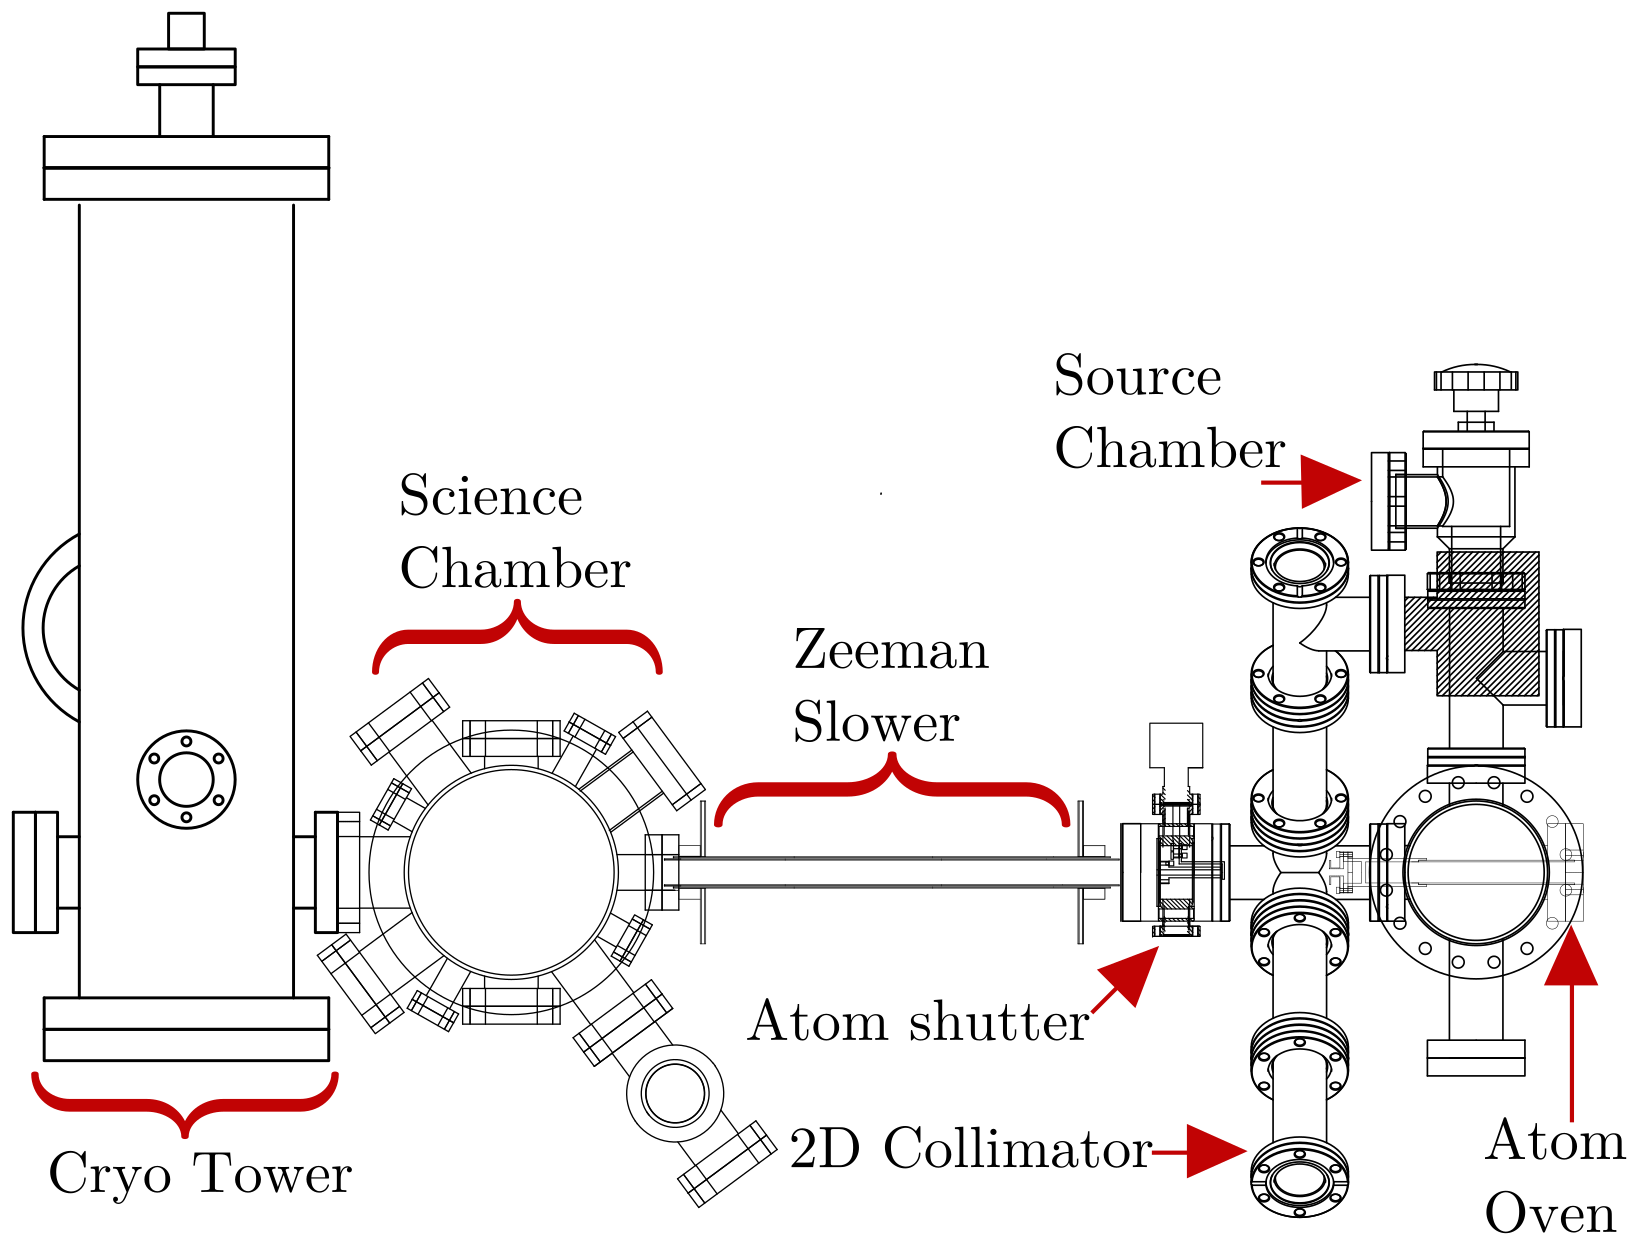
\includegraphics[width=\textwidth]{Vaccum_overview.png}}
		\caption{Neutral apparatus vacuum system}{Some components are rotated to provide easier identification. Not shown are the bellows which extend from the upper angle valve of the source chamber to the metal valve shown in Fig.\,\ref{fig:cryoTower}.}
		\label{fig:vacuumSystem}
	\end{figure}		
Figures \ref{fig:sourceSideView} - \ref{fig:cryoTower} also show various views of the atom source, 2D collimator, and cryo tower assemblies. Note the red markers and green arrows denote the positions of heater bands and thermo-couples respectively. For more information please see App. \ref{app:breakingVacuum}.
	\begin{figure} 
		\centerline{
		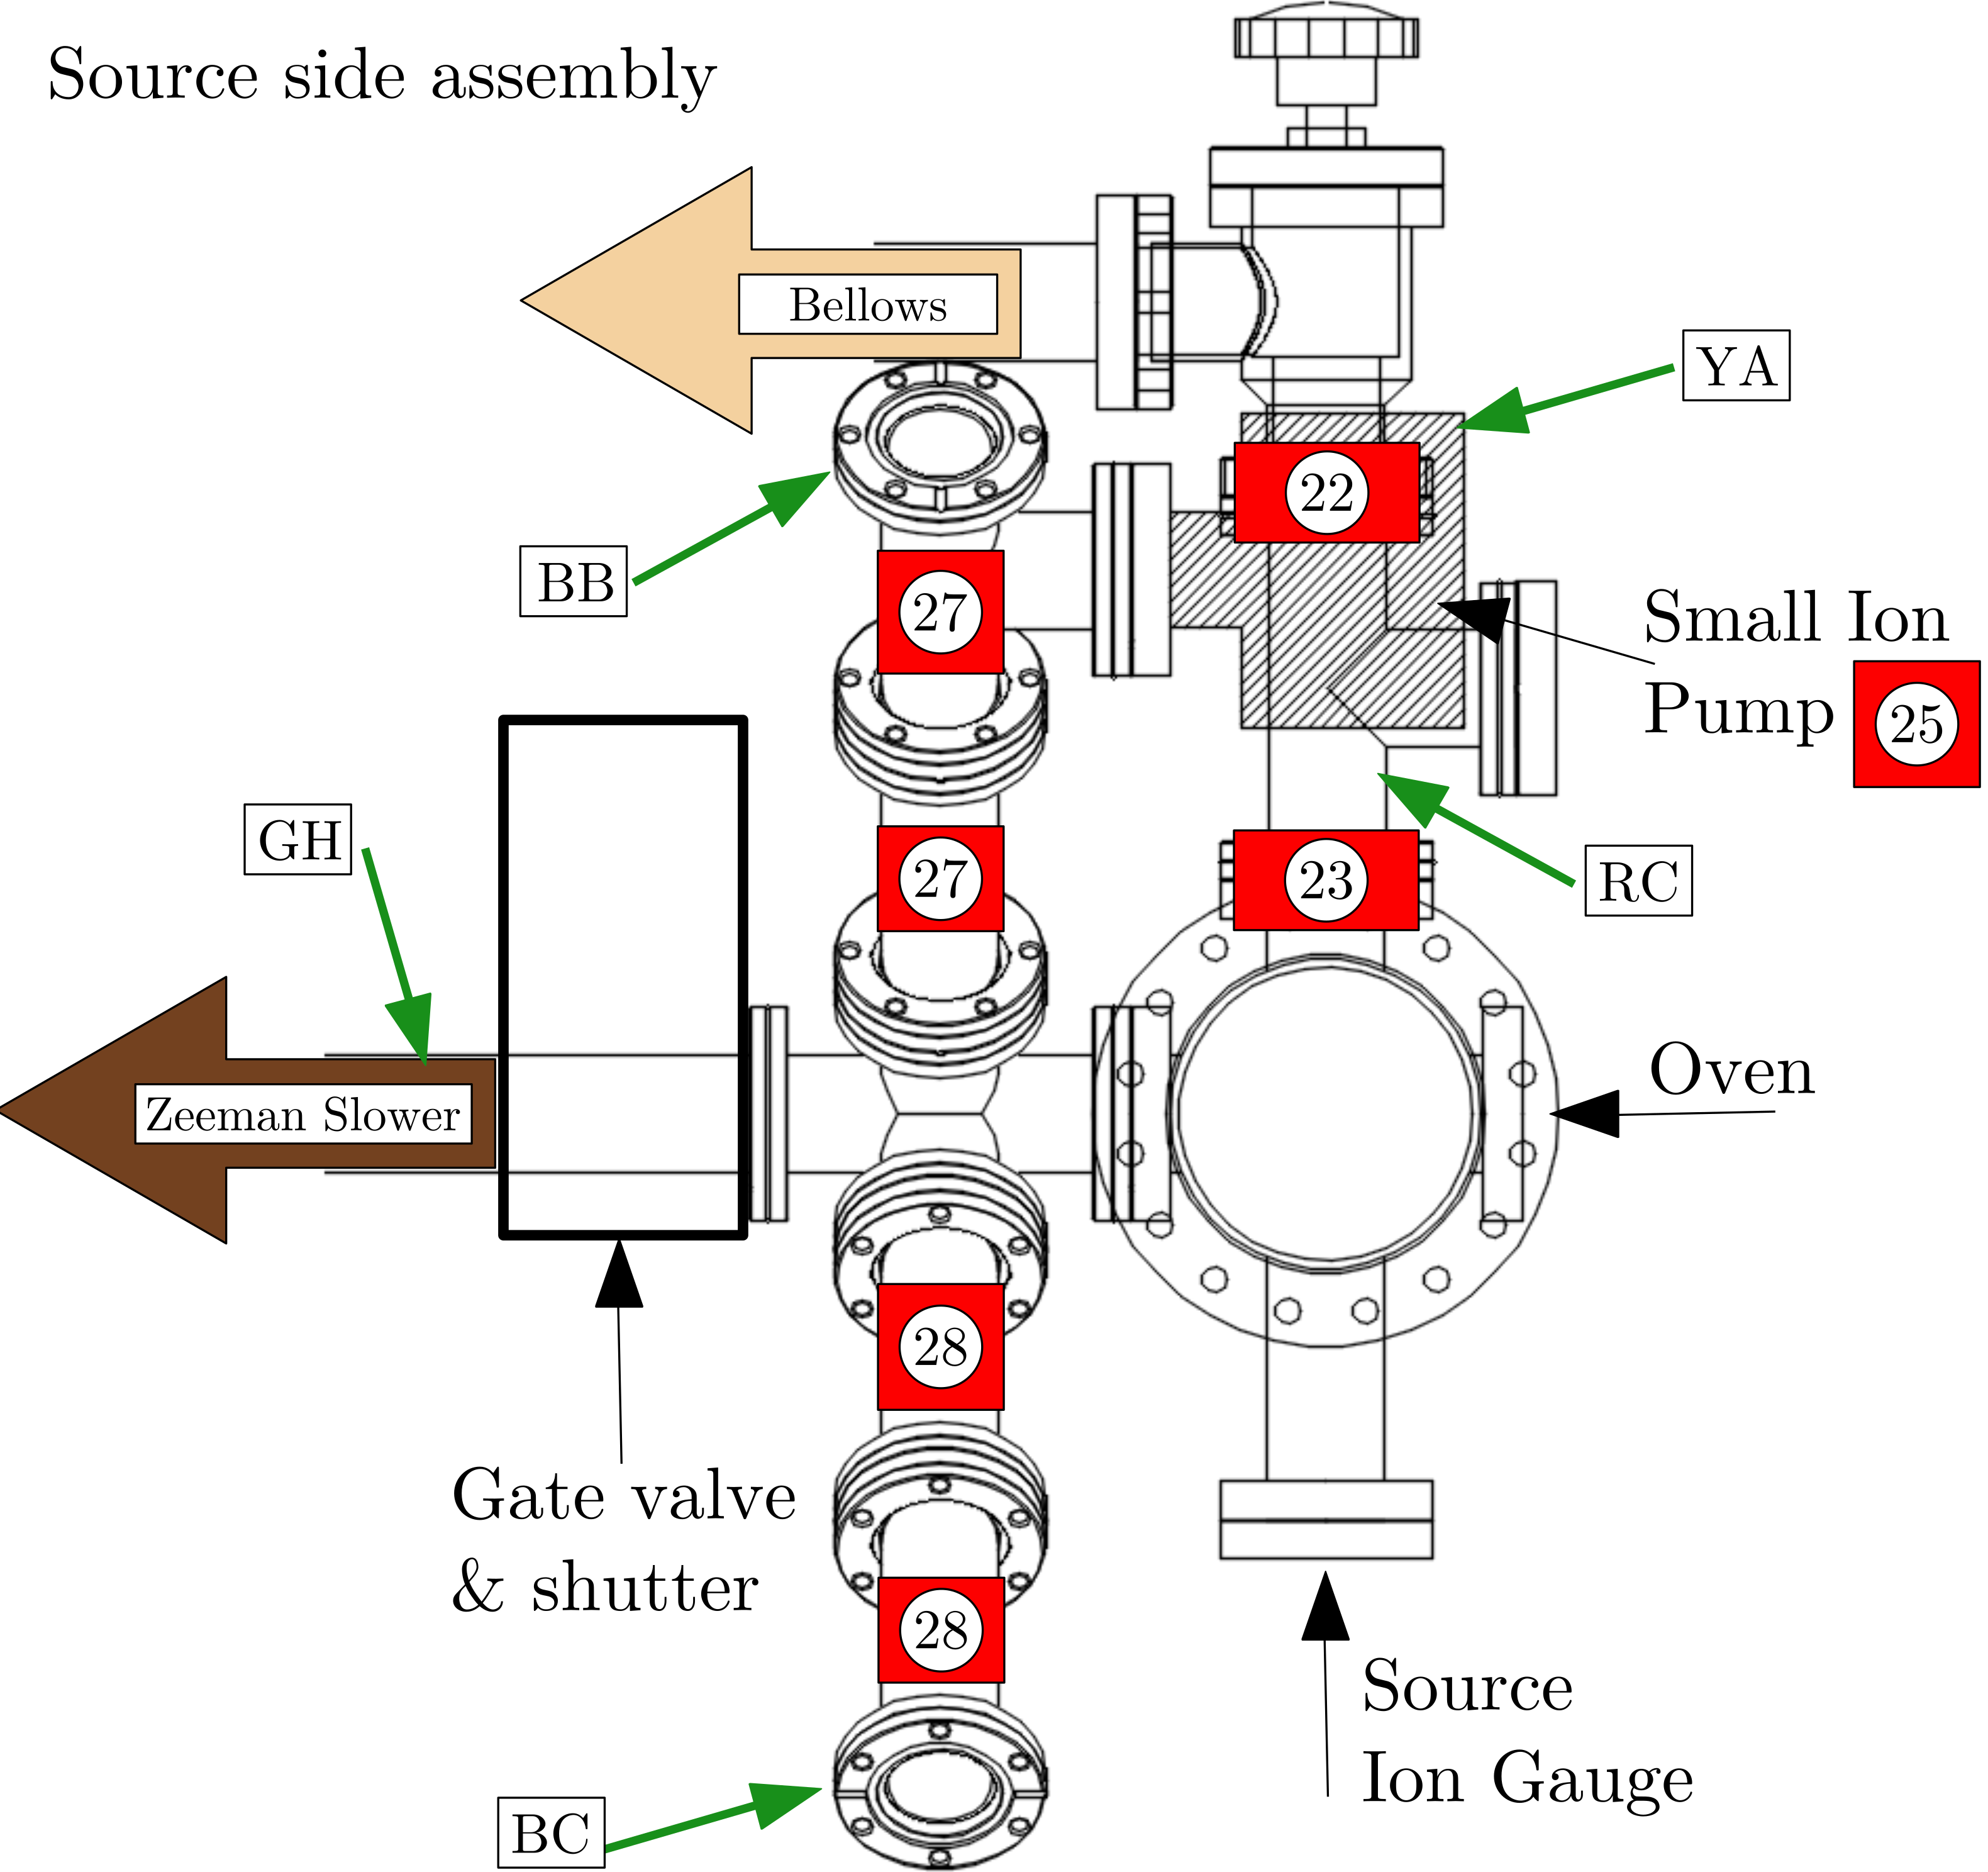
\includegraphics[height=0.4\textheight]{vacuum_source_assembly.png}}
		\caption{Source assembly - side view}
		\label{fig:sourceSideView}
	\end{figure}
	
	\begin{figure} 
		\centerline{
		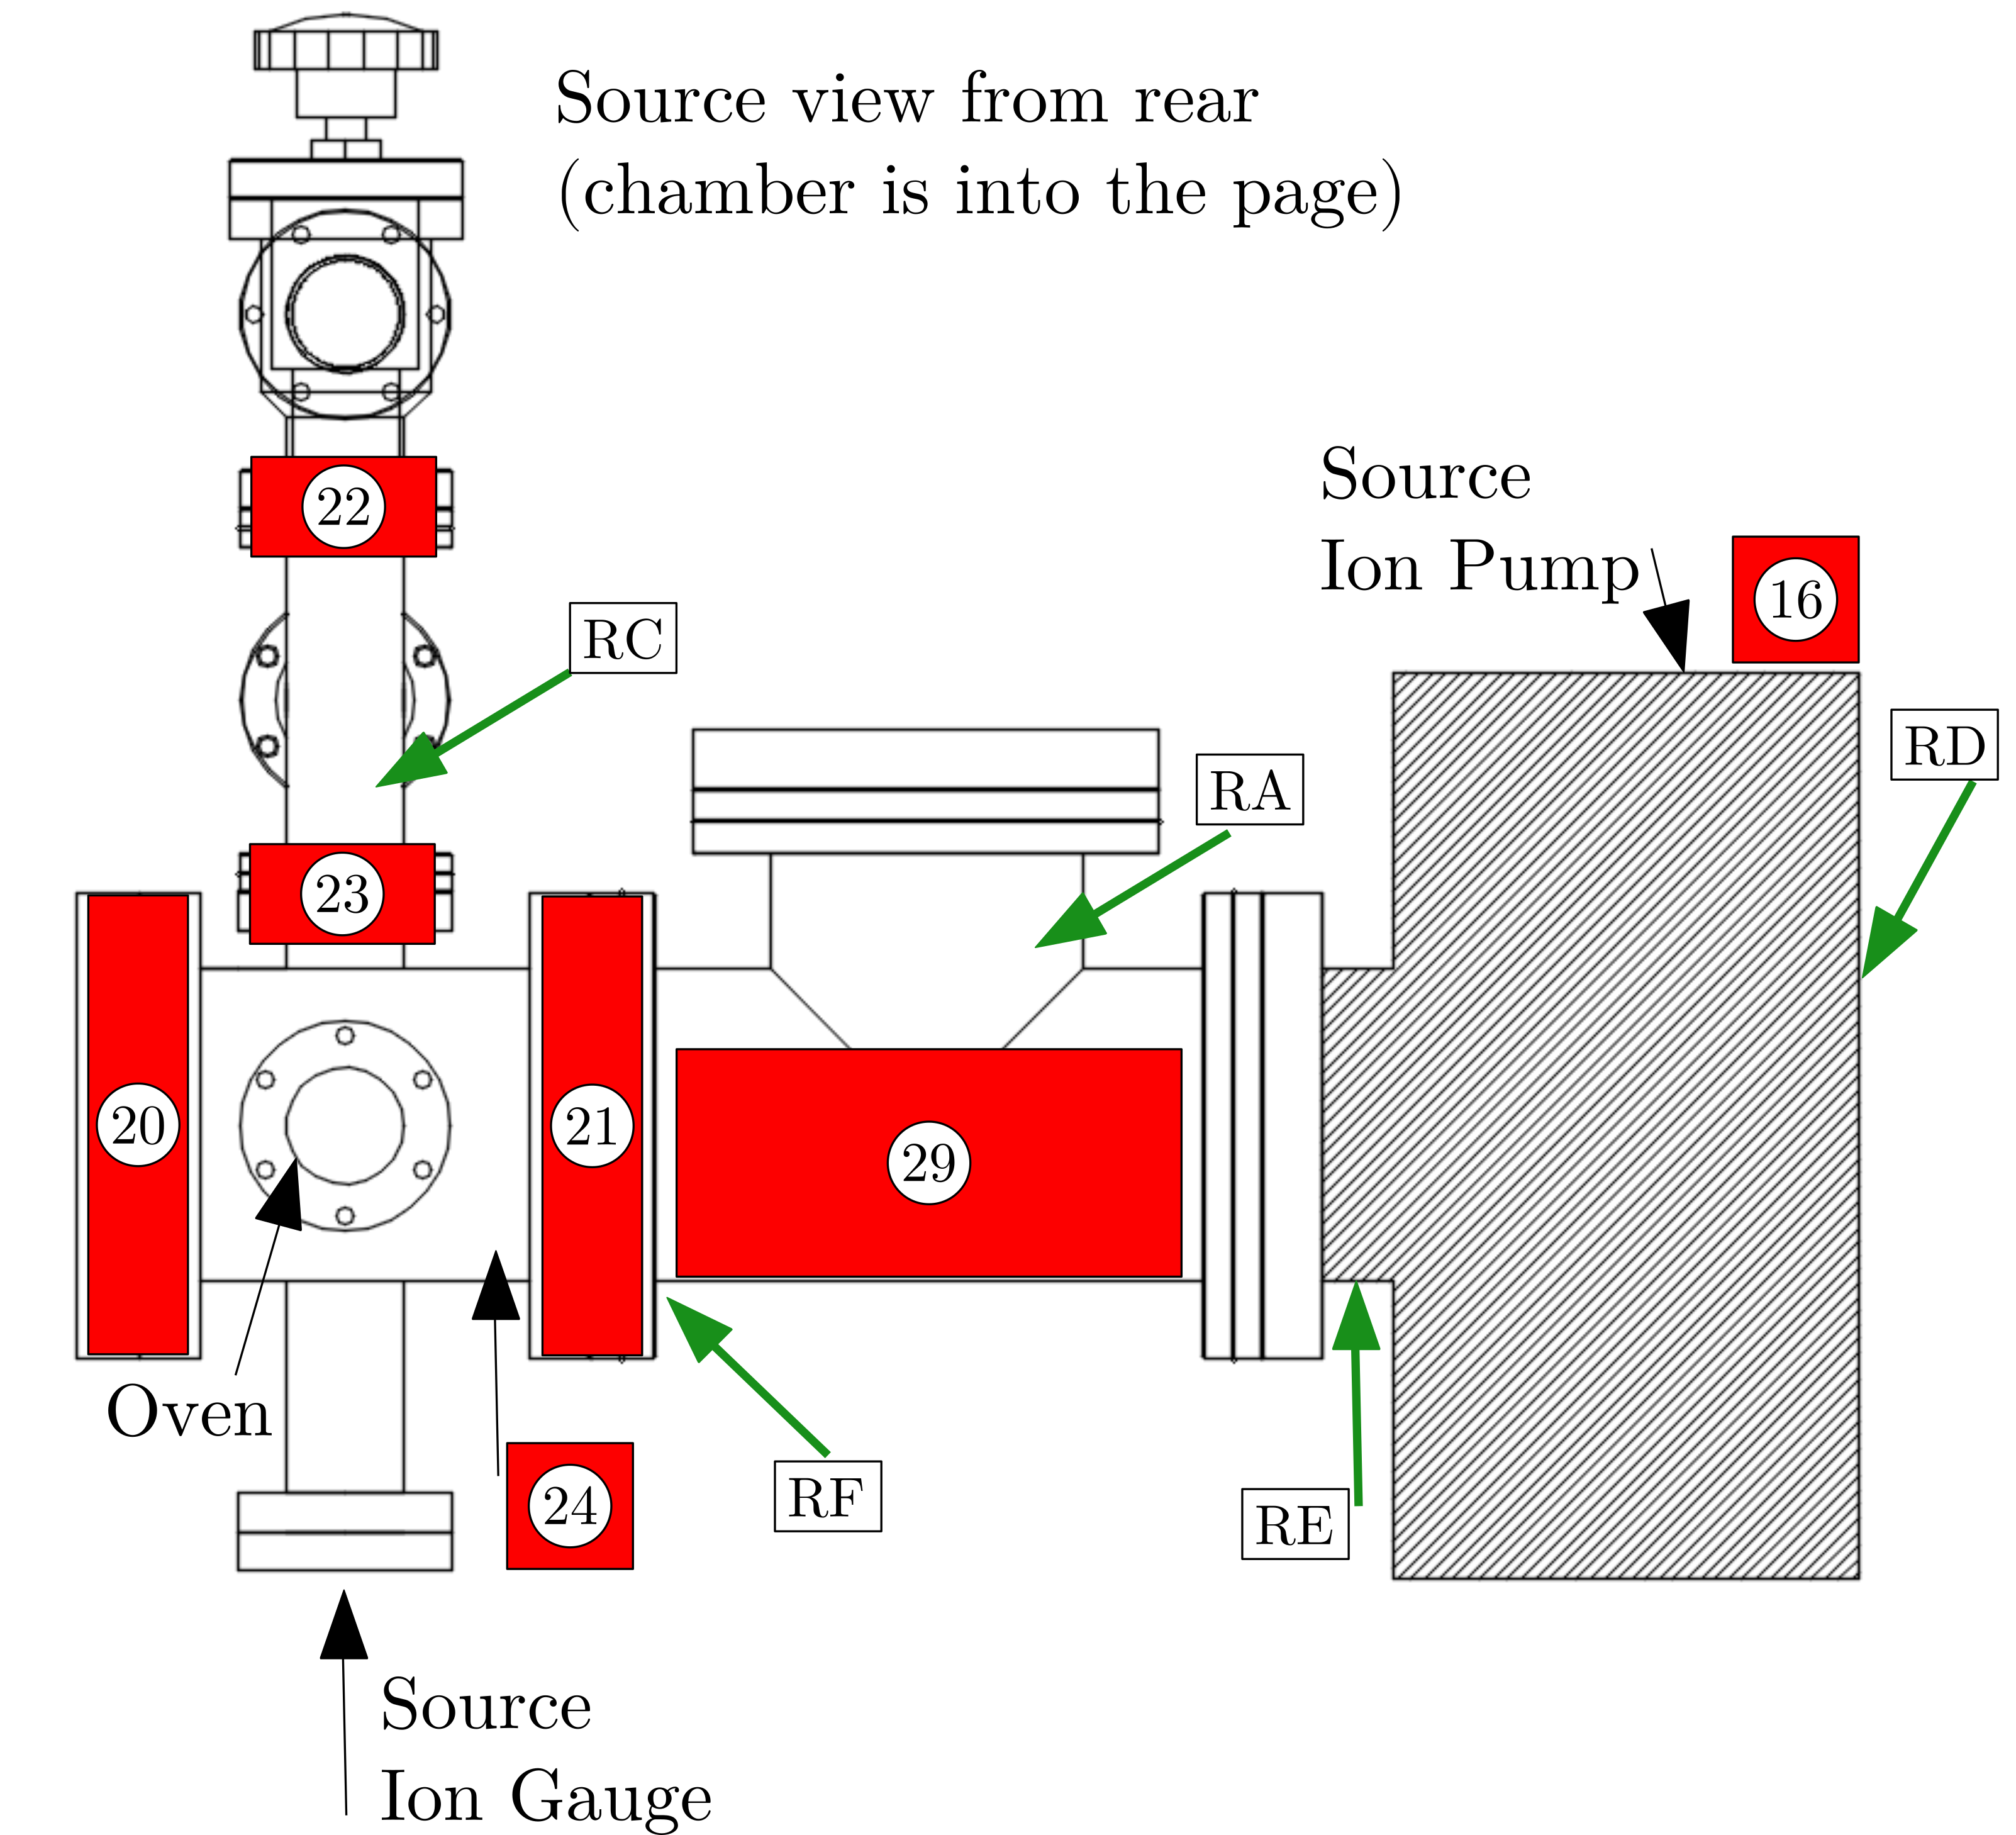
\includegraphics[height=0.4\textheight]{vacuum_source_rearView.png}}
		\caption{Source assembly - rear view}
		\label{fig:sourceRearView}
	\end{figure}
	
	\begin{figure} 
		\centerline{
		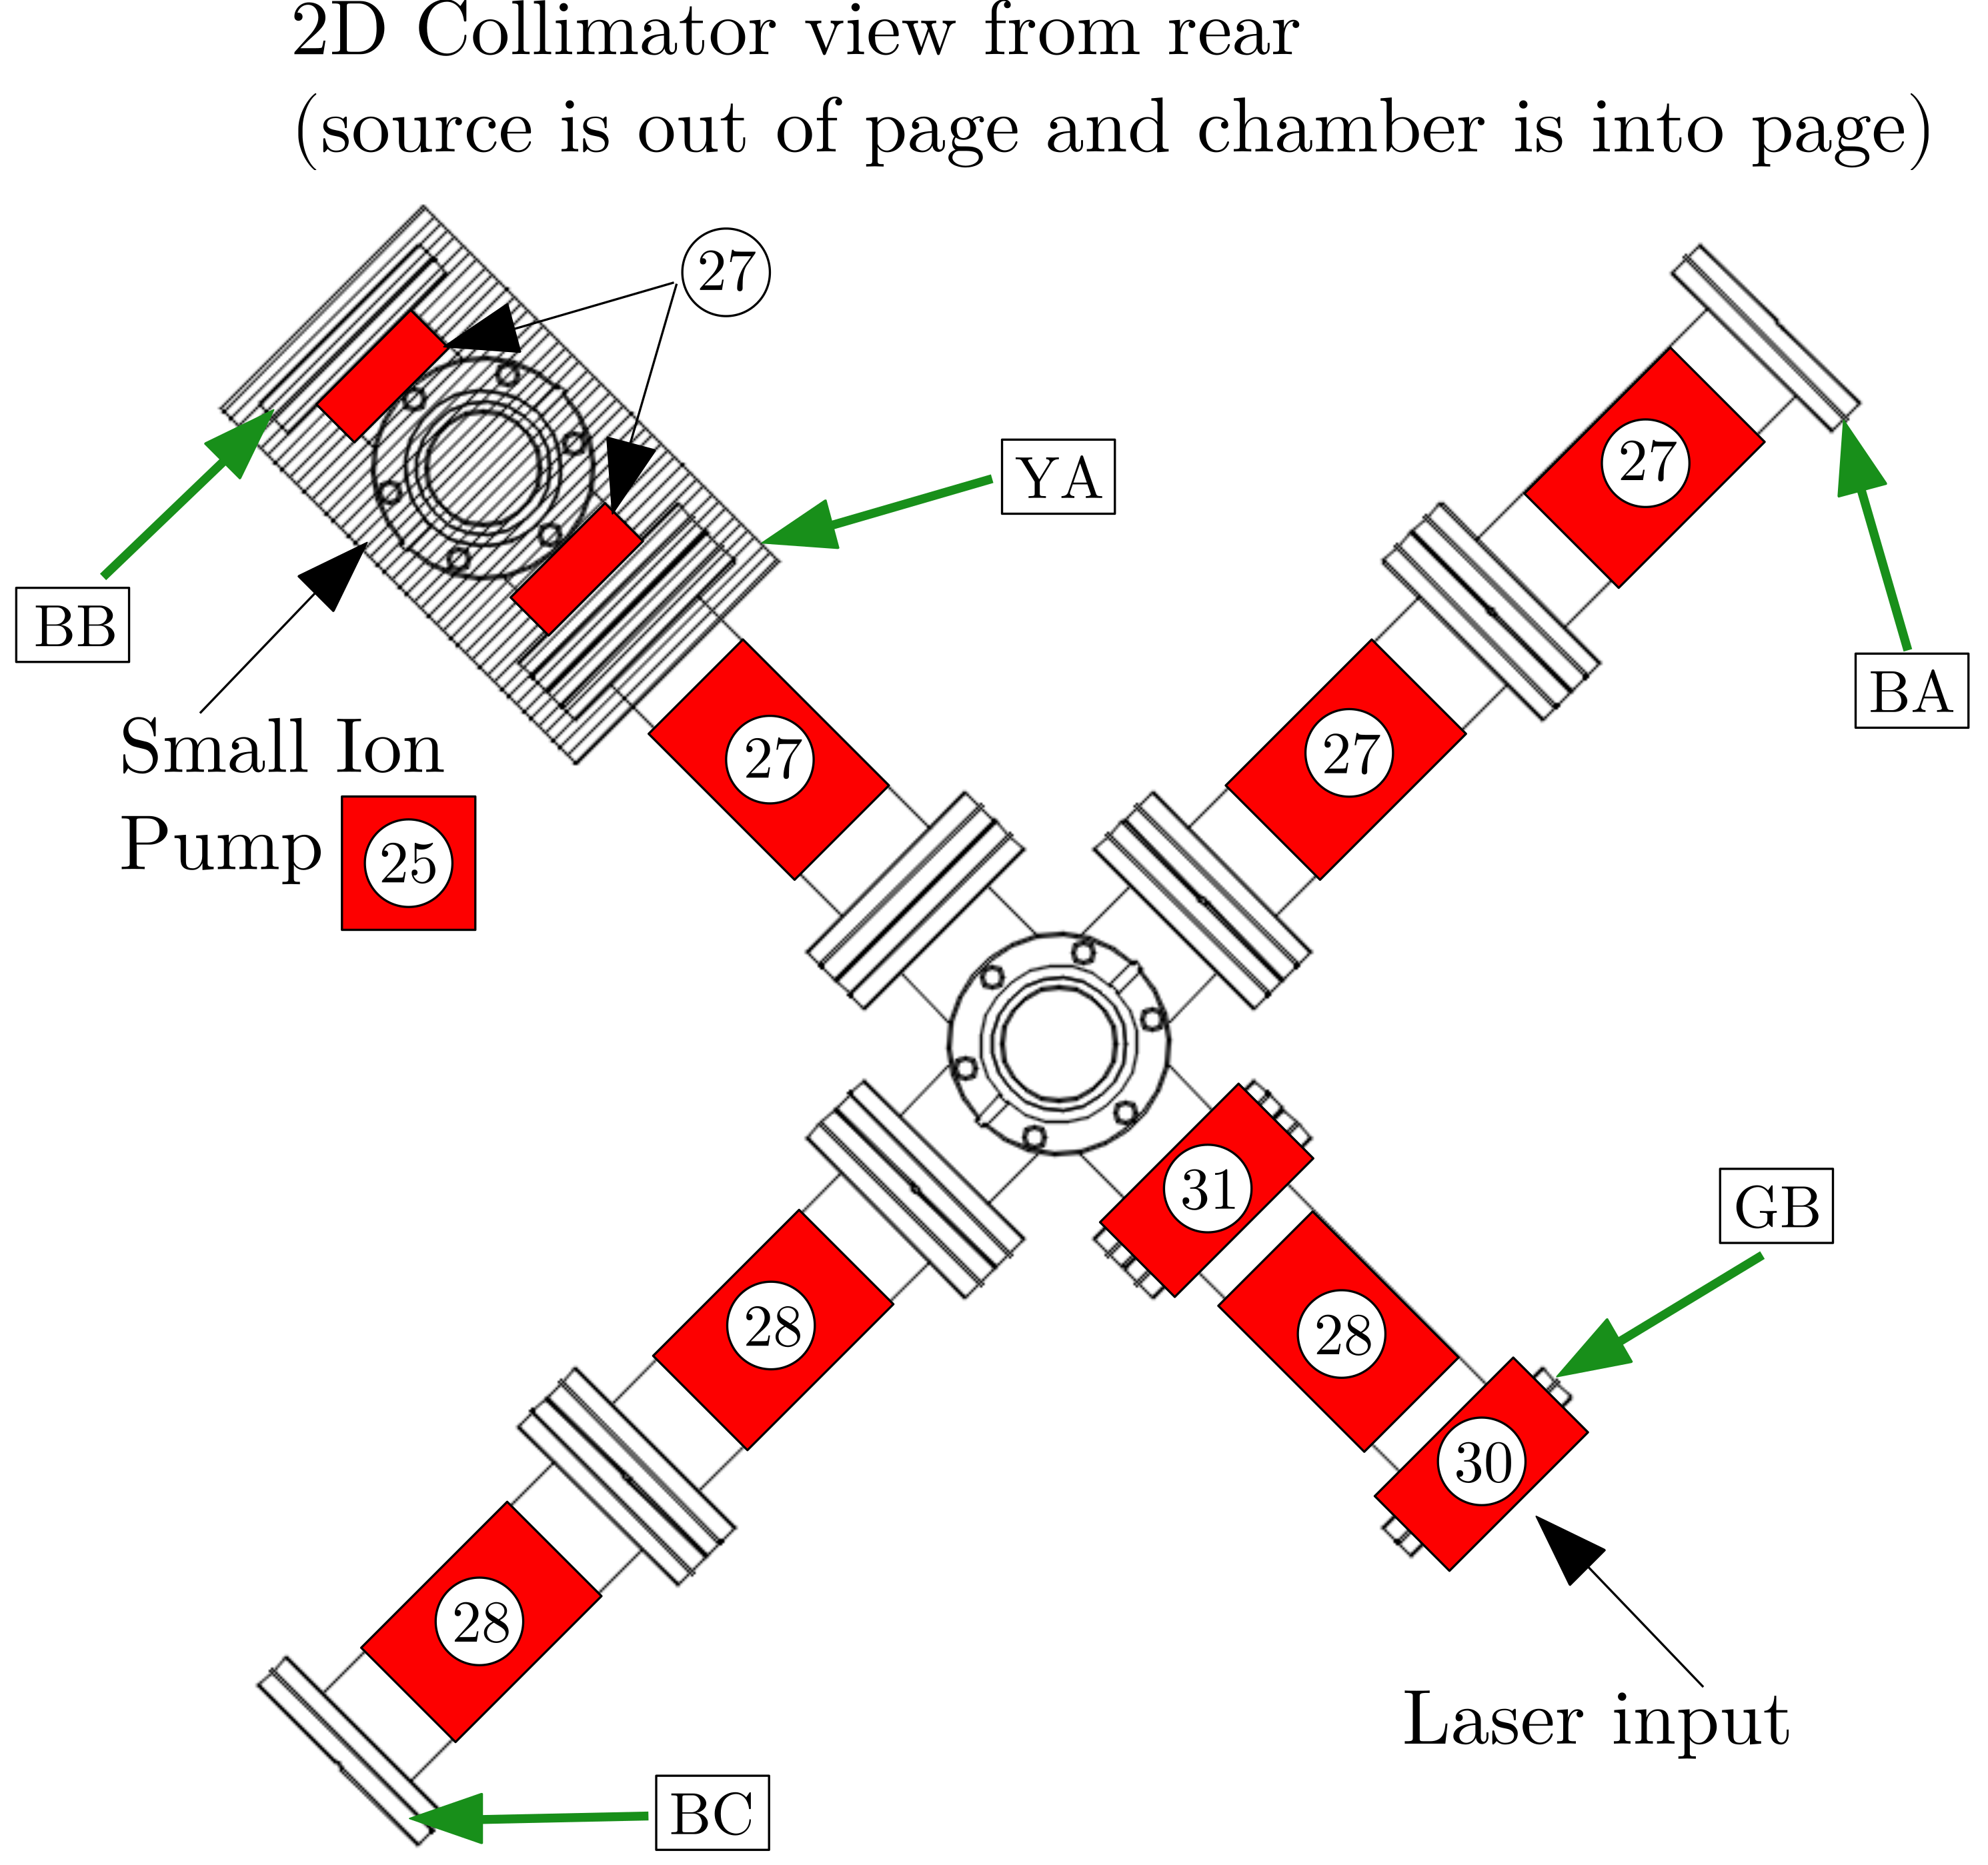
\includegraphics[height=0.5\textheight]{vacuum_2D_collimator.png}}
		\caption{2D collimator assembly}
		\label{fig:assembly_2Dcoll}
	\end{figure}
	
	\begin{figure} 
		\centerline{
		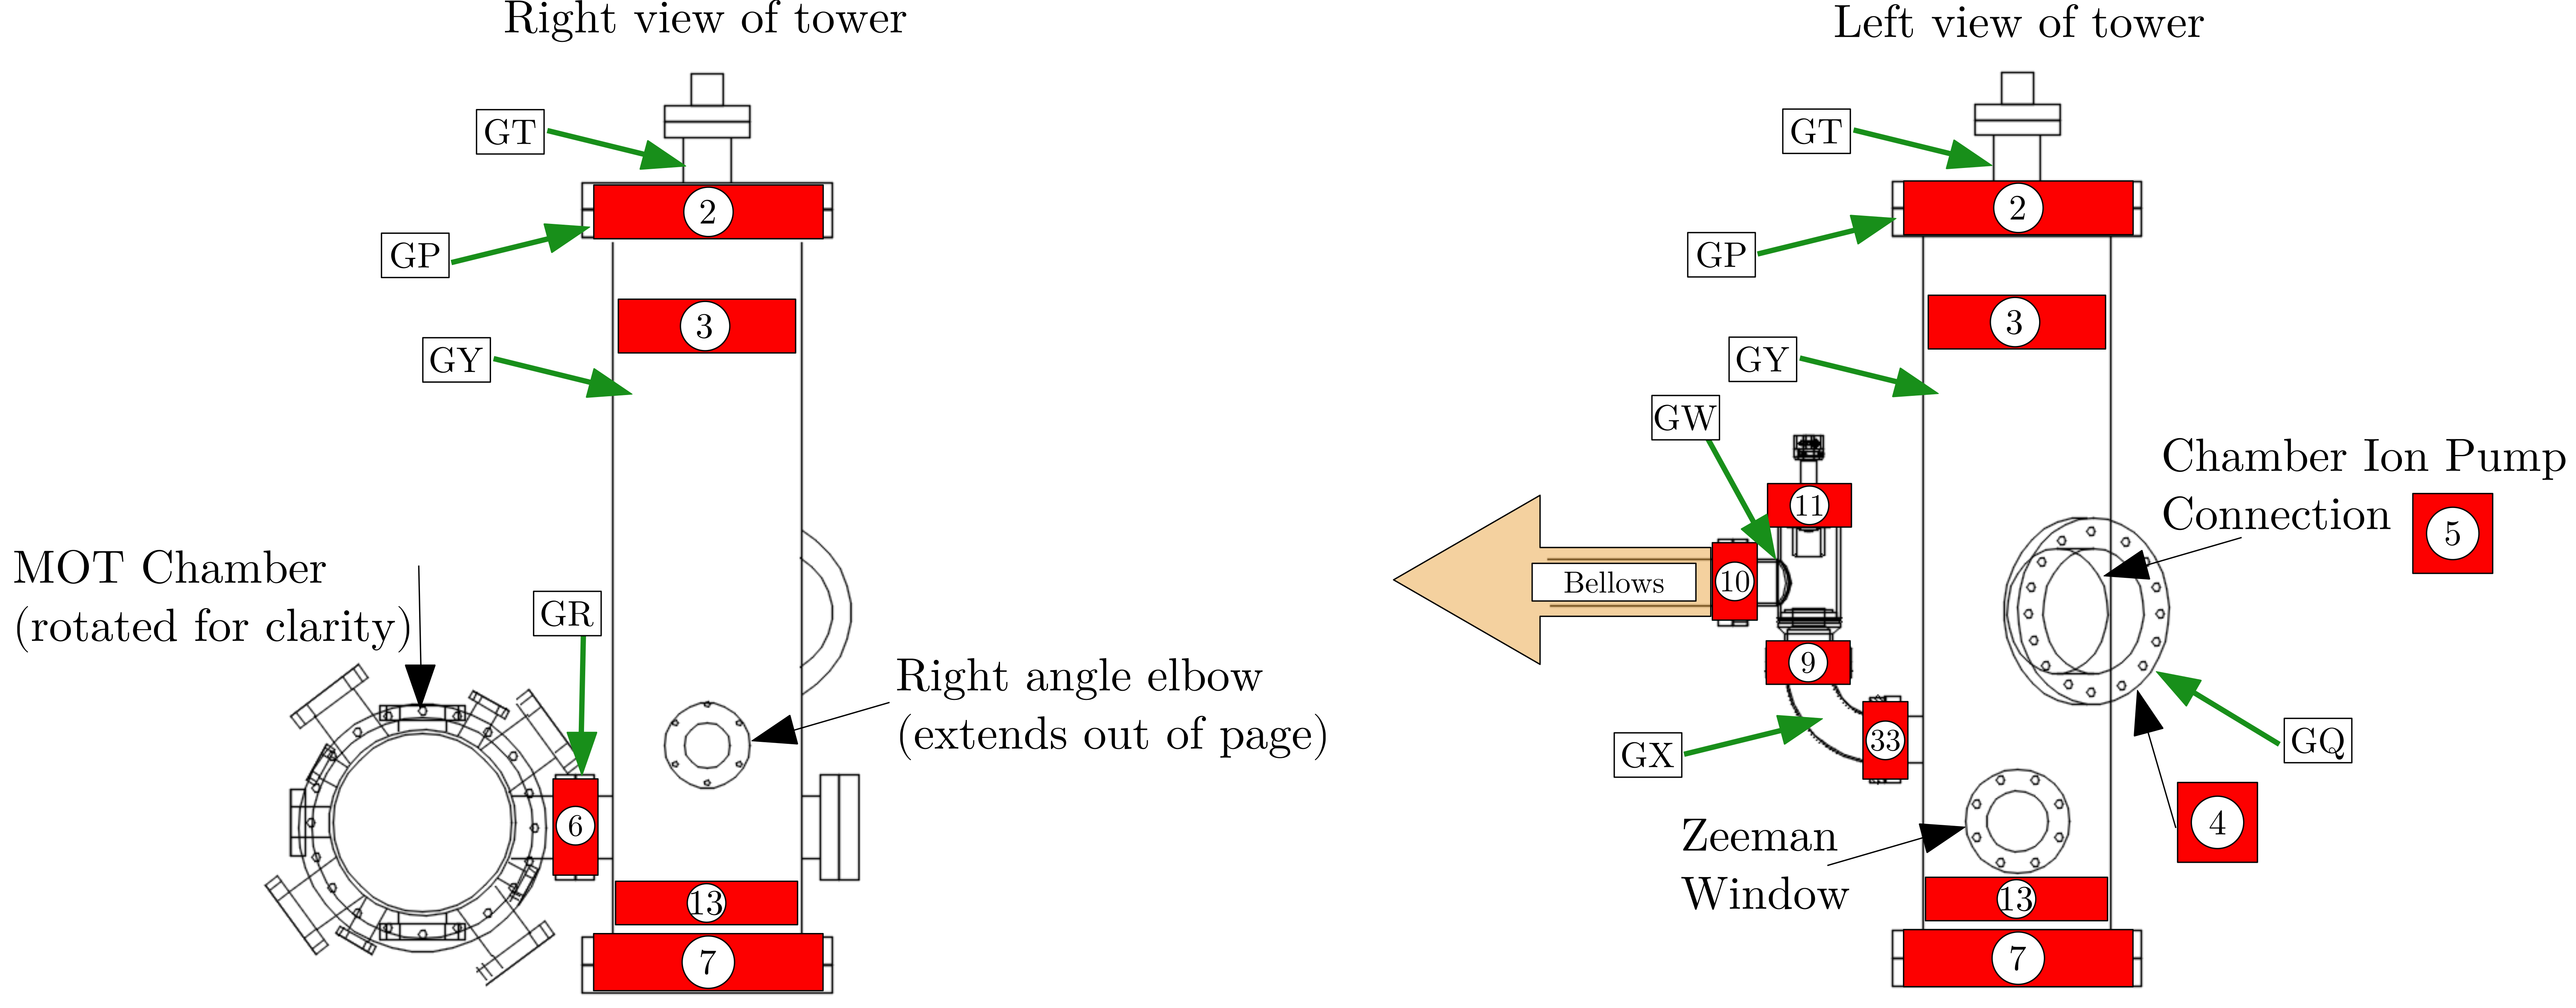
\includegraphics[width=1.25\textwidth]{vacuum_tower.png}}
		\caption{Cryo tower assembly}
		\label{fig:cryoTower}
	\end{figure}
From right to left, the system starts with an oven source based around a custom nozzle design which uses a rod heater to vaporize elemental strontium.
Next, there is a 6 way tee used for the optical molasses step which we refer to as the 2D collimator. 
From here atoms pass through a narrow differential pumping tube and into the entry port of the Zeeman slower where a majority of the laser cooling takes places as atoms traverse the 10.5\,inch one dimensional cooling stage. 
Following the Zeeman slower, atoms enter the science chamber where a plethora of lasers are used to manipulate and probe their behavior.
Chief among these laser systems are the MOT sequences and high intensity far off-resonant optical dipole traps used for the final stage of confinement.
Lastly, the body of the science chamber is supported by the cryo tower which houses a titanium sublimation catridge (model: Varian 916-0061 series) and is the entry point for the Zeeman laser.
It is worth explicitly noting that this Zeeman window is necessarily directly opposite the atomic source and therefore is subject to a flux of hot atomic strontium which will eventually coat the vacuum side. A brief note on a possible solution to this problem is explored at the end of this section.

While the source and science chamber have remained largely unchanged since the publication of Natali's thesis, several key improvements and events have occurred over the last few years\footnote{As of April 2019, the most up to date CAD drawing for the Neutral apparatus is located at \texttt{KillianDrobo:\textbackslash Neutral\textbackslash Laboratory Systems\textbackslash Vacuum Chamber\textbackslash Neutral Chamber\textbackslash 2017.12.26\_strontiumvacuum35\_latticetable.dwg}. Additionally, please consult the README file located in this folder for further information.}.
These differences will be the subject of our discussion in the latter part of this section.


% Orientation of lasers to chamber 
Fig \hl{something} shows a closer view of the science chamber and defines a coordinate system as well as directional labels used throughout this thesis. 
We will use this reference when illustrating the orientation of various lasers through the science chamber to help the reader.

The original drawings of these components can be found in App. A.10 of \cite{MartinezdeEscolar2010} along with detailed information on the window coatings.

\paragraph{Recent changes}
\subparagraph{Addition of platform:}
While exploring routes to produce quantum degenerate gases of strontium, it was determined that different geometries of traps were necessary to achieve efficient forced evaporation. 
The task of redesigning the optical dipole traps was undertaken by Ying Huang and is detailed in her master's thesis \cite{Huang2013}. 
As part of this project, a raised platform was designed and built around the chamber to facilitate beam shaping and launching of the ODT laser.
Details of the platform are available in the main apparatus CAD drawing.
%Unfortunately, while a major portion of this platform design is available in the main apparatus CAD file, the platform opposite of the oven is not documented.
%Nor is there a complete assembly drawing incorporating the chamber and platform, which may confound future efforts to build around the chamber as more complexity is introduced. 

The raised platform has become the primary method for directing lasers into the chamber including the 1064\,nm bulk optical dipole trap and the 532\,nm optical lattice, both of which are outlined below. 
During installation of the free space optical lattice we observed heating and hypothesized that relative movement of the platform and chamber may be a cause.
Supporting struts were then added beneath the chamber in an attempt to secure it to the platform around 2016.
However, the extreme sensitivity of cold atoms and occasional observation of shot to shot fluctuations persists the concern of relative movement between non-rigid components.

These concerns were reinforced when we observed increased stability with the addition of a partial cover over the platform optics for the optical dipole and lattice traps. 
Initially meant as an optical safety measure for enclosing the high power beams, the cover led to a marked decrease in shot to shot fluctuations of the cloud position after a time of flight.
With further testing we were able to attribute the increased stability to a mitigation of air currents caused by close proximity of the platform optics to the ventilation system meant to thwart dust accumulation inside the experimental enclosure.

% Running out of strontium
\subparagraph{Running out of strontium:}
In the winter of 2017 the neutral apparatus had been under vacuum for approx 8 years when suddenly we were no longer able to trap a significant number of atoms \footnote{It is was expected any trapping loss due to low strontium would be gradual and we were not able to determine the cause of the abrupt behavior.}.
After extensive testing, we hypothesized that we had run out of elemental strontium within the atomic source.
This led us to break vacuum, reload strontium, and perform a light bakeout procedure to reestablish the requisite ultrahigh vacuum for experiments.
Details of this bakeout procedure can be found in App. \ref{app:breakingVacuum}. 
Through this process we confirmed our hypothesis that lack of strontium was the cause of the issue. 
Figure \ref{fig:2d_coll_flourescence} shows the atom beam fluorescence after refilling the oven.
This image was taken while using the Zeeman laser to cause photon scattering and looking down the 2D collimator.
	\begin{figure}
		\centerline{
		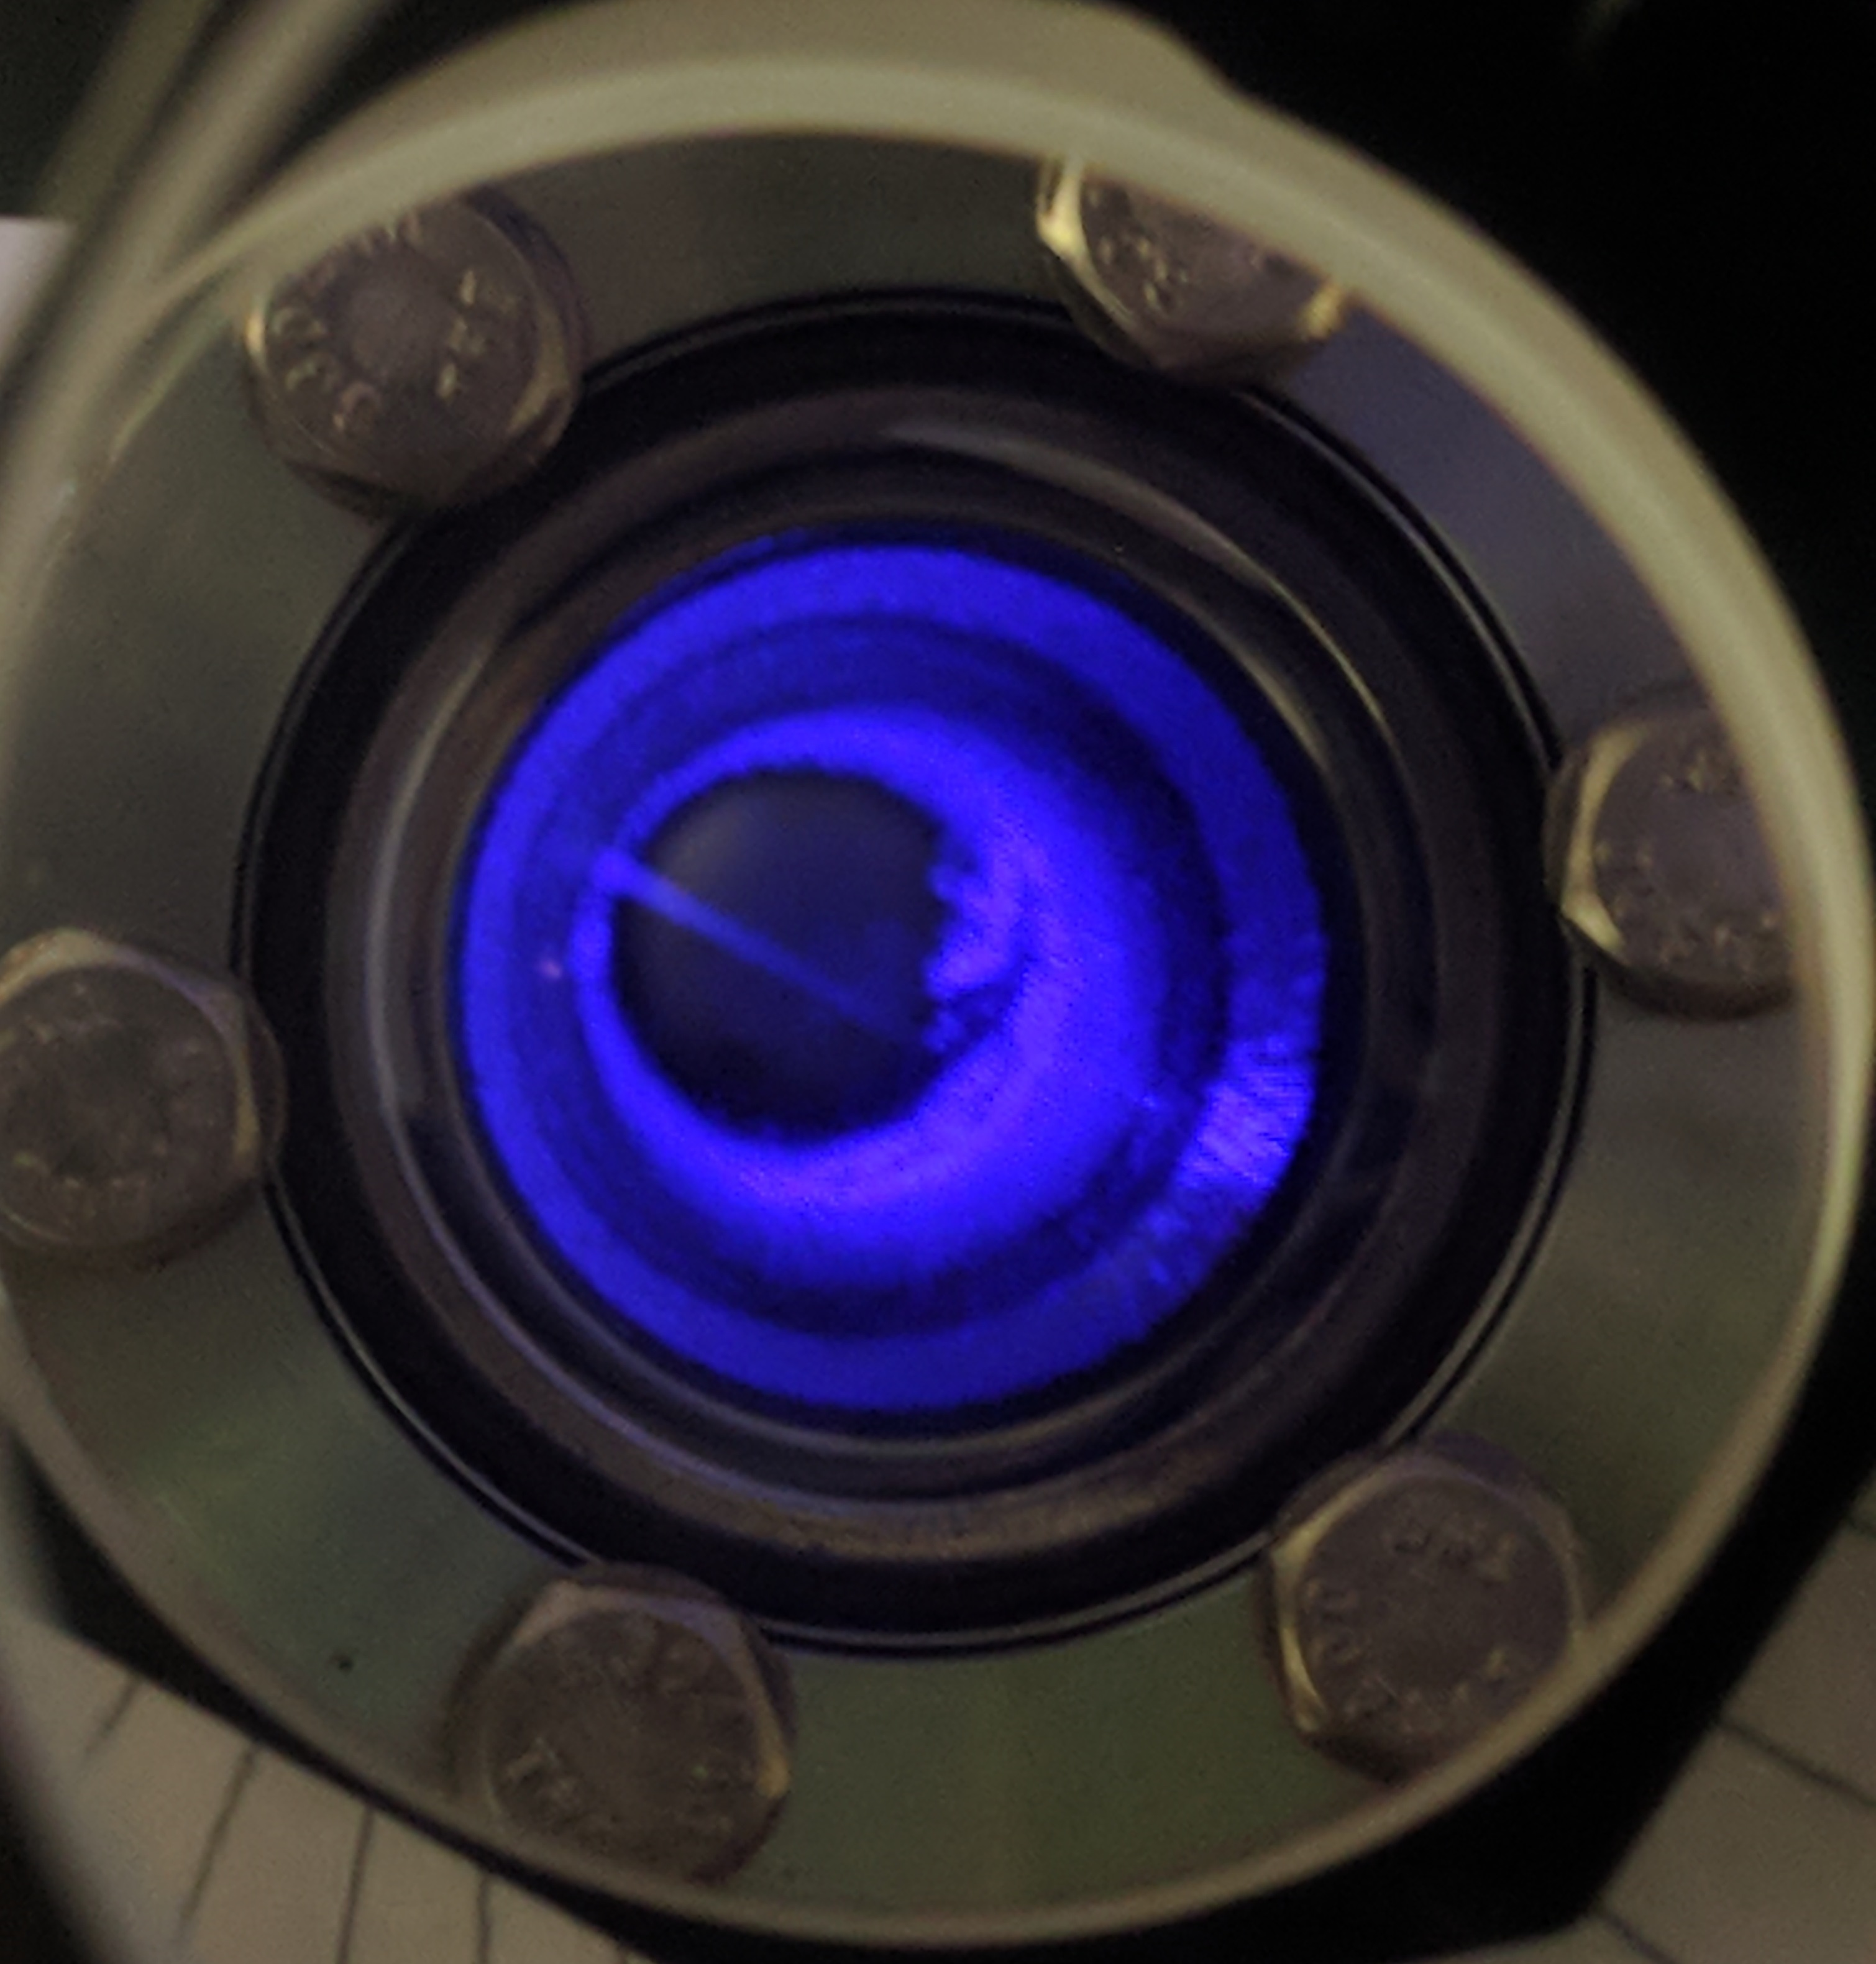
\includegraphics[height=0.5\textheight]{vacuum_IMG_20171103_184vacuum_230.jpg}}
		\caption{Typical fluorescence of Zeeman beam looking down 2D collimator}{This view is found using a 2 in mirror aligned along the path of the first pass of the 2D collimator and looking down the collimator tube. While looking at this angle, we are able to see the Zeeman beam move across the atom column when moving the last turning mirror. Reduction in this fluorescence signal from that shown was the primary indicator of lack of strontium in the source.}
		\label{fig:2d_coll_flourescence}
	\end{figure}  
Prior to this event the Neutral apparatus enjoyed lifetimes of approx. 25s as measured by background lifetimes measurements within the IR optical dipole trap. 
Approximately a year after restoring vacuum we have measured lifetimes on the order of 15s, the cause of the discrepancy is not rigorously known.

During the process of breaking vacuum we attempted several upgrades to the apparatus including adding a gate valve between the cryo tower and the Zeeman window and redesigning the atom nozzle source to incorporate a fixed heat shield around the heating element. 
Details of the nozzle design can also be found in App. \ref{app:breakingVacuum}.
Unfortunately, multiple issues arose during construction which led us to re-establish vacuum without these upgrades in place.
Therefore, they are documented in the appendices for potential future use.

Finally, after removing the atom oven to replace strontium, we placed a temporary viewport to facilitate alignment of the Zeeman beam through the length of the vacuum system. 
While aligning we observed an unexpected partial occlusion of the Zeeman beam and upon further investigation learned that the differential pumping tube is noticeably not parallel to the atom trajectory.
We were not able to determine the severity of the misalignment since the tube is not easily accessible and replacement is problematic as the tube is attached to a copper gasket held between flanges connecting the atom source chamber and the 6-way tee of the 2D collimator. 
The main readily measurable symptom is the occlusion of the Zeeman beam, which with an input power of approx. 120 mW before expansion optics and entering the chamber, only measures approx. 60 mW of transmitted power through the length of the vacuum system. 
A solution to bend the soft copper with a rod was proposed but abandoned due to concerns of cracking the thin copper.
As adequate repair of the tube necessitates a drastic and practically infeasible deconstruction of the vacuum system our goal here is to document the issue for future students.
It is currently hypothesized that this problem is the primary cause of the much longer load times needed in the Neutral apparatus compared to the newly designed Rydberg machine.

\paragraph{Clarifications from de Escobar thesis}
\subparagraph{HV version 1 \& 2:}
As a point of clarification, Natali's thesis \cite{MartinezdeEscolar2010} presents two versions of the HV chamber in figures A.42 - A.47 while referencing that the original construction proceeded with version 1. 
However, version 2 (the cryo tower) was installed around 2011 and is currently in use. Version 2 is shown in Fig.\,\ref{fig:cryoTower} and details are available in the apparatus CAD drawing.

\subparagraph{Collimating array in nozzle:}
% hypodermic needle nozzle
Once more, Natali's thesis refers to the installation of an improved nozzle design incorporating an array of collimating tubes constructed from 2$\mu$ hypodermic needles (model: \hl{find}). 
Modeling and construction of this design was done by Anton Mazurenko, \cite{Mazurenko2010}, with the goal of improving the angular discrimination of the oven assembly to produce a more highly collimated beam of atoms.
Figure \ref{fig:2010_nozzle} shows the improved nozzle design \footnote{For reference, this nozzle design is labeled "new nozzle summer 2010" in the apparatus CAD file to distinguish it from the other nozzle drawings also present.}.
	\begin{figure}
		\centerline{
		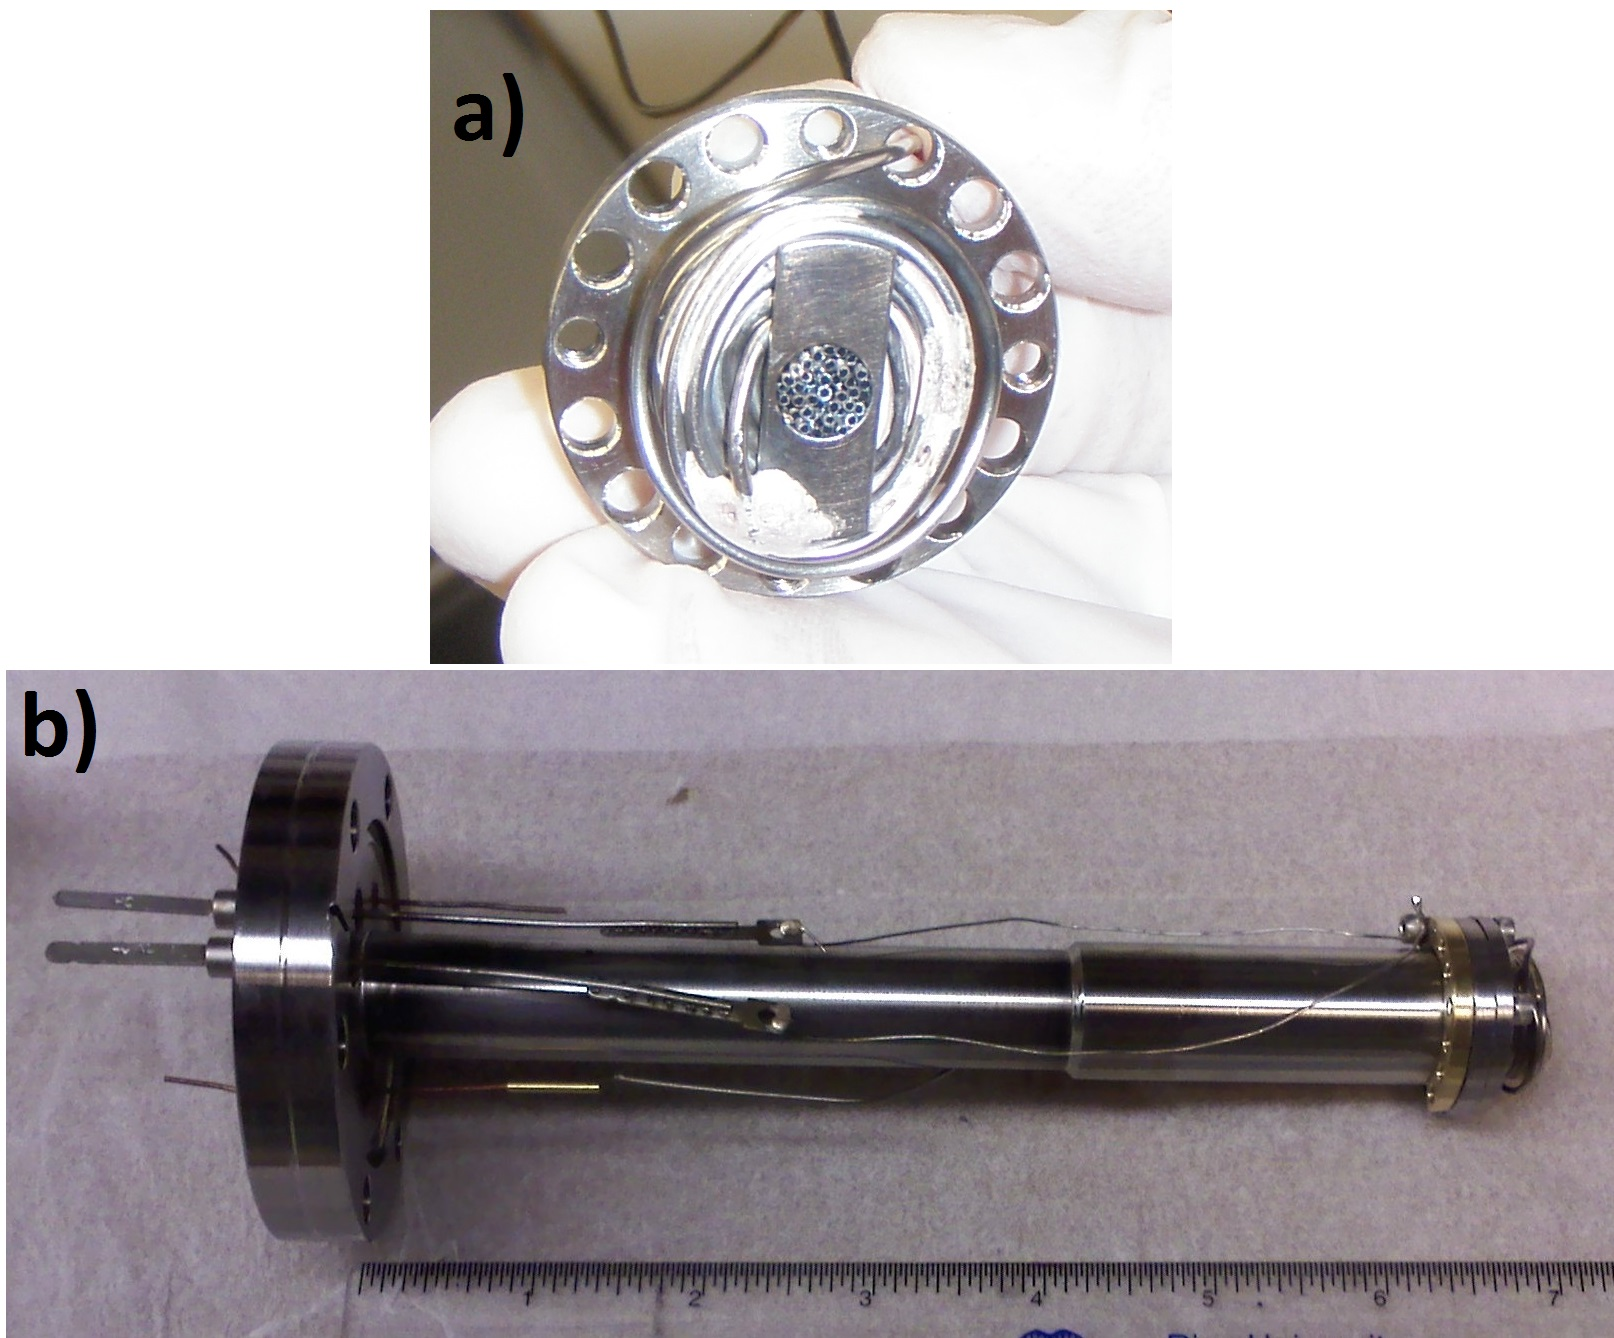
\includegraphics[height=0.4\textheight]{vacuum_nozzle.jpg}}
		\caption{Atom oven and nozzle construction}{a) The nozzle through which vaporized strontium enters the experiment. Here we see the array of collimating tubes behind which solid strontium is packed. b) The complete oven construction which houses the cartridge heater and the nozzle at the tip.}
		\label{fig:2010_nozzle}
	\end{figure}
The original assembly of this oven also incorporated a heat shield that would insert over the construction shown in Fig.\,\ref{fig:2010_nozzle}b) but this shield is not currently installed on the source oven.
%was ultimately abandoned since there was no way to fasten it to the flange which led the shield to fall off. 
 
\paragraph{Ablating strontium off window} \label{p:ablatingSr}
While not directly related to any experiment or typical procedure, this sub-section summarizes a brief side project of using a pulsed 532\,nm Verdi to ablate strontium from a vacuum window.
As discussed previously, a common problem faced by strontium experiments is the accumulation of strontium on the Zeeman entry port. 
These deposits may then act as a partial mirror leading to attentuation of the crucially important Zeeman beam. 
It was shared through private communication with professor Killian that pulsed 532\,nm light (such as from a q-locked Verdi system used in the Plasma laboratory) might vaporize the strontium off the window and restore any loss in transmitted Zeeman power. 
Using a test apparatus we were able to verify that indeed we could ablate the strontium off of an uncoated window, as shown in figure \ref{fig:ablating_strontium}.
	\begin{figure}
		\centerline{
		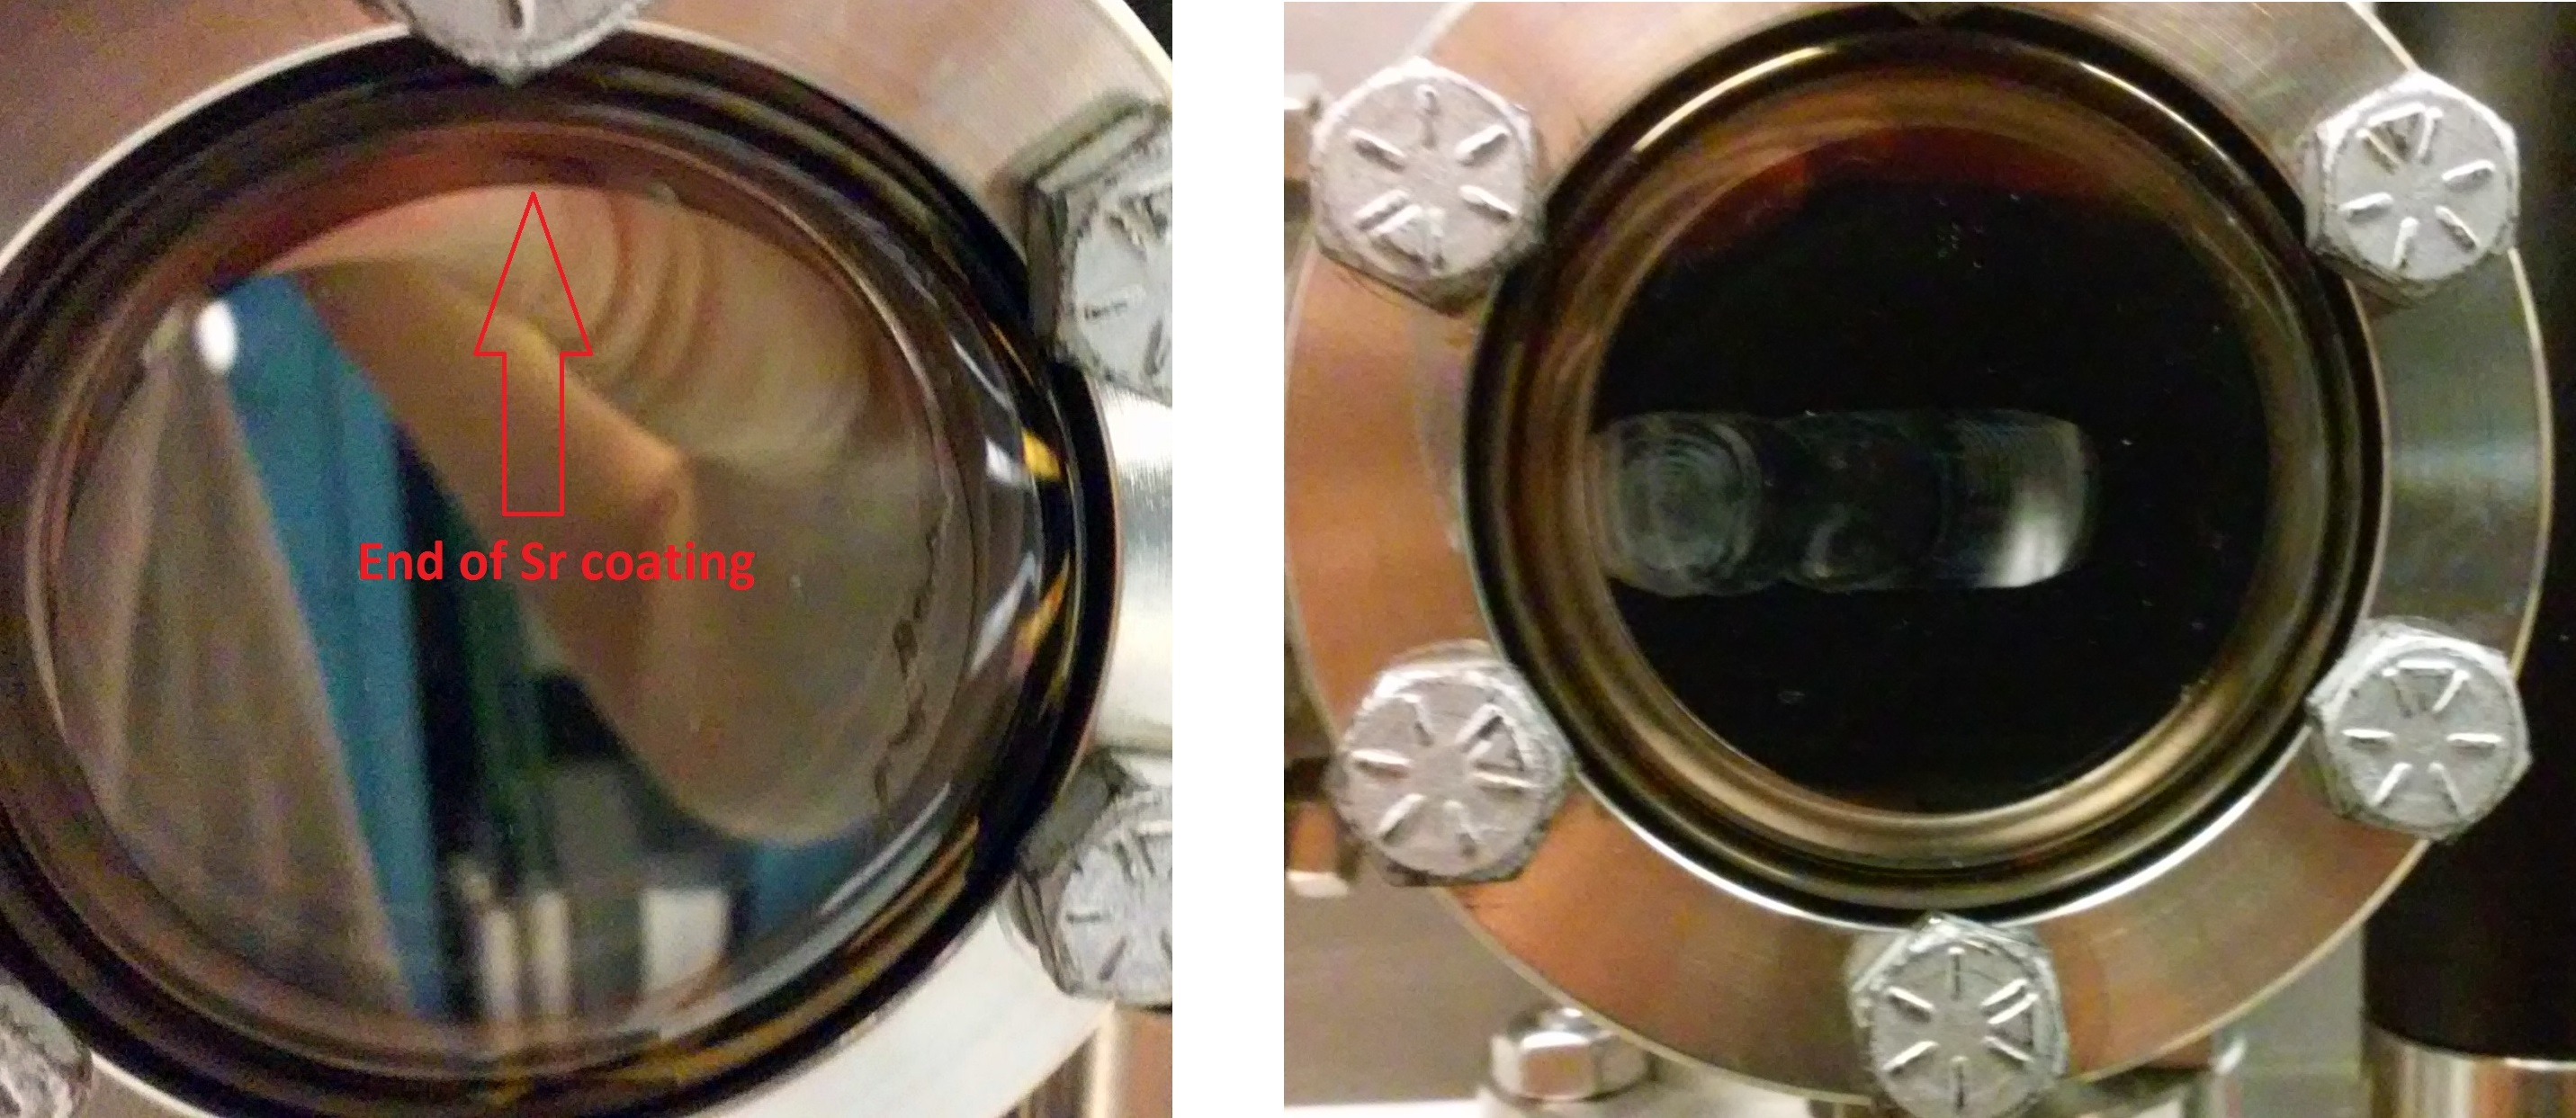
\includegraphics[width=0.8\textwidth]{vacuum_ablated_sr2.jpg}}
		\caption{Ablating strontium coating from window}{Comparison of the before (left) and after (right) when using a pulsed 532\,nm Verdi to ablate strontium. The residue visible in the after image we hypothesize to be caused by high pulse energy. We reduced the pulse energy as we moved towards the center of the window.}
		\label{fig:ablating_strontium}
	\end{figure}
This promising test led us to install an optical traversal port connecting the Plasma and Neutral labs. 
Unfortunately, while flashing the Verdi on a small section of the Neutral Zeeman window we found that the energy needed to ablate the strontium was accompanied by deformation of the window.
We discontinued the ablation upon observing this behavior to avoid further damage and we subsequently replaced the window after breaking vacuum as previously noted.

In an effort to mitigate the time the window is exposed to the hot strontium beam, we have also installed a small servo motor to drive the atom shutter valve and integrated this mechanism into the experimental runtime. 
This integration only opens the shutter during times of actively trapping atoms. 
Details of the servo motor trigger integration into the neuKLEIN control system are available in App \hl{somewhere}.

\pagebreak
\section{Laser systems}\label{sec:laser_systems}
\setcounter{footnote}{0}
The heart of any atomic physics experiment are the laser systems which are the basis for laser cooling and various probes.
Our lab has transitioned to mainly using diode lasers and relies heavily upon the use of injection locked master - slave setups. \hl{ref}
Below we will outline the specifics of our light generation systems.
In particular, future experiments on the Neutral apparatus aim to explore quantum magnetism using strontium 87 and as such we will emphasize several key changes which have been made to the 461 locking and 689 trapping systems to facilitate these experiments.

\subsection{Wideband cooling stage: 461\,nm} \label{ssec:461sys}
\subsubsection{Overview}
As discussed in the experimental overview, the majority of our laser cooling is done using 461\,nm light. 
We generate and control these photons by amplifying and frequency doubling 922\,nm light from a master ECDL diode laser. 
Fig.\,\ref{fig:461blockSys} shows an overview of how we generate and use the 461\,nm light.
We will explore each of these sections in detail below, with emphasis on the MOT sub-system since it is the basis for many different components of the overall 461 generation.
	\begin{figure}
		\centerline{
		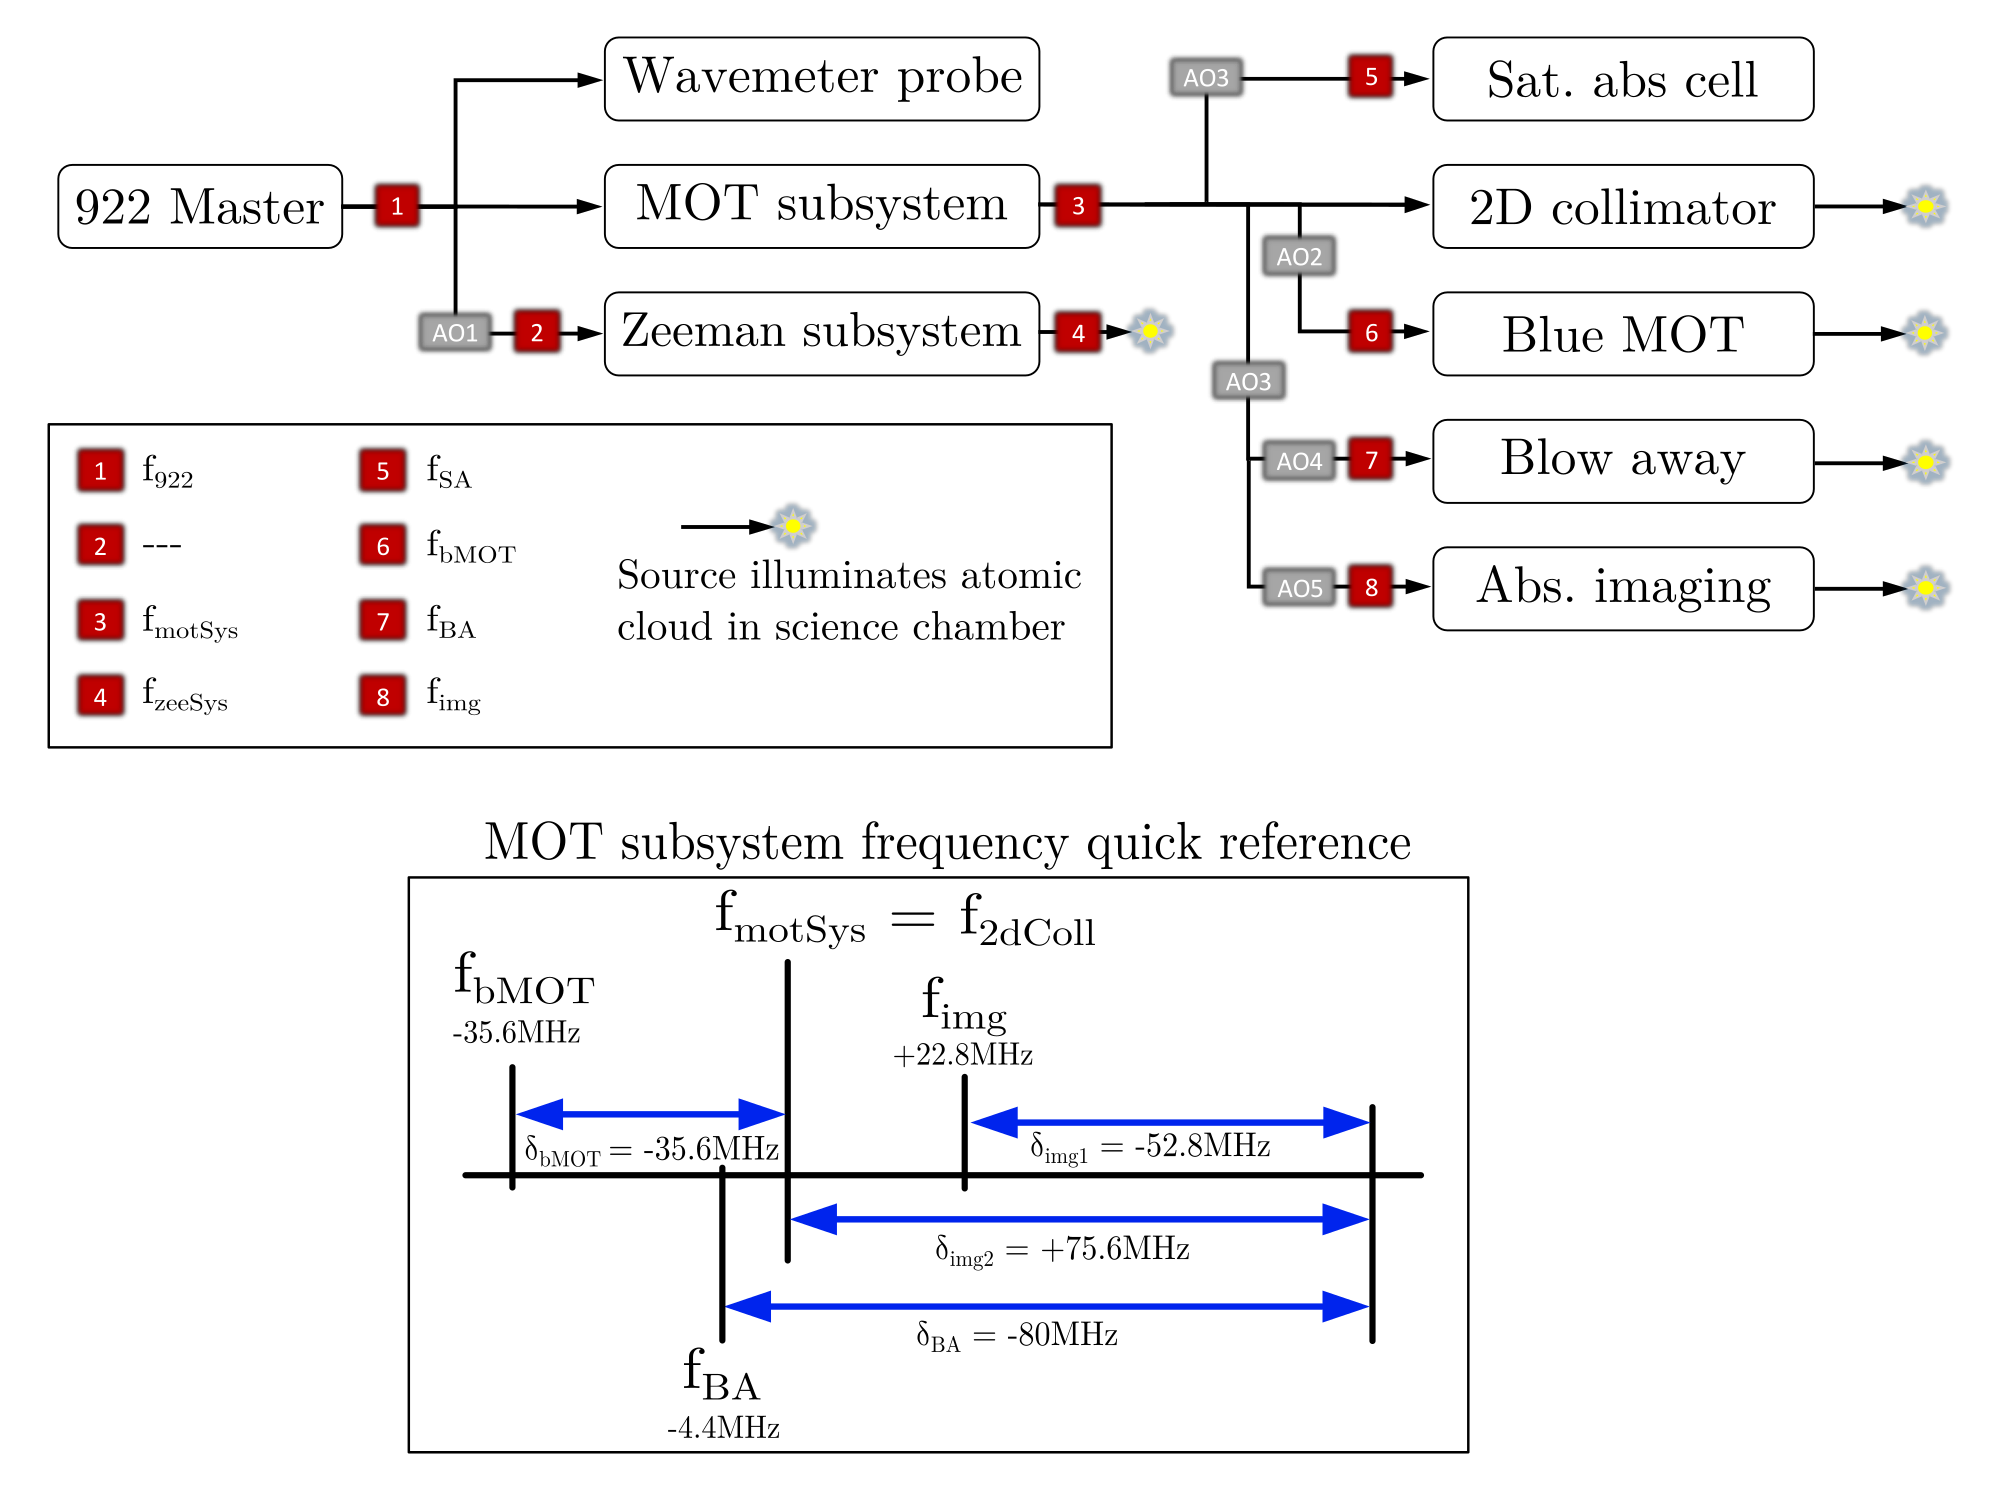
\includegraphics[width=\textwidth]{461_blueSystem.png}}
		\caption{461\,nm light generation system}{Top - Block schematic showing the relations of the various systems, AOMs, and frequencies used to lock the system for 461\,nm trapping and spectroscopy. See Table \ref{tab:461AOM} for information on the AOMs. Bottom - Relative frequencies of the MOT subsystem at various stages of the 461 system. Frequencies are quoted with respect to f$_{\text{motSys}}$ which in turn is controlled via the tunable sat. abs. to address different isotopes.}
		\label{fig:461blockSys}
	\end{figure} 

In conjunction with the block diagram, Table \ref{tab:461AOM} shows the details of the frequency shifts and AOM details. 
The position of these AOMs is represented by the numbered black circles while the labeled red squares define the various system frequencies.
The primary frequency relations for trapping and imaging are schematically represented in the lower portion of Fig.\,\ref{fig:461blockSys} and are determined via Eq. \ref{eq:461freqs}.
Table \ref{tab:461AOM} defines the shift variables used in these equations.
\begin{landscape}
\begin{table}[]
\centerline{
\begin{tabular}{@{}|l|c|c|c|c|l|l|l|@{}}
\toprule
\multicolumn{1}{|c|}{\textbf{Label}} & \textbf{Ind.} & \textbf{System} & \textbf{\begin{tabular}[c]{@{}c@{}}Shift\\ variable\end{tabular}} & \textbf{\begin{tabular}[c]{@{}c@{}}Nominal \\ Freq. {[}MHz{]}\end{tabular}} & \multicolumn{1}{c|}{\textbf{Freq. Source}} & \multicolumn{1}{c|}{\textbf{Freq. control}} & \multicolumn{1}{c|}{\textbf{AOM Model}} \\ \midrule
Zeeman & AO1 & 922 master & $\delta_{zeeman}$ & -252.4 & \begin{tabular}[c]{@{}l@{}}Mini Circuits\\ ZOS-300\end{tabular} & Static voltage & \begin{tabular}[c]{@{}l@{}}Crystal Tech. \\ 3200-1113\end{tabular} \\ \midrule
Blue MOT & AO2 & MOT & $\delta_{bMOT}$ & -35.5 & \begin{tabular}[c]{@{}l@{}}Mini Circuits\\ ZOS-50\end{tabular} & Static voltage & \begin{tabular}[c]{@{}l@{}}IntraAction \\ AOM-402A1\end{tabular} \\ \midrule
Image 2 & AO3 & \begin{tabular}[c]{@{}c@{}}Abs. imaging\\ \& Blow away\end{tabular} & $\delta_{img2}$ & +75.6 & \begin{tabular}[c]{@{}l@{}}Mini Circuits\\ ZOS-75+\end{tabular} & Static voltage & \begin{tabular}[c]{@{}l@{}}IntraAction \\ ATM-1001A1\end{tabular} \\ \midrule
Image 1 & AO4 & Abs. imaging & $\delta_{img1}$ & -52.8 & \begin{tabular}[c]{@{}l@{}}Mini Circuits \\ ZOS-150\end{tabular} & Static voltage & \begin{tabular}[c]{@{}l@{}}IntraAction \\ AOM-602A1\end{tabular} \\ \midrule
Blow away pulser & AO5 & Blow away & $\delta_{BA}$ & -80 & \begin{tabular}[c]{@{}l@{}}IntraAction \\ ME-801T7\end{tabular} & Internal synth. & \begin{tabular}[c]{@{}l@{}}IntraAction \\ ATM-802DA1\end{tabular} \\ \midrule
Sat. abs. shifter & AO6 & Sat. abs & $\delta_{SA}$ & +317.3 & \begin{tabular}[c]{@{}l@{}}Mini Circuits \\ ZOS-400+\end{tabular} & Static voltage & \begin{tabular}[c]{@{}l@{}}Crystal Tech. \\ 3200-141\end{tabular} \\ \bottomrule
\end{tabular}
}
\caption{461\,nm systen AOM details}{Ind. labels the AOMs as shown in Fig.\,\ref{fig:461blockSys}. The sign of the nominal freq. indicates the AOM order used.}
\label{tab:461AOM}
\end{table}
\end{landscape}

\begin{align} \label{eq:461freqs}
	&f_{\text{motSys}}  = 2f_{922}          & &f_{\text{zeeSys}}  = 2(f_{922} + \delta_{\text{zeeman}}) \nonumber \\
	&f_{\text{2dColl}}  = f_{\text{motSys}} & &f_{\text{bMOT}}    = f_{\text{motSys}} + \delta_{\text{bMOT}} \nonumber \\
	&f_{\text{img}}     = f_{\text{motSys}} + \delta_{\text{img2}} + \delta_{\text{img1}} & &f_{\text{SA}} = f_{\text{motSys}} + \delta_{\text{SA}} \nonumber \\
	&f_{\text{BA}}      = f_{\text{motSys}} + \delta_{\text{img2}} + \delta_{\text{BA}}
\end{align}

Overall frequency control, $f_{922}$, is determined via the magnetically tunable saturated absorption cell.
The use of magnetic tunability to control the 461\,nm light frequency is well documented in section 2.2.1 of Natali's thesis \cite{MartinezdeEscolar2010} and section 2.1.1 of Pascal's thesis \cite{Mickelson2010b}.
A more recent undergraduate project also explored optimizations of this scheme for the Rydberg apparatus \cite{MichaelViray2014}.

\subsubsection{922\,nm master}
The master 922 laser is derived from Sacher Lynx 922\,nm IR diode laser in a Littrow ECDL configuration.
Fig.\,\ref{fig:922optical}, shows a simplified optical schematic and Table \hl{some} gives typical running characteristics.
	\begin{figure}
		\centerline{
		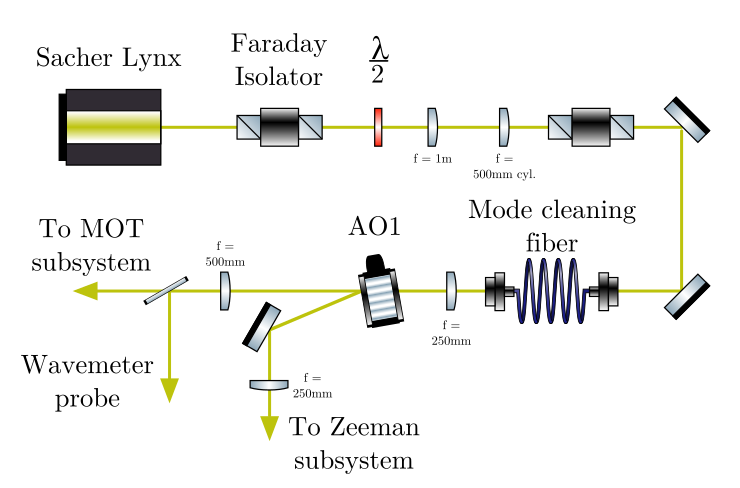
\includegraphics[width=\textwidth]{461_922schematic.png}}
		\caption{922\,nm master optical schematic}
		\label{fig:922optical}
	\end{figure} 
	
Starting at the master output, the beam is shaped and sent through a two optical isolators before it is coupled into an optical fiber.
The fiber output immediately goes through an AOM which detunes the diffracted order by approx. 250 MHz.
The diffracted and zeroth order are then separated with the unshifted beam sent towards the MOT generation subsystem and the shifted light towards the Zeeman subsystem.
We find it necessary to include dual isolators in front of the master laser and have found that inadequate alignment of these isolators can lead to significant instability in the frequency of the master which in turn may lead the doubling cavities to be unable to maintain a lock.

Fig.\,\ref{fig:922cavityLock} shows a simplified schematic of the negative feedback path for stabilizing the length of the doubling cavities.
	\begin{figure}
		\centerline{
		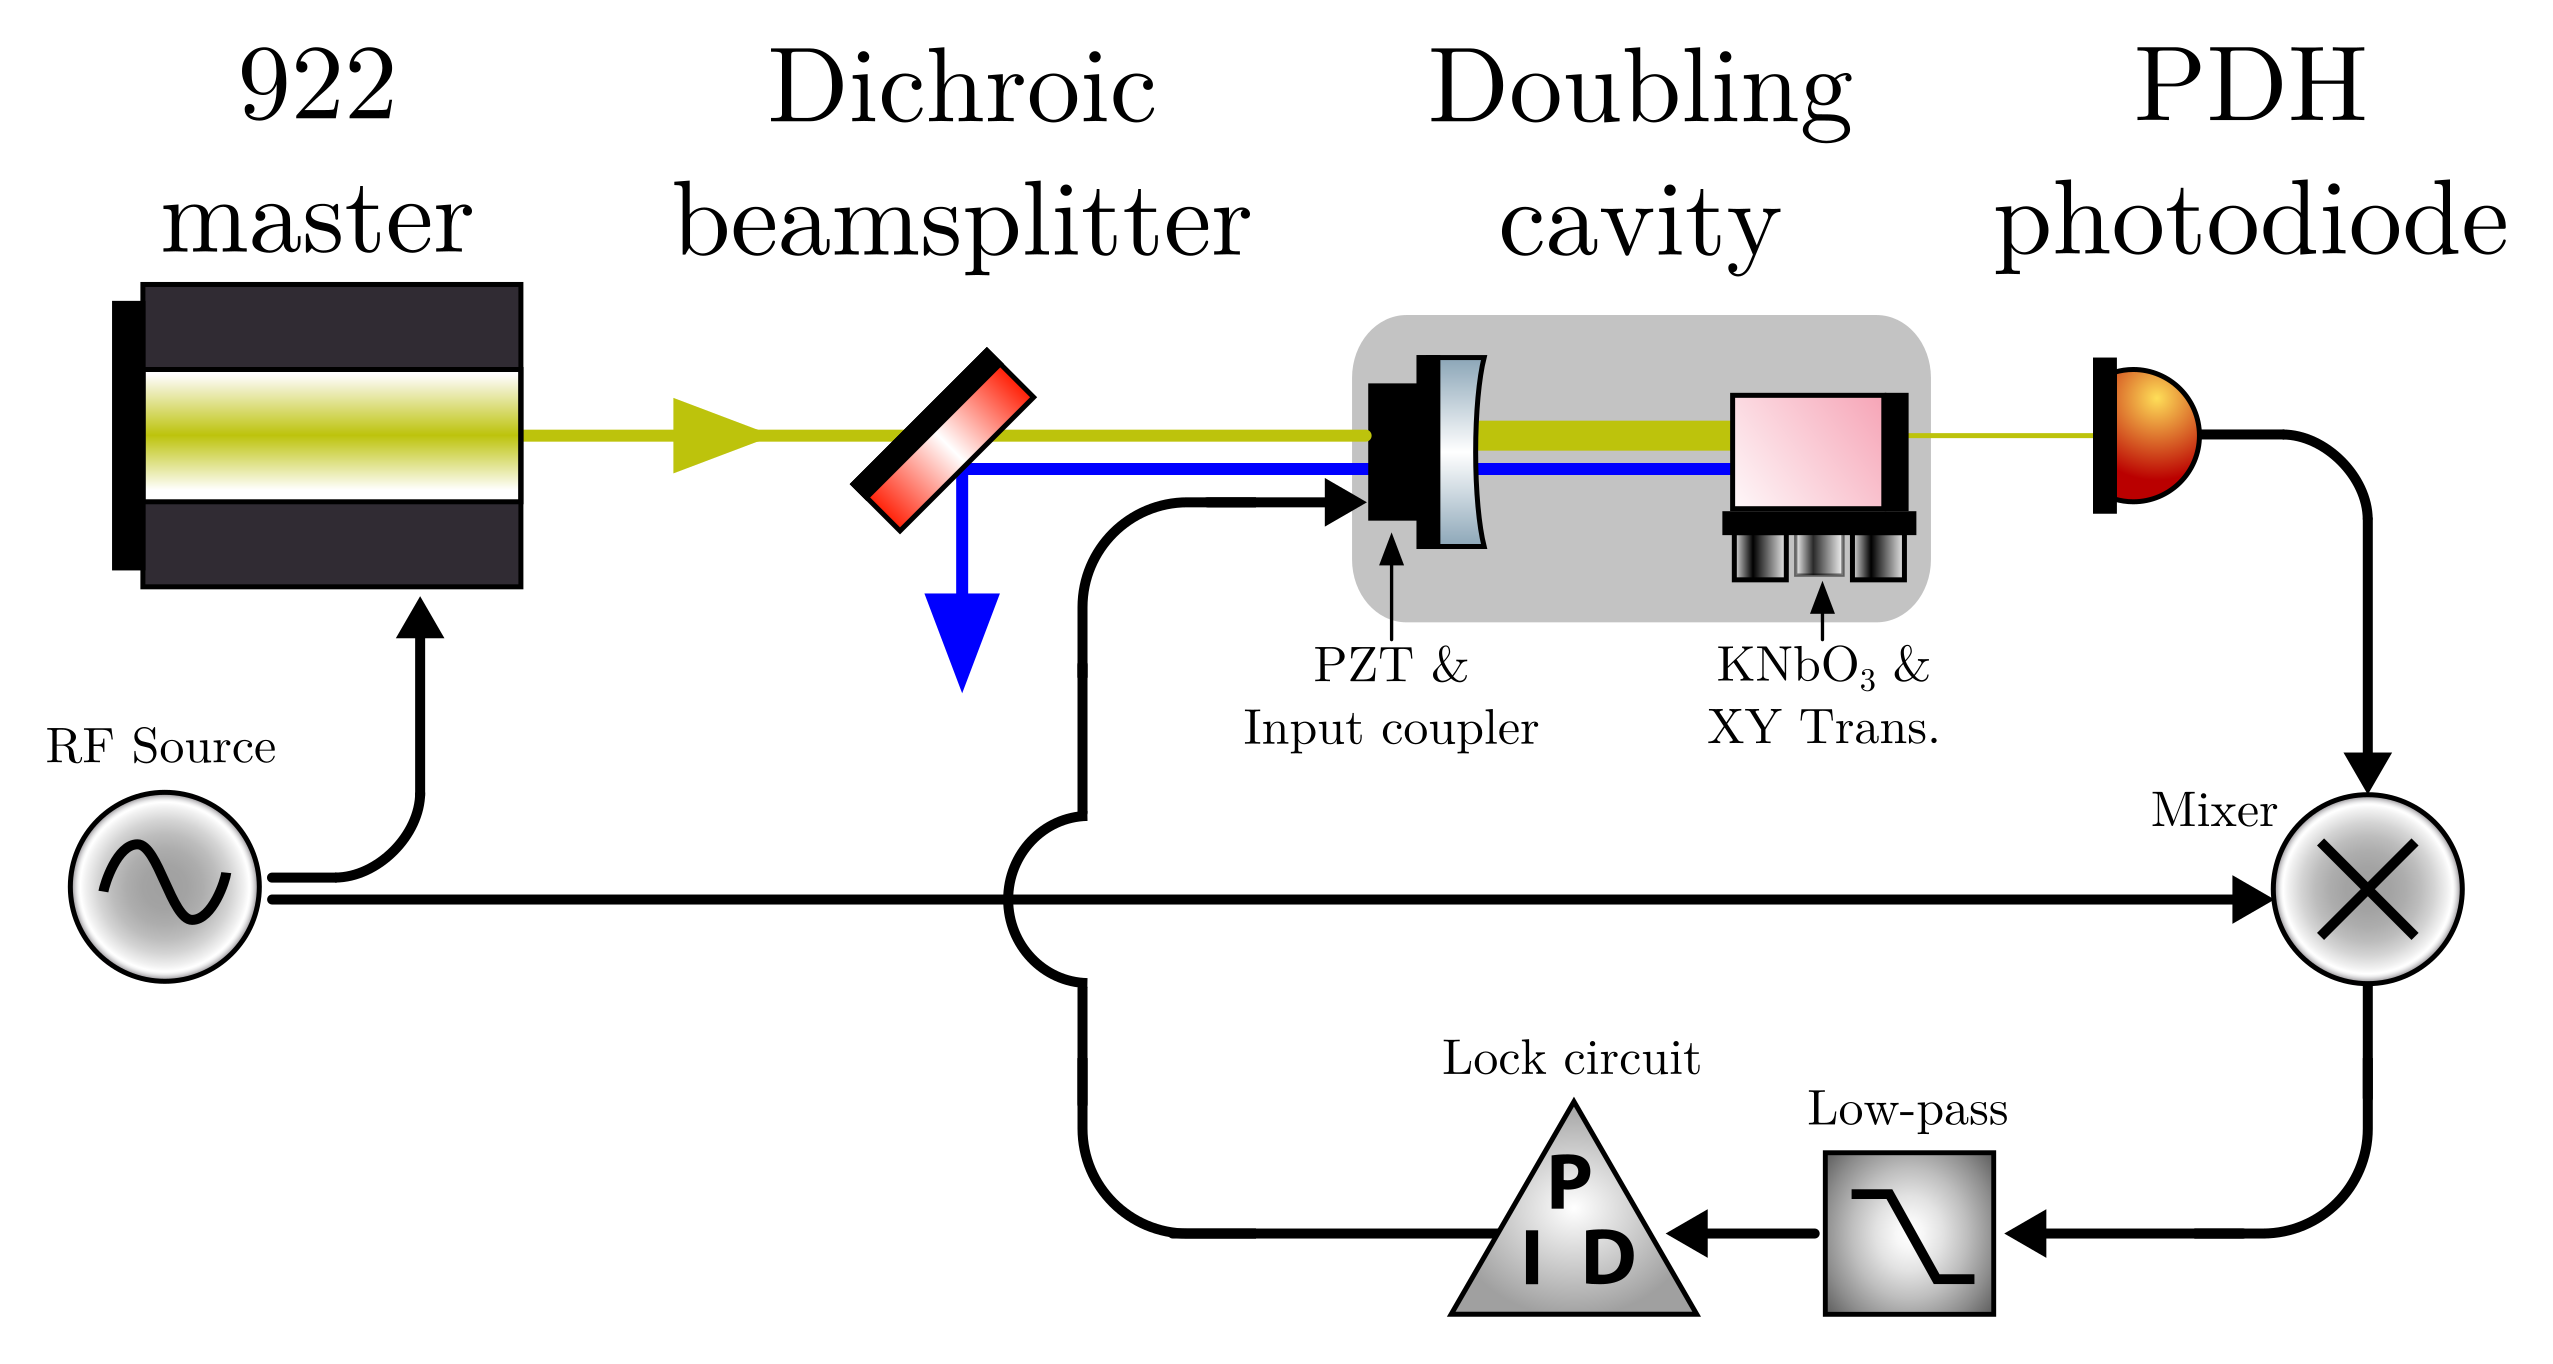
\includegraphics[width=\textwidth]{461cavitystabilization.png}}
		\caption{922\,nm doubling cavity length stabilization feedback diagram}
		\label{fig:461cavityLock}
	\end{figure}
Light out of the 922 master has sidebands added via a high bandwidth AC coupled current modulation directly to the laser diode 
\footnote{This direct coupling means the RF must be turned on prior to enabling the DC current. 
Conversely, the DC current should be disabled before turning off the RF source. 
Failure to follow this order may result in destruction of the laser diode.}.
The doubling cavities of the MOT and Zeeman sub-systems are length stabilized via these sidebands using the Pound-Drever-Hall (PDH) technique \hl{refs}.
Currently, the reference oscillator RF source is a PTS 160 from Programmed Test Sources with an output power of 12 dbm and frequency of 39.55 MHz.
This RF is sent to a 3-way power splitter (model: Mini Circuits ZSC-3-1) which sends roughly a third of the power ($\sim$ 4 dbm) to each of the MOT and Zeeman PDH mixers for demodulation. 
The remaining third is attentuated by 3db before coupling directly to the laser diode.

Once 461\,nm light is available, we stabilize the frequency of the 922\,nm using light from the MOT sub-system to interrogate a strontium heat pipe via frequency modulated Doppler-free saturated absorption from which an error signal of the $^1S_0\,\rightarrow\,^1P_1$ transition is derived.
As shown in Fig.\,\ref{fig:922freqLock}, this error signal is sent into a homemade integrator circuit with a fast feedback path controlling the 922\,nm diode current and a super low-bandwidth\footnote{This super low-bandwidth lock is based on an Arduino PID controller with a low time constant and was built by Josh Hill.
We refer the interested reader to Josh's forthcoming thesis for details of this general purpose slow lock.} 
path controlling for long term frequency drifts via the ECDL's internal PZT.
	\begin{figure}
		\centerline{
		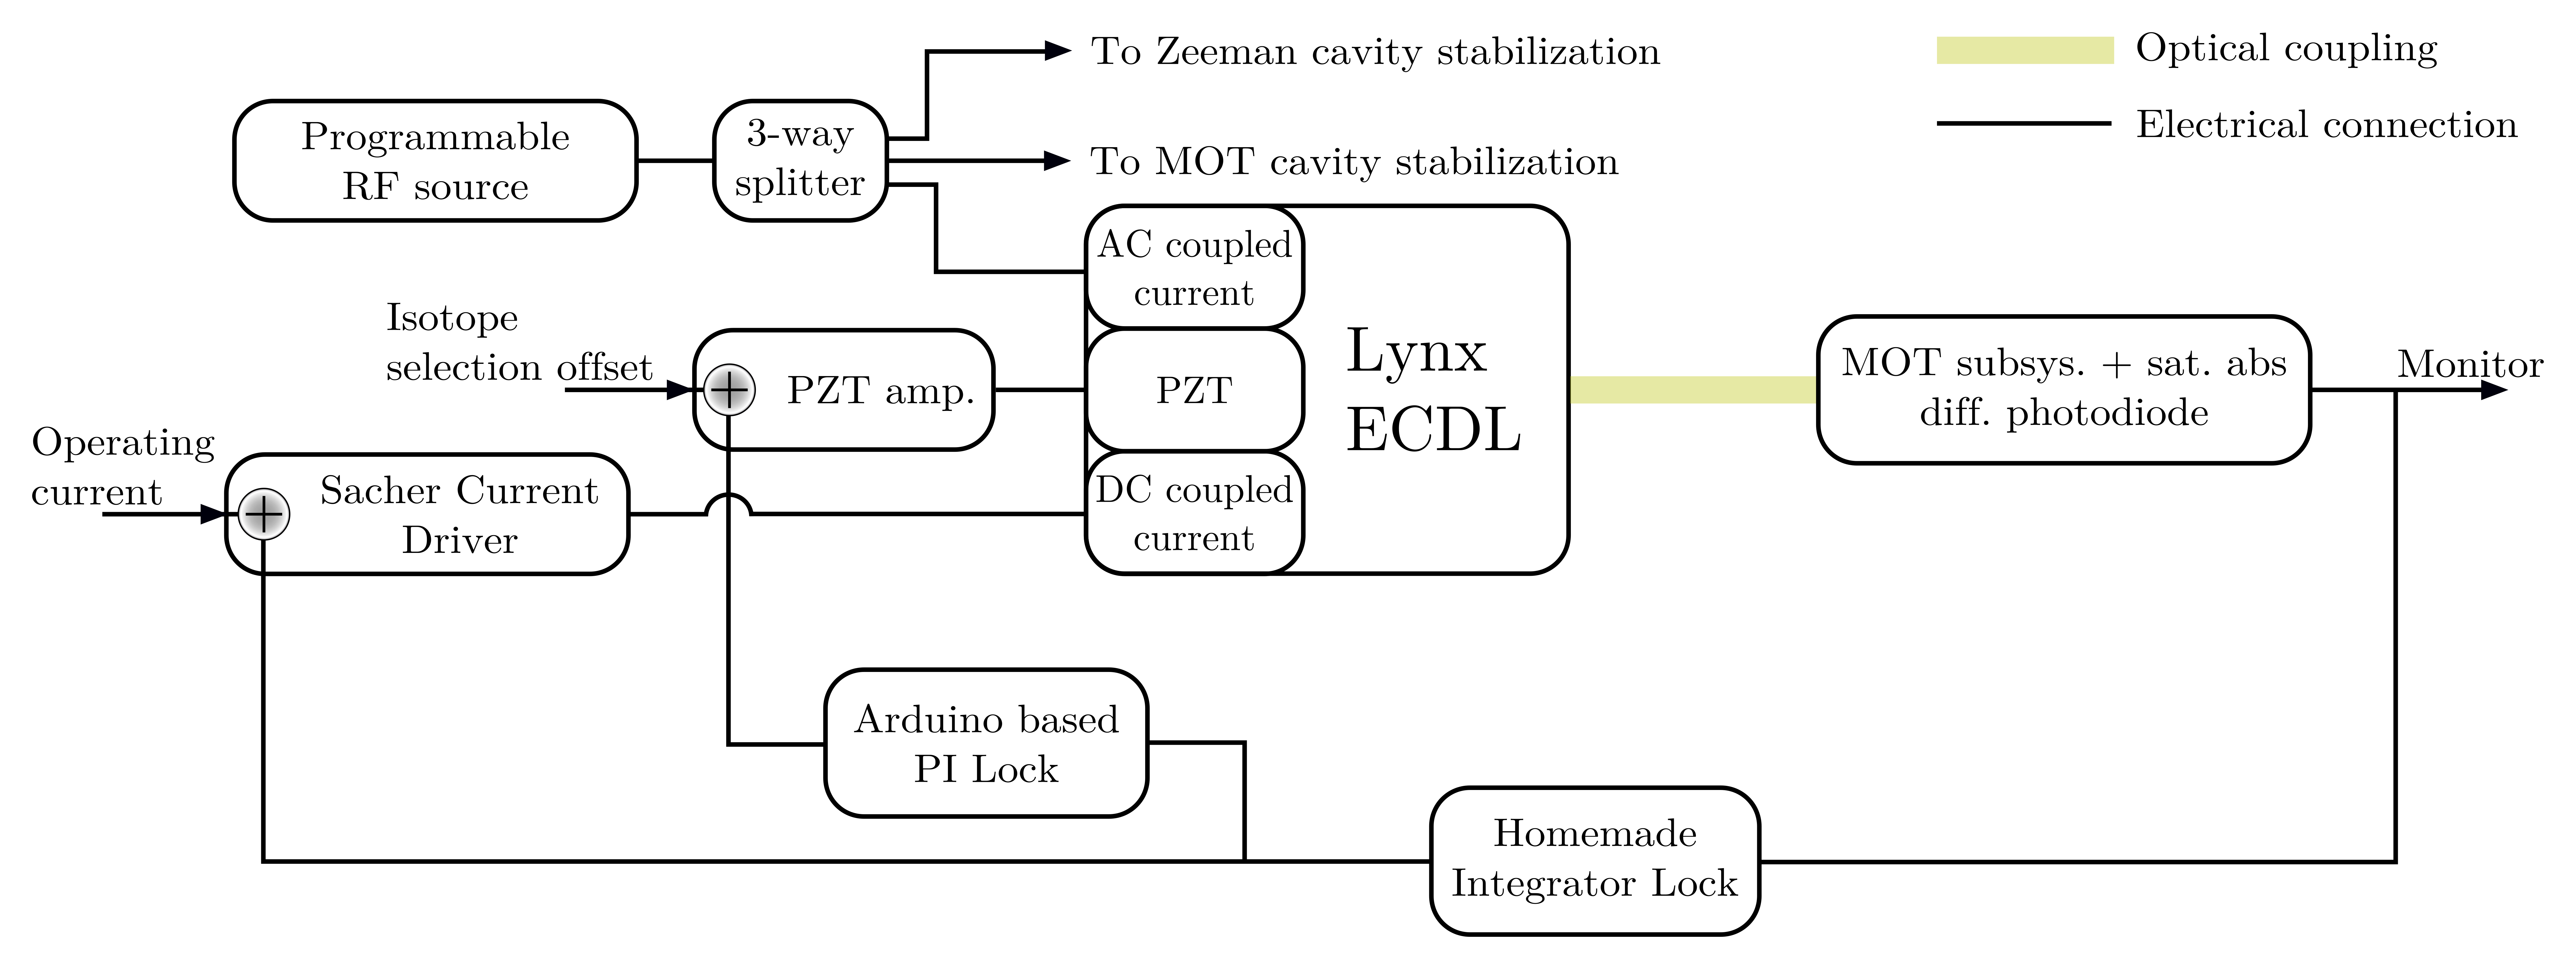
\includegraphics[width=\textwidth]{461_922feedback.png}}
		\caption{922\,nm frequency stabilization block diagram}{Multiple feedback paths allow for controlling the 922 master across disparate timescales. Note that the generation of the error signal used in the feedback is optically connected to the 922 master via the MOT subsystem and sat. abs. setup discussed in Sec.\,\ref{sec:motsubsystem}.}
		\label{fig:922freqLock}
	\end{figure} 
We found that addition of this super low-bandwidth lock has significantly improved the continuous lock time of the 461 system. 
When enabled, the experiment may stay locked for upwards of 24 hours at a time. 
As expected, such an increase in stability has greatly improved our ability to take data over long periods.
Additional details on the original construction of the 922\,nm system can be found in App. A.8 of Natali's thesis \cite{MartinezdeEscolar2010}.

\paragraph{Historical notes and tips for usage}
\subparagraph{PZT driver and replacement:}
The PZT driver provided by Sacher has become problematic over the laser few years.
When varying the voltage we would occasionally hear a "clicking" noise from the Lynx laser as if the voltage was abruptly changing.
We moved to a Thorlabs analog PZT driver (model: MDT694A) and have not had this issue since the switch.
Note that the maximum voltage for the Sacher PZT is 100 V so the driver should be limited accordingly.
Additionally, we attempted to use the newer Thorlabs MDT694B which incorporates an enable control on the voltage knob via a digital potentiometer instead of the analog pot of the "A" model.
However, we quickly abandoned the "B" model as the resolution of the digitization caused the laser frequency to jump large amounts and we were unable to maintain the frequency lock.

In early 2017, we found that the Lynx PZT was no longer responding to applied voltage.
We believe this was caused by the afore mentioned "clicking" issue and was the motivation for changing PZT drivers.
Details and pictures of the PZT replacement are available in App. \hl{something}.

\subparagraph{Sacher temperature setpoint:}
Unfortunately, the woes of the Sacher equipment have not been limited to their PZT controller.
Great care must be taken when attempting to change the set temperature of the laser diode as it seems that the internal potentiometer does not maintain full contact such that when attempting to turn it ever so slightly the set point temperature may jump from approx 16 \degreeC to 11 \degreeC.
Worse yet, we have observed that after changing the temperature there is a settling time during which the temperature setpoint may change while not be monitored.
For these reasons we generally avoid touching this control as the present setpoint of 16.1 \degreeC is adequate and no major improvements have been found when changing this temperature.

\subparagraph{Daily alignment:}
The input coupler for the 922 cleanup fiber is not a reliable mount and tends to drift significantly from day-to-day.
Therefore, we find it useful to peak up the alignment into this fiber while monitoring the output power at a fixed position after the fiber.
Importantly, the positioning of the power meter head seems to effect the amount of power measured by the device (especially as the head ages).
Thus, we use optical mounts in an attempt to reproduce the spatial position everyday and typically acheive a coupling efficeincy of $\sim$51\% through the fiber.
See Sec. \ref{sec:dailyStats} for more details.
		
\subsubsection{Zeeman subsystem}
The Zeeman sub-system is a dedicated TA + doubling cavity for generating approx. 125 mW of 461\,nm light exclusively used for the one-dimensional Zeeman cooling stage.
%There are numerous works exploring the construction and optimization of Zeeman coolers for use with strontium \hl{genetic ref, francy ref, others?}.
This system was originally constructed by Aaron Saenz \cite{AaronDSaenz2005} with additional details available in App A.8 of Natali's thesis \cite{MartinezdeEscolar2010}.
Figure \hl{something} shows a simplified optical schematic of this system.
	\begin{figure} 
		\centerline{
		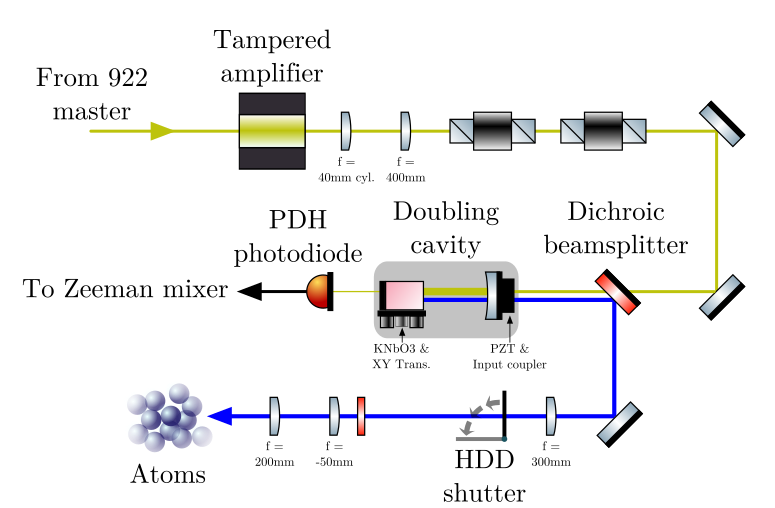
\includegraphics[height=0.4\textheight]{461_zeemanSubsystem.png}}
		\caption{Zeeman subsystem optical schematic}
		\label{fig:zeemanSchematic}
	\end{figure}
Light from the 922 master (approx. 20 mW) is shaped and coupled into a tapered amplifier to produce nearly 300 mW of 922\,nm light.
After being shaped further and passed through dual isolators, the light is then coupled into the homemade doubling cavity where a potassium niobate crystal is held within an optical resonance cavity to produce the 461\,nm light.
For approx. 300 mW into the cavity we are able to produce approx. 125 mW of 461\,nm light.
This light is sent through a final beam expander and into the chamber where we have designed the system to focus the Zeeman beam just at the tip of the atom nozzle to maximize the spatial and temporal interaction between hot atoms and the Zeeman beam.
Table \hl{something} provides typical running characteristics of the system \hl{note thermistor in table}

\paragraph{Historical notes and tips for usage}
\subparagraph{Mode hop:} 
Doubling cavities at such short wavelengths are known to be mercurial \hl{aaron refs} so stabilizing them can be difficult. 
We find that this cavity tends to become stable with \hl{whatever the input power is} as increases of the input power beyond this result in an initial cavity lock producing more 461\,nm light but which quickly mode hops into a lower power mode.
While we have seen cavity output powers of up to 150+ mW, these are not stable modes.
Additionally, the locking circuit contains an auto re-lock feature that can occasionally result in locking to a lower power mode, usually around $\sim$80 mW.
We have found that power cycling the TA current driver is the least intrusive and typically successful method to reattain the 125 mW output.
If cycling does not work, then the TA current output may need to be adjusted.

%\subparagraph{Beam quality:}
%Great care has been taken to minimize any structure present on the 461\,nm Zeeman beam in order to maximize the amount of stopping force which can be derived from this beam.
%Fig. \ref{fig:461zeemanBeam} shows the Zeeman beam just before entering the chamber.
%The cause of the intensity asymmetry which can be seen to the right is unknown, but has been confirmed to be present even directly out of the doubling cavity.
%	\begin{figure}
%		\centerline{
%		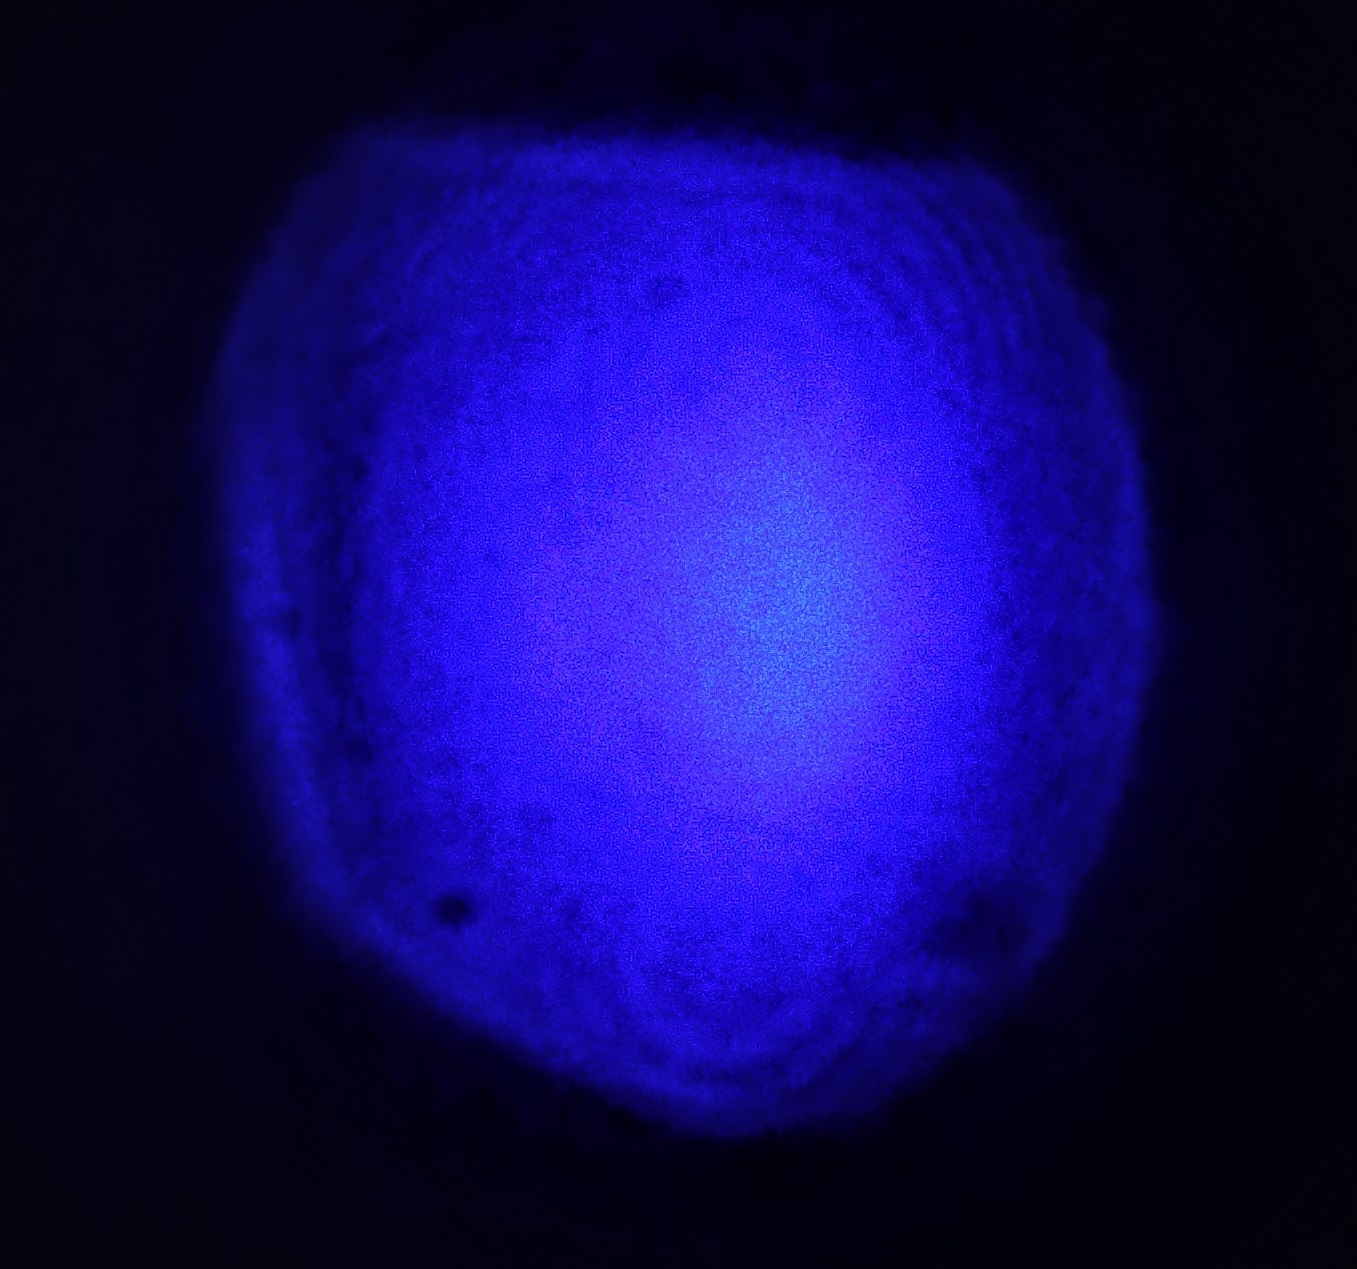
\includegraphics[height=0.25\textheight]{461_IMG_20171213_13048.jpg}}
%		\caption{Characteristic beam quality of the Zeeman laser}
%		\label{fig:461zeemanBeam}
%	\end{figure}
%	
%	Zeeman TA
%		Components
%			Mounts
%			Optics
%			Circuits
%				current control board
%				temp control board
%					note the thermistor in use
%		Typical running values
%			in power
%			out power
%			TA current
%			TA temp
%		
%	Cavity
%		Components
%			Optics
%		Typical running
		
\subsubsection{MOT subsystem} \label{sec:motsubsystem}
The MOT path generates light used for a multitude of processes as shown in Fig \ref{fig:461blockSys}.
Here we detail the systems required for laser cooling and trapping, leaving the details of the blow away pulser and absorption imaging to be discussed in Sec. \ref{ssec:op_tools}.
Furthermore, we begin our discussion wih a focus on the light generation of the MOT subsystem and next we will explore the child setups derived from this subsystem.

Fig.\,\ref{fig:motSchematic} shows a simplified optical schematic of the MOT subsystem which is modeled after the Zeeman setup described previously.
Light from the 922\,nm is shaped, amplified, and coupled into the doubling cavity where the same feedback mechanism shown in Fig.\,\ref{fig:922cavityLock} is used to stabilize the cavity length.
	\begin{figure} 
		\centerline{
		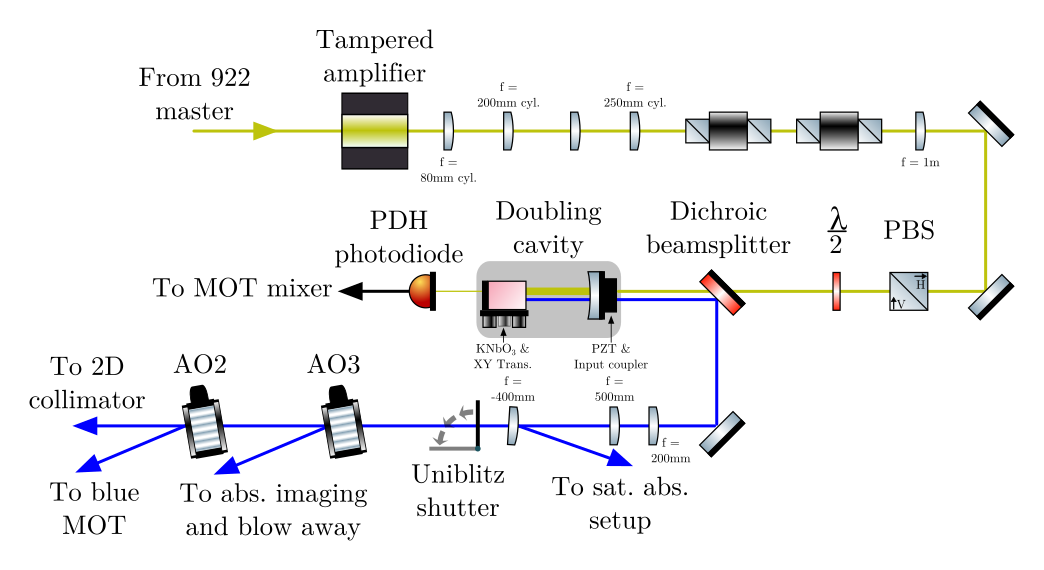
\includegraphics[width=\textwidth]{461_motSubsystem.png}}
		\caption{MOT subsystem optical schematic}{Note the sharing of power between the 2D collimator and blue MOT paths. While the blue MOT is power stabilized as shown in Fig.\,\ref{fig:blueMOTSchematic} the 2D collimator utilizes the remaining laser power.}
		\label{fig:motSchematic}
	\end{figure}
Since the MOT system is situated close to the experimental chamber, a "black-house" wall and shroud were constructed to minimize stray reflections.
This enclosure was placed around the MOT subsystem to mitigate stray 461\,nm light which can significantly hinder the achievement of quantum degenerate strontium gases.
\footnote{Even stray reflected light off the glossy ceiling of the experimental enclosure has been found to cause atom heating!}
Part of this enclosure is a fast ($\sim$2 ms) shutter (model: Uniblitz CS45) used to block the 461\,nm light during the red MOT and evaporation stages.
Additional hard drive (HDD) shutters are also placed along the MOT path behind the black-house shutter as leakage light through the blue MOT AOM (AO2) specifically was seen to cause additional heating when utilizing the blow away pulser.

One concern we face with this MOT setup is the coupling of power between the various paths.
Typically we do not operate the imaging \& blow away pulser while trapping so all available power from the doubling cavity is available for these processes.
However, the 2D collimator and 461\,nm MOT operate concurrently during the first stages of trapping so the available laser power must be split between these two systems and thus an equilibrium must be found which balances the optimum trapping force and the optical molasses of the collimator.
We have observed the 2D collimator to increase the number of trapped atoms in the 461\,nm MOT by about a 7x factor when operating optimally.

\paragraph{461\,nm MOT}
Fig.\,\ref{fig:blueMOTSchematic} gives an overview of the 461\,nm MOT optics\footnote{The MOT arms are labeled as they are organized on the table, where Arm B is closest to the "computer side" of the table.}.
Separation of the laser beams is performed on the table level where custom dichroics are used to combine the 461 and 689 MOT paths.
Following the dichroics, the MOT beams are directed up to the platofrm layer via periscopes and subsequently pass through dual wavelength waveplates which retard 461\,nm light by three-quarters of a period and 689\,nm by one-quarter.
This setup allows us to maintain well defined polarization along the MOT paths.
	\begin{figure} 
		\centerline{
		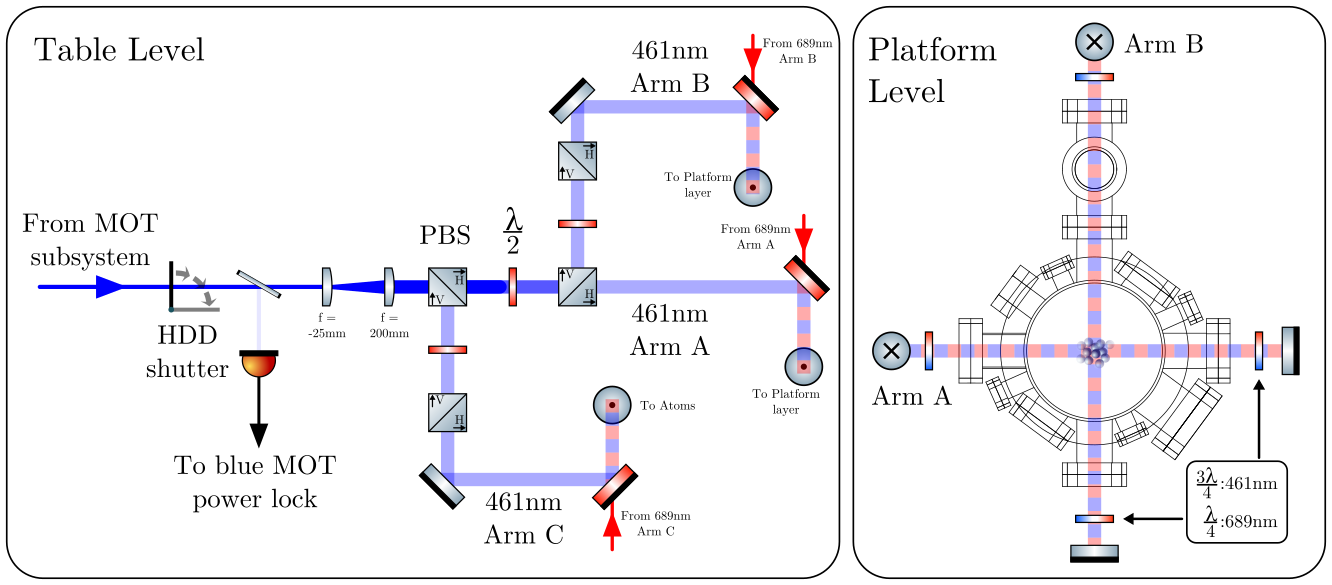
\includegraphics[height=0.4\textheight]{461_blueMOTschematic.png}}
		\caption{461\,nm MOT schematic}{Typical MOT setup with an additional HDD shutter to mitigate light leakage from AO2. Transparency of the laser beams represents the intensity. Note the 461\,nm and 689\,nm light follow the same path through the science chamber. Custom waveplates acting on both wavelengths are used to provide the appropriate polarization.}
		\label{fig:blueMOTSchematic}
	\end{figure}
Each MOT beam operates with $\sim$\hl{num}\,mW of power with a beam size $\sim 1$\,in. for a trapping intensity \hl{??}.
During MOT operation this intensity is locked via an intensity stabilization circuit.

%Characteristic power in each beam
%MOT beams are power controlled via the feedback system shown in fig.
%The custom power lock integrated circuit is given in \hl{figure in appendix}.
%This design is based off the work report by Ying Huang but with several modifcations for adding a transimpedence amplifier as the input stage.
%The power setpoint is a controlled input from the 	

\paragraph{Saturated absorption}
The saturated absorption cell is used to interrogate the $^1S_0\,\rightarrow\,^1P_1$ transition in order to lock the frequency of the 922 master.
App. \ref{app:dopSpec} outlines a brief derivation for determining the lock point when a constant offset is added to the laser frequency, as is the case here.
As outlined in the derivation, by utilizing the Zeeman tunability of magnetic sublevels, we can shift the resonance frequency of the atoms in the heat pipe.
Thus, by interrogating and locking to the transition frequency of the most abundant isotope, $^{88}$Sr, we can shift it's resonance to cover the isotope shifts of the other strontium isotopes.
This provides a simple method for trapping various isotopes and mixtures of strontium.

A detailed walkthrough of the construction and relevant physics of a blue sat. abs. cell can be found in the undergraduate report of Michael Viray \cite{MichaelViray2014}.
Additionally, the original construction of the Neutral cell is covered in section 2.2.1 of Natali's thesis.
Fig.\,\ref{fig:blueSatAbs} shows the optical setup used to generate the error signal and reference traces of Doppler bowl and frequency lock error signal.
This error signal is generated by frequency modulating the magnetic field of the cell and performing Doppler free saturated absorption.
	\begin{figure} 
		\centerline{
		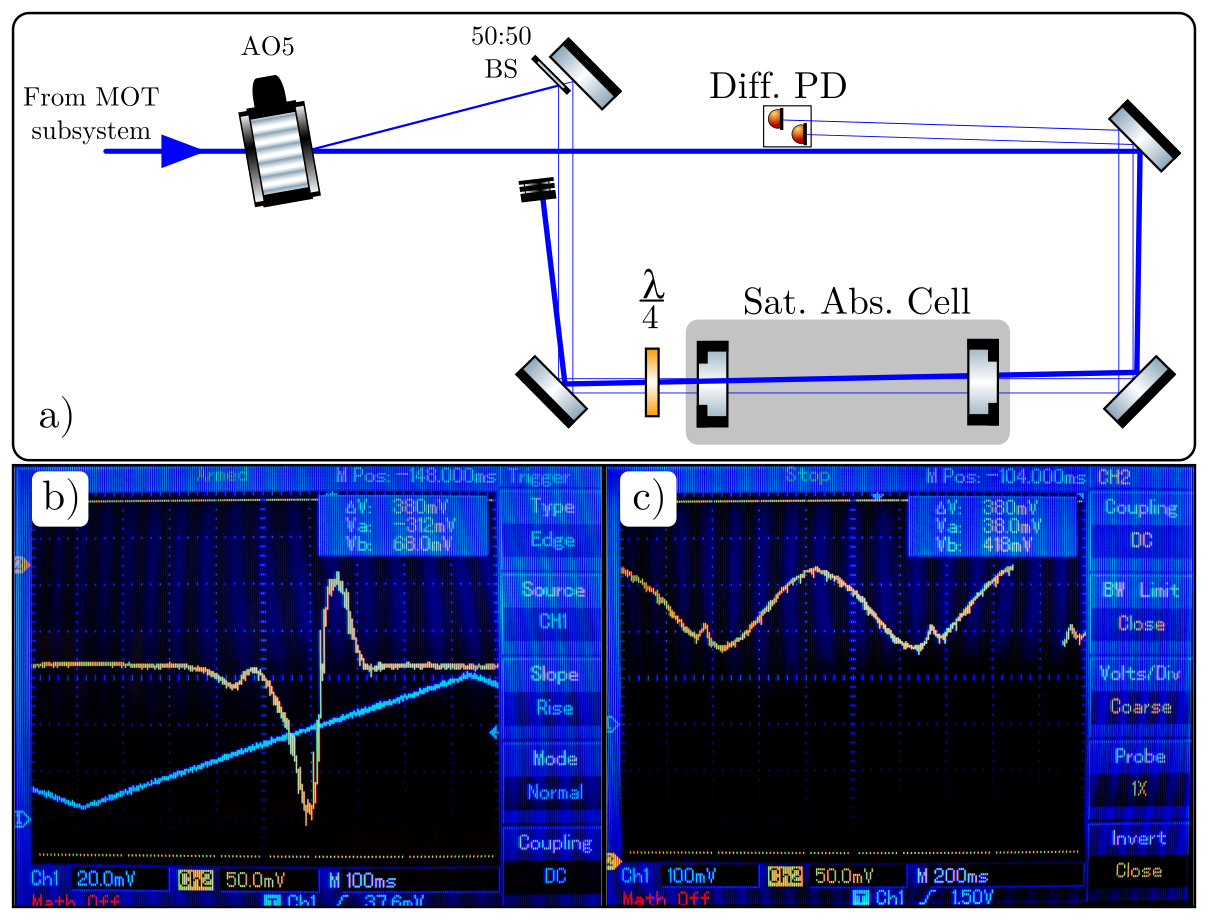
\includegraphics[width=0.7\textwidth]{461_satAbsSchematic.png}}
		\caption{461\,nm saturated absorption setup}{a) Optical setup for frequency locking the 922\,nm master. b) Example error signal. The cause of the asymmetry is unknown but occurs around approx. $\pm$1.7A drive. The offset seen here can be nulled by balancing the amplification applied to the differential photodiode inputs. c) Example of the Doppler bowl where the Lamb dip can be seen. Note that the Lamb dip interacts with a specific velocity class determined by $\delta_{SA}$.}
		\label{fig:blueSatAbs}
	\end{figure}

\paragraph{Historical notes and tips for usage}
\subparagraph{Daily alignment of MOT TA:}
The simplified optical schematic of the MOT subssytem in Fig.\,\ref{fig:motSchematic}, does not reflect the approx. two meter lever arm which is present between the Zeeman split AOM and the input to the MOT TA due to the relative positions of the cavities.
We have found this requires us to peak up the alignment of the 922 master beam into the MOT TA on a daily basis and is hypothesized to be the cause of large long time power variations ($\sim$15\%) on the output power of the MOT cavity which we observe throughout the course of the day.
Typically with an input power of approx. 300 mW of 922\,nm light we get between 100 - 115 mW out on a daily basis.

\subparagraph{Note on changing isotopes:} \label{para:change_iso}
While the basic setup has not changed over the many years, we have recently moved away from the original current source based on a home built high-current FET amplifier to a Bi-polar current source (BOP) (model: Kepco BOP-20-10DL).
This change allows for more expansive coverage of the $^1S_0\,\rightarrow\,^1P_1$ isotopes shifts. The previous current source limited our dual trapping capability to 87+88, and required an AOM to be tweaked and the sat. abs. to be realigned for trapping 84 and 86. 
Using the BOP, we can now easily shift the transition frequency over approx. $\sim$200 MHz which allows us to span the range between 84 and 87 within a single experimental cycle.
Given the geometry of our solenoid, large currents are required to apply such large Zeeman shifts.
We have observed that these large currents increase the heat load on the cell, which can lead to a reduction in the error signal.
We mitigate this additional heating by varying the heater current to maintain approx. 50\% absorption of the pump beam.
As we expect, the timescale for these effects are minutes, so short term variations (i.e. when doing spectroscopy) do not cause significant heating when the duty cycle is kept low.

Due to the heating from the Zeeman coil, we chose to balance the currents needed to trap 84 and 87 by "centering" the pump-probe beams frequency such that the magnitude of the currents needed for both isotopes is similar, but with 84 requiring a $(+)$ current and 87 a $(-)$ current.
However, trapping of 88 still requires the realignment of the sat. abs. pump-probe beams as this shift is just beyond the capabilities of the current drive. 
Care should be taken when adjusting this alignment as the paths are highly coupled as can be seen in Fig.\,\ref{fig:blueSatAbs}a).

%Simplifed optical schematic
%
%While realigning the sat. abs. is not always necessary
%
%Give calibration plot?
%
%MOT light path
%	Components
%		TA
%		Cavity
%		AOMs
%		Shutters
%	
%	MOT TA
%		Components
%			Mounts
%			Optics
%			Circuits
%				current control board
%				temp control board
%					note the thermistor in use
%		Typical running values
%			in power
%			out power
%			TA current
%			TA temp
%		
%	Cavity
%		Components
%			Optics
%		Typical running

%\subsection{Repumping: 481\,nm}
%\label{ssec:481sys}
%
%Plot from Rydberg
%
%Discuss the change with the EOM
%	Frequency center of EOM and range?
%	
%Data on picking the timescale?
%	I know I choose like 40ms (including delay, but did I take data on this)
%
%This system is based on a Toptica DL-100 littrow laser which produces about 8mW of power at 481\,nm. 
%Excitation to a doubly excited state is an eay way to do the repumping.
%As it is difficult to create and maintain a population of atoms in the $^3P_2$ state, we use a telerium oven to lock the laser.
%The original setup of this system was done by Pakorn \hl{ref} who setup a side of peak locking scheme. 
%Ten by dithering the laser current we can broaden that laser and extend to the strontium transition.
%
%Recently, we have begun to trap multiple isotopes across the different labs and have found our naive appraoch to locking the repumper to be inadequate.
%Working with the Rydberg apparatus, we performed spectroscopy of the repumping transition by counting the number of atoms which were returned to the ground sate as a function of repumping frequency.
%During these experimens we found that very small amounts of power, on the order of $\mu$W's, is needed to obtain large ground sate populations when the laser is tuned precisely to the isotopic transtion energy. 
%Fig.\,\hl{something} shows the result of this spectroscopy for multiple strontium iotopes.
%It was not feasible to dither the current across the GHz of detuning needed without mode hoping the laser so we decided to use an EOM driven at high power to place multiple orders of sidebands onto the laser light.
%
%What frequency is the EOM running at?
%What frequecnies do we aim to hit precisely?
%
%The current setup uses the EOM in addition to dithering the laser current a small amount to address these transitions.
%With this finding we decided to use an EOM to place multiple orders of sidebands on the laser light
%This allows us to address multiple transitions more precisly
%
%Optical schematic
%Light from this laser is split into five paths.
%One for each experiment, another for monitoring the wavelength, and the last for probing the tellerium transtion.
%
%Feedback diagram
%We have found
%
%\subparagraph{Historical note:}
%The lead screw, which is part of the internal alignment mechanism of the Littrow ECDL, was nearly stripped at some point when attempting to peak up the frequency stability. 
%Extreme care should therefore be taken when using this adjustment as the brass baseplate of the DL-pro is soft and there is a potential to strip out the remaining threads.
%	\begin{figure}
%		\centerline{
%		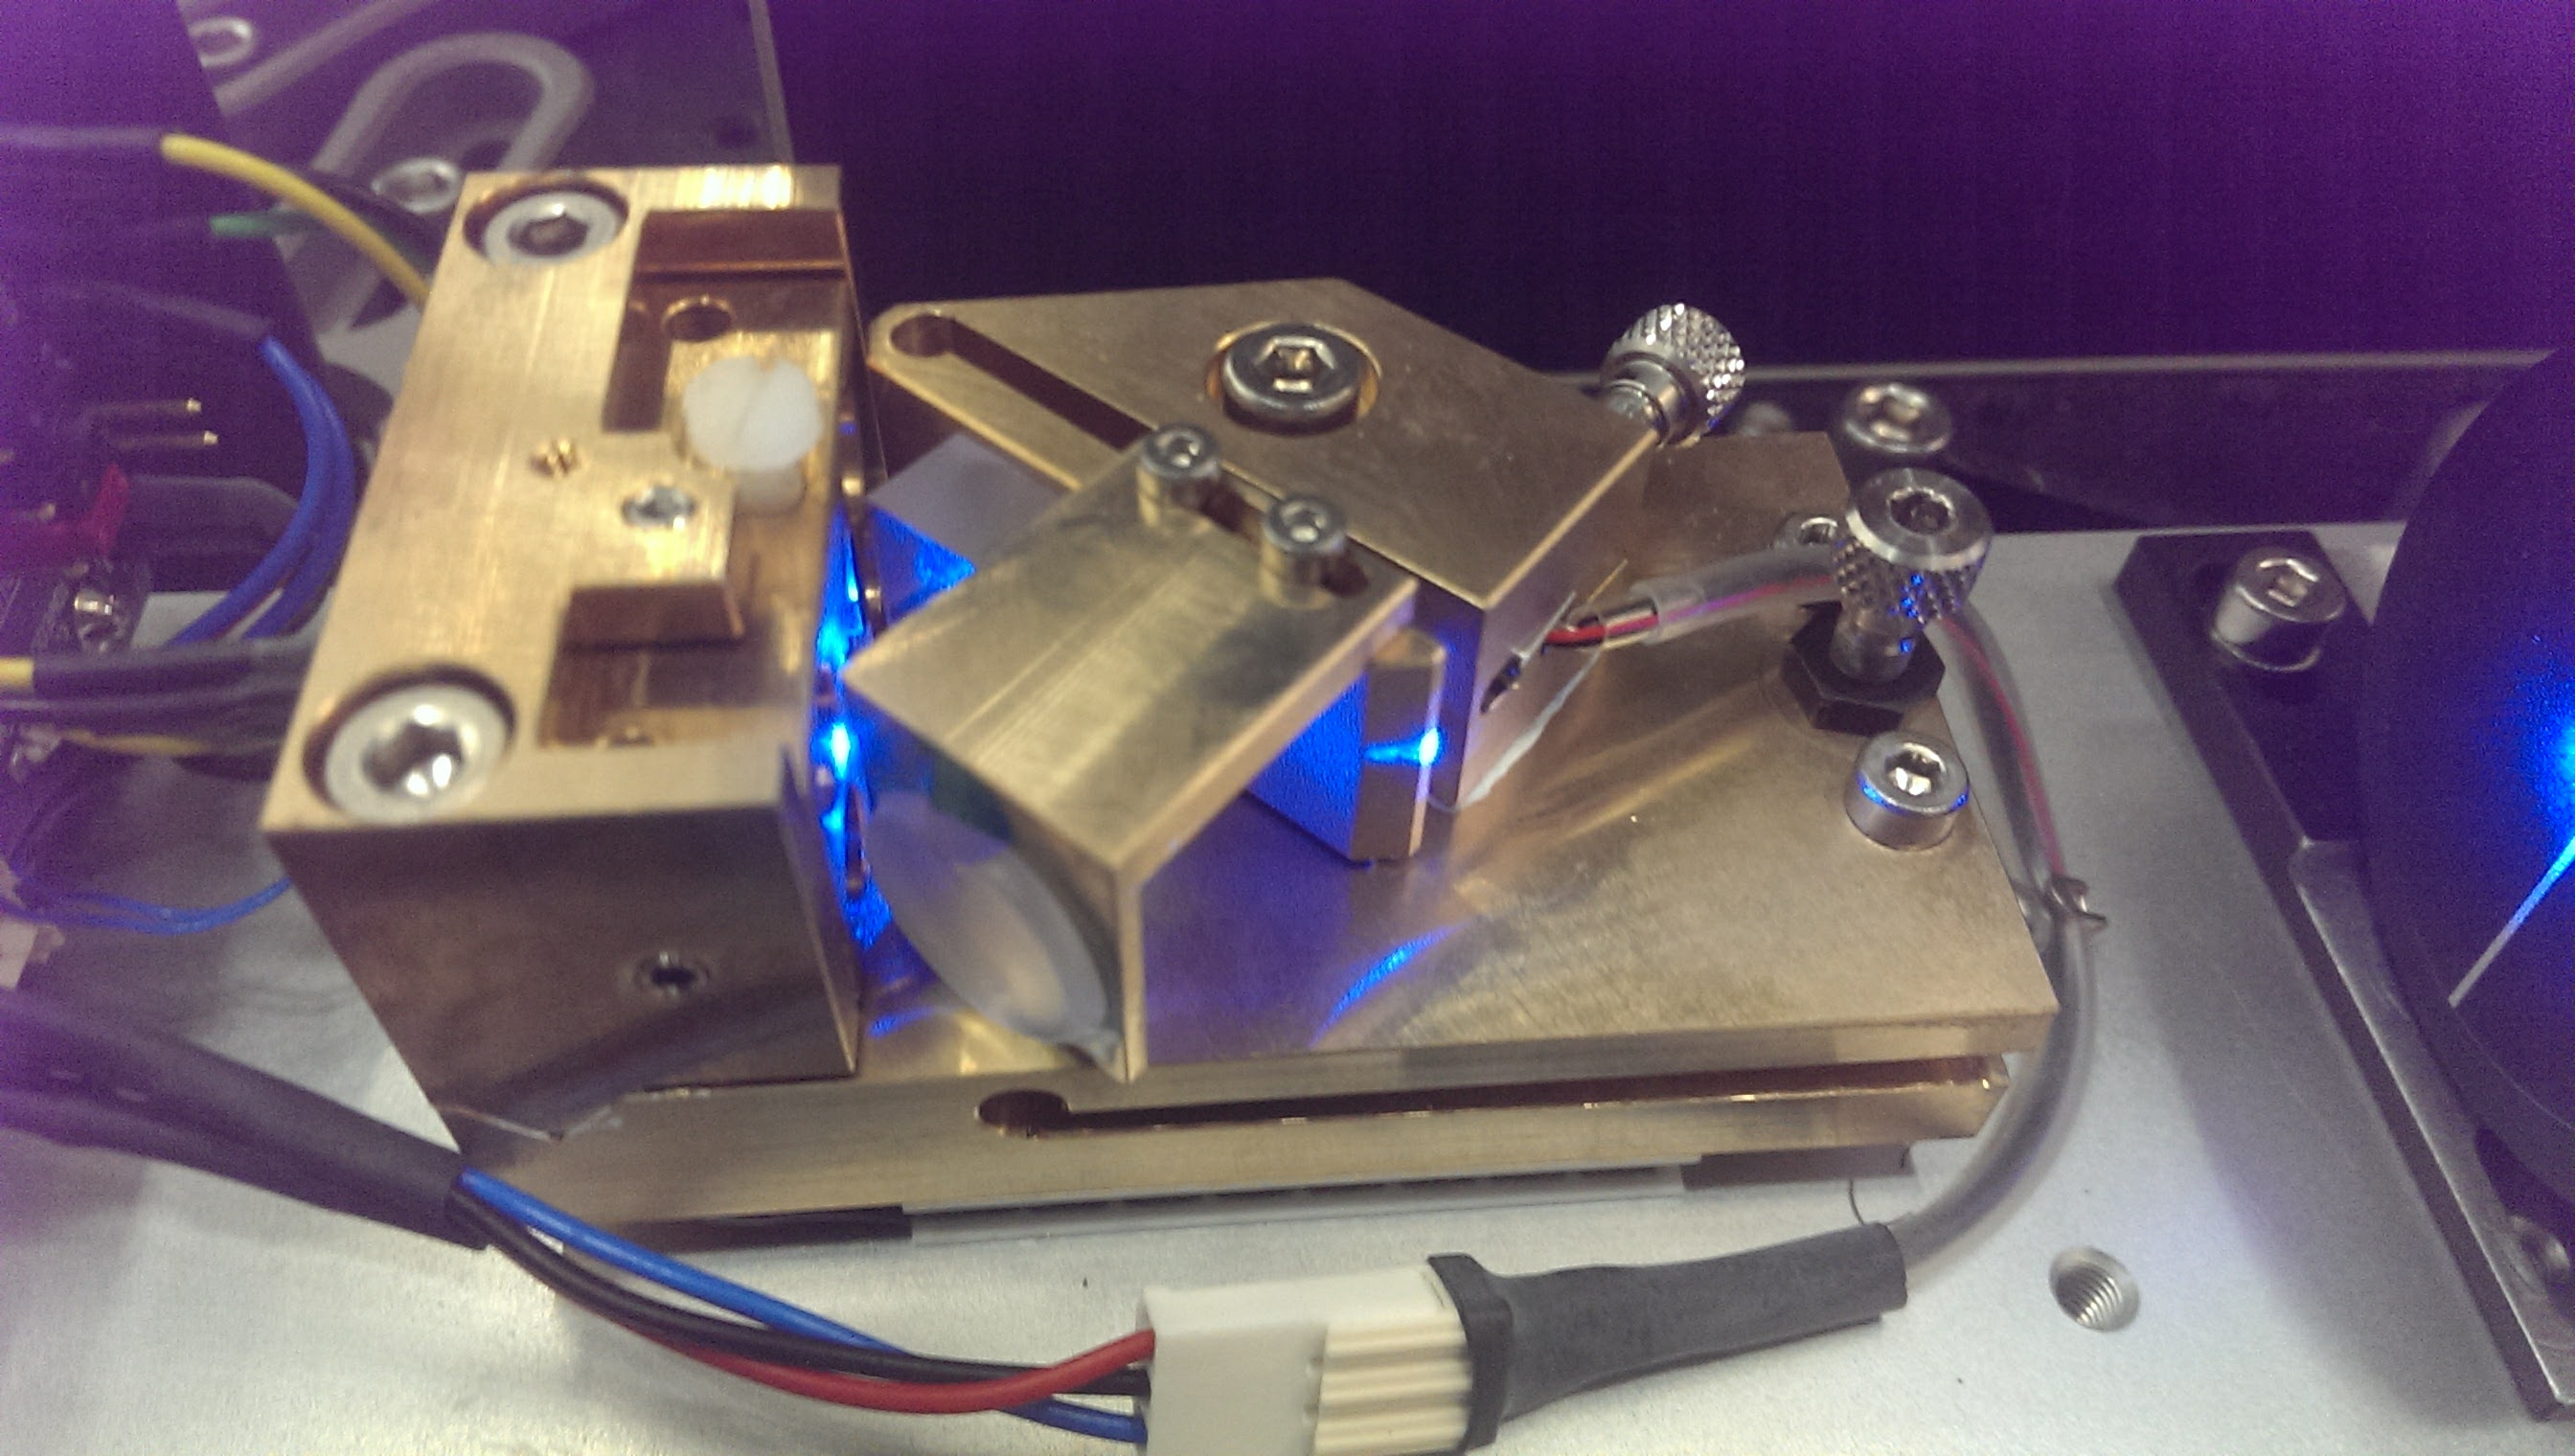
\includegraphics[height=0.2\textheight]{481_IMAG0022.jpg}}
%		\caption{Internal view of the 481\,nm ECDL}{The red box denotes the alignment screw that should be adjusted with caution.}
%		\label{fig:481internal}
%	\end{figure}

\pagebreak
\subsection{Narrowband cooling stage: 689\,nm} \label{ssec:689sys}
\subsubsection{Overview}
The work horse transition of strontium is the $^1S_0\,\rightarrow\,^3P_1$ intercombination line transition at 689\,nm. 
In addition to cooling and trapping, most experiments performed in our lab utilize this transition as our primary probe owing to the narrow linewidth which allows for high precision measurements and large detunings using conventional techniques.

Fig.\,\ref{fig:689blockSys} shows an overview of how we generate and use the 689\,nm light. 
The following section will describe the trapping portions of the red system and Sec.\,\hl{something} will explore the spectroscopy probe setup and it's various configurations.
	\begin{figure}
		\centerline{
		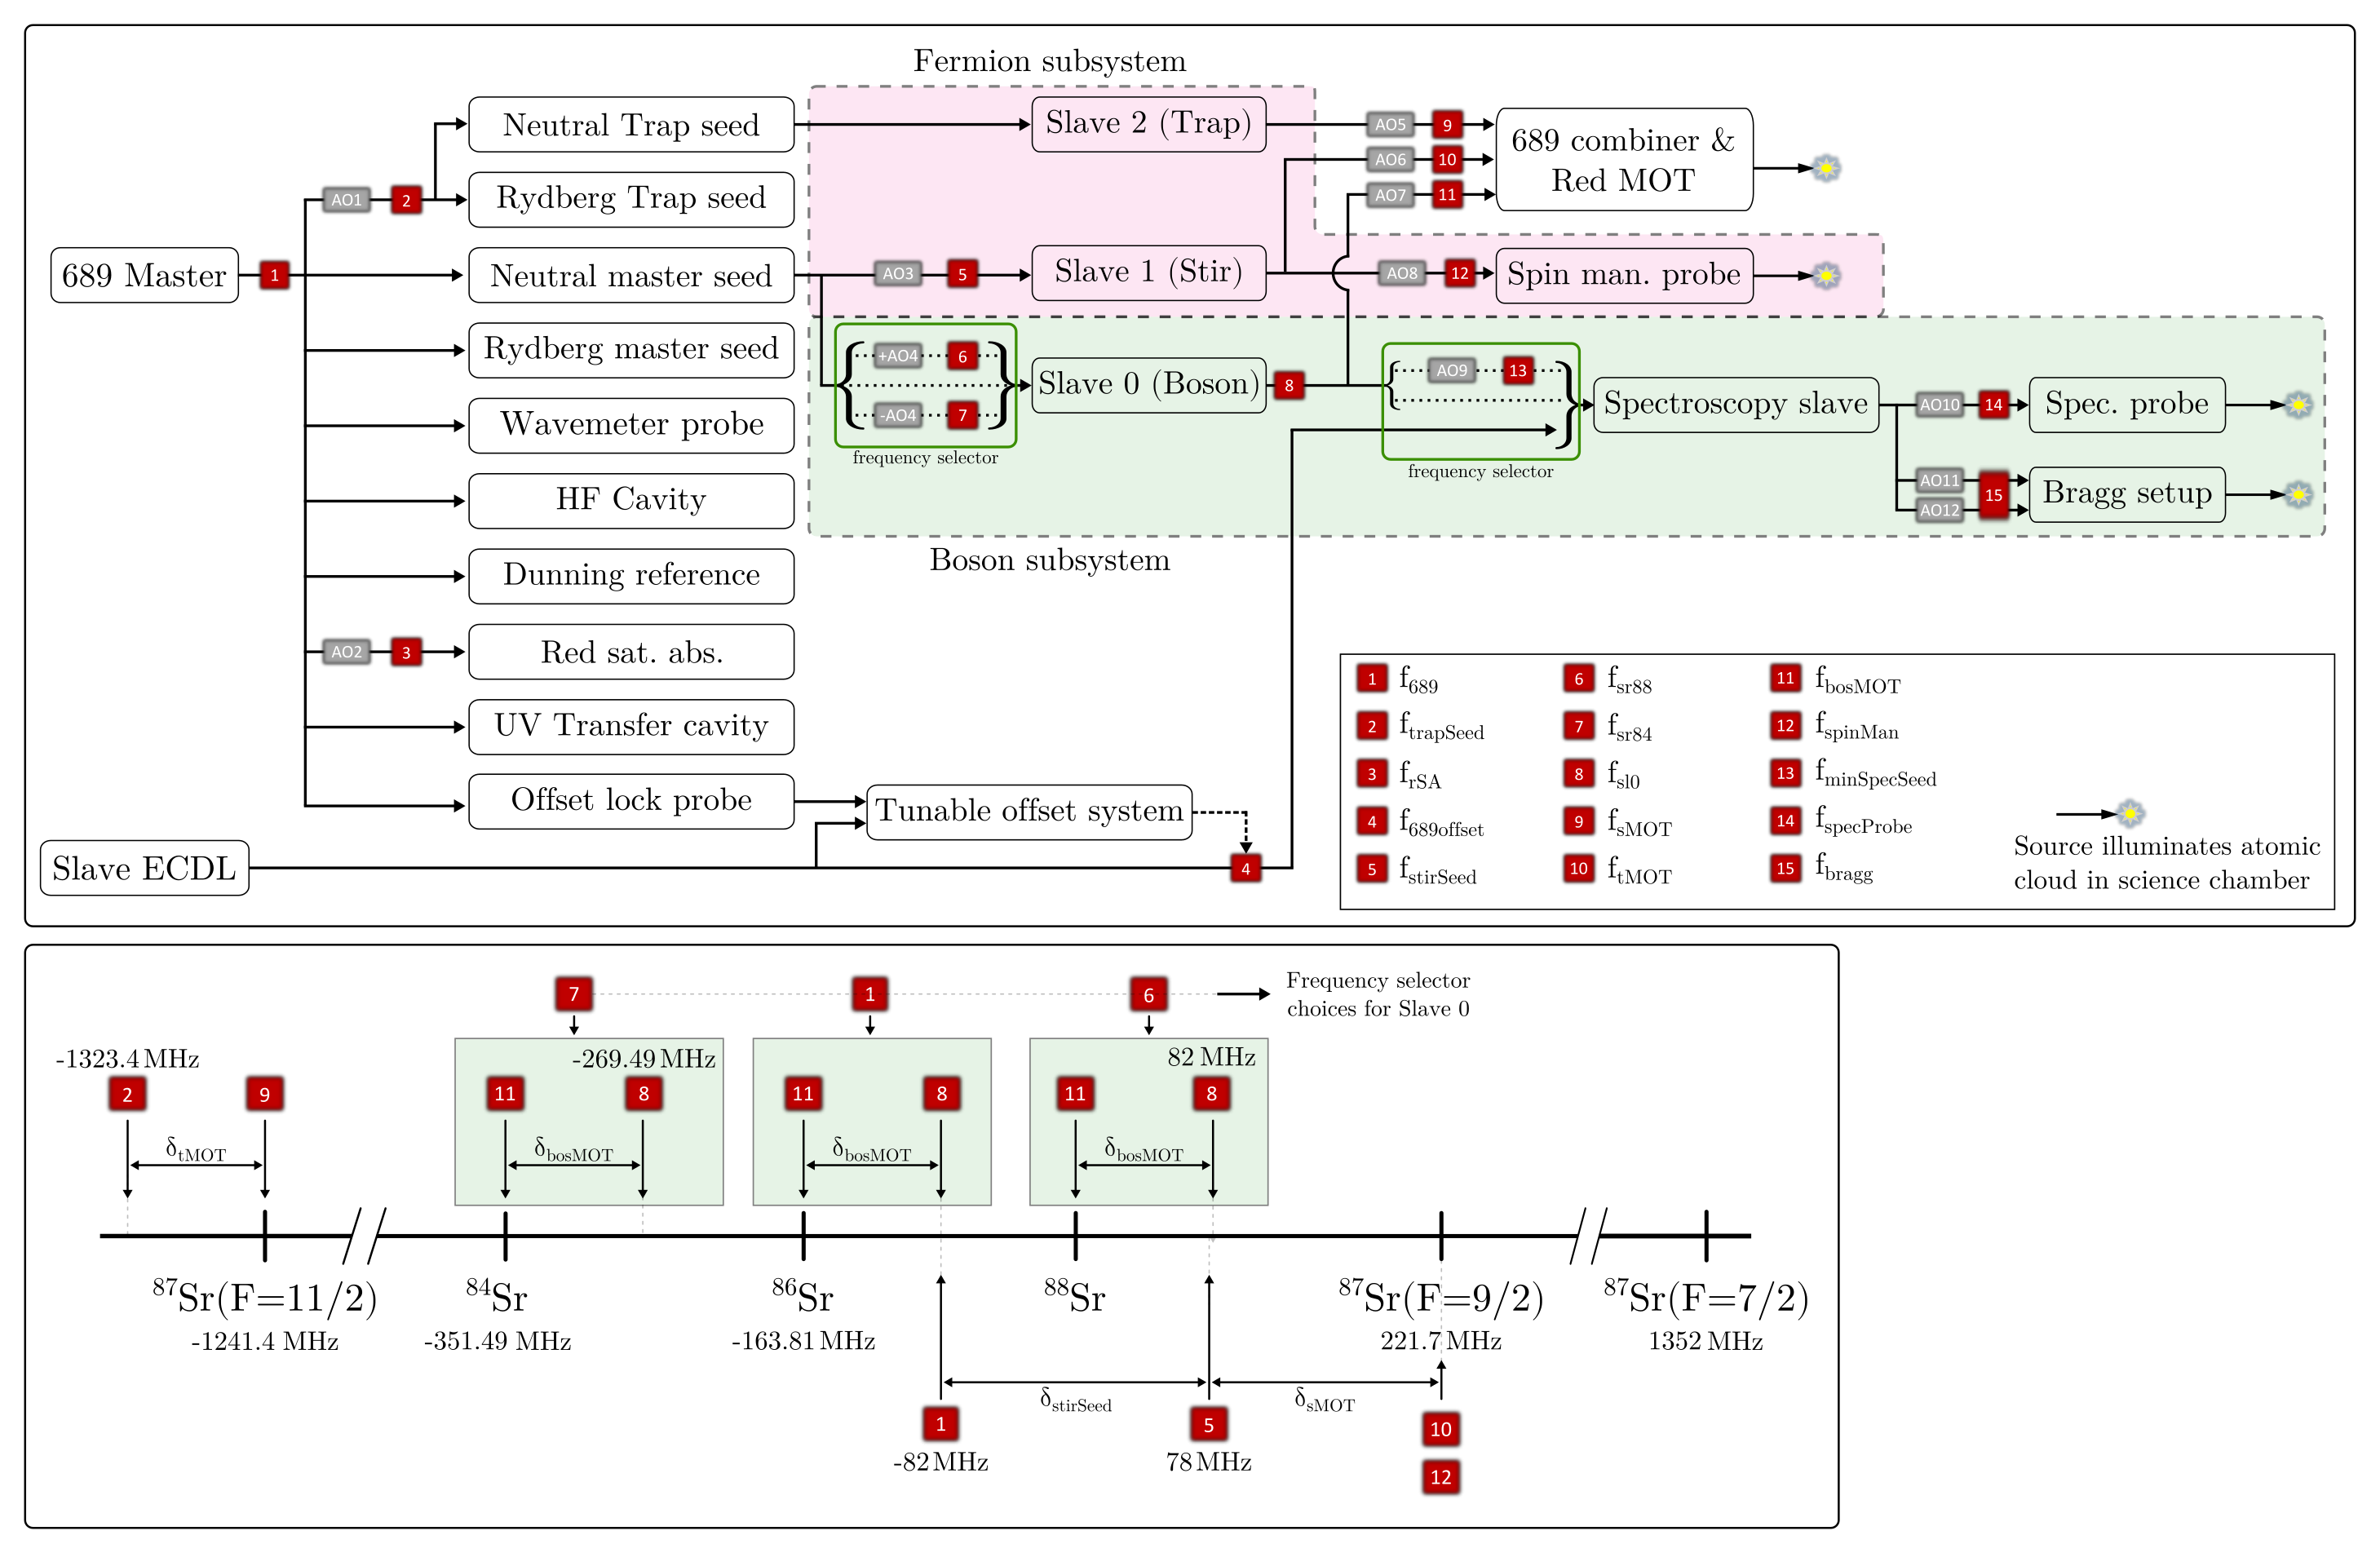
\includegraphics[width=1.3\textwidth,angle=90,origin=c]{689_redSystem.png}}
		\caption{689\,nm light generation system}{Top - Block diagram showing the relations of the various systems, AOMs, and frequencies in use throughout the red system. See Table \ref{tab:689AOM} for information on the AOMs. Bottom - Relevant frequencies for trapping using the Neutral red system.}
		\label{fig:689blockSys}
	\end{figure} 
In conjunction with the block diagram, Table\,\ref{tab:689AOM} details the frequency shifts and AOMs. 
The block diagram denotes the position of these AOMs by the grey squares and the red squares define the various system frequencies determined by the various shifts.
\begin{table}[]
\centerline{
\resizebox{0.8\textwidth}{!}{%
\begin{tabular}{@{}|l|c|c|c|l|l|@{}}
\toprule
\multicolumn{1}{|c|}{\textbf{Label}} & \textbf{Ind.} & \textbf{\begin{tabular}[c]{@{}c@{}}Shift\\ variable\end{tabular}} & \textbf{\begin{tabular}[c]{@{}c@{}}Nominal \\ Freq. {[}MHz{]}\end{tabular}} & \multicolumn{1}{c|}{\textbf{Freq. Source}} & \multicolumn{1}{c|}{\textbf{AOM Model}} \\ \midrule
Trap Seed & AO1 & $\delta_{trapSeed}$ & -1241.44 & Novasource G6 & \begin{tabular}[c]{@{}l@{}}Brimrose\\ TEF-1300-200-550\end{tabular} \\ \midrule
Red Sat. Abs. & AO2 & $\delta_{rSA}$ & +164$\pm$0.5 & \begin{tabular}[c]{@{}l@{}}Novatech 409B\\ (Dithered)\end{tabular} & \begin{tabular}[c]{@{}l@{}}IntraAction \\ ATM-1643DA1\end{tabular} \\ \midrule
Stir Seed & AO3 & $\delta_{stirSeed}$ & +160 & Novatech 409B & \begin{tabular}[c]{@{}l@{}}IntraAction \\ ATM-1602DA1\end{tabular} \\ \midrule
\begin{tabular}[c]{@{}l@{}}Isotope\\ Selector\end{tabular} & AO4 & $\delta_{isoSel}$ & \begin{tabular}[c]{@{}c@{}}+164 or\\ -187.49\end{tabular} & Novatech 409B & \begin{tabular}[c]{@{}l@{}}IntraAction \\ ATM-2001A2\end{tabular} \\ \midrule
Trap MOT & AO5 & $\delta_{tMOT}$ & +82 & \begin{tabular}[c]{@{}l@{}}Trap VCO / \\ Novatech 409B\end{tabular} & \begin{tabular}[c]{@{}l@{}}IntraAction \\ ATM-852DA2\end{tabular} \\ \midrule
Stir MOT & AO6 & $\delta_{sMOT}$ & +143.7 & \begin{tabular}[c]{@{}l@{}}Stir VCO / \\ Novatech 409B\end{tabular} & \begin{tabular}[c]{@{}l@{}}IntraAction\\ ATM-1402DA1\end{tabular} \\ \midrule
Boson MOT & AO7 & $\delta_{bosMOT}$ & -82 & \begin{tabular}[c]{@{}l@{}}Boson VCO / \\ Novatech 409B\end{tabular} & \begin{tabular}[c]{@{}l@{}}Isomet\\ 1205C-2\end{tabular} \\ \midrule
\begin{tabular}[c]{@{}l@{}}Spin man.\\ probe\end{tabular} & AO8 & $\delta_{spinProbe}$ & -144$\pm$2 & Novatech 409B & \begin{tabular}[c]{@{}l@{}}IntraAction\\ ATM-1402DA1\end{tabular} \\ \midrule
\begin{tabular}[c]{@{}l@{}}Spec. slave\\ seed\end{tabular} & AO9 & $\delta_{specSeed}$ & -40 & Novatech 409B & \begin{tabular}[c]{@{}l@{}}IntraAction\\ AOM-402A1\end{tabular} \\ \midrule
Spec. probe & AO10 & $\delta_{specProbe}$ & -82$\pm$20 & Novatech 409B & \begin{tabular}[c]{@{}l@{}}IntraAction\\ ATM-902DA1\end{tabular} \\ \midrule
Bragg \#1 & AO11 & $\delta_{bragg1}$ & \multirow{2}{*}{90$\pm$20} & Novatech 409B & \begin{tabular}[c]{@{}l@{}}Crystal Tech.\\ 3110-125\end{tabular} \\ \cmidrule(r){1-3} \cmidrule(l){5-6} 
Bragg \#2 & AO12 & $\delta_{bragg2}$ &  & Novatech 409B & \begin{tabular}[c]{@{}l@{}}Crystal Tech.\\ 3110-125\end{tabular} \\ \bottomrule
\end{tabular}%
}}
\caption{689\,nm systen AOM details}{Ind. labels the AOMs as shown in Fig.\,\ref{fig:689blockSys}. The sign of the nominal freq. indicates the AOM order.}
\label{tab:689AOM}
\end{table}

All precision frequencies of the 689 system are derived from digital synthesizers with mHz accuracy.
The one exception to this is during the broadband red MOT operation when we use voltage controlled oscillators to effectively broaden the laser linewidth.

The boson and fermion sub-systems allow us to simultaneously trap and cool mixtures of a single bosonic isotope and the fermionic 87.
The isotope selector AOM determines which bosonic isotope this system can trap.
Changing between bosonic isotpes requires the shift from the isotope selector AOM to be changed and light recoupled into the injection lock fiber that is aligned to slave 0.

%Notably, the AC stark shift due to the IR laser is strong enough to require optimization of the red MOT parameters in the presence of the light.
%The optimization is complicated by the influence of gravity on the red MOT which causes the single frequency stage to "sag" which must be overlapped wit the IR light in order to load most efficiently.
	
Recently, the Neutral 689\,nm system has seen significantly growth and been entirely restructured. 
For notes on the original setup refer to App A.3 \& A.4 in Natali's thesis.
The most notable changes have been the replacement of the homemade master ECDL and the move to fiber based injection locks for all slave lasers on the Neutral table.
Furthermore, the master laser system is now shared between the Rydberg and Neutral laboratories and therefore a more modular approach was adopted to ensure independence of the labs experimental schedules. 
This process began with the replacement of our homemade Littman-Metcalf ECDL 689 master with a Toptica DL-Pro system. At the time of this writing (spring 2019) we are currently in the process of migrating from the original high-finesse cavity used for the last 15 years \cite{Nagel2004} of the experiment to an ultra-low expansion cavity system. 

This approach to sharing the 689 light is based on fixing the lock point of the 689 light and fiber coupling this fixed frequency light to the separate experiments. 
From this master fiber we utilize a series of AOMs to choose the correct frequency needed for the experiment at hand. This movement to a fiber based system culminated in the spring of 2018 when the Neutral apparatus significantly refactored our red system and transitioned to an entirely fiber based injection locking scheme. 
Optical fibers provide several key advantages when used to injection lock slaves, namely a much cleaner TEM00 output mode that can be easily mode-matched to the slave. 
Additionally, fibers provide a quick and effective means for ensuring optimal alignment of the injection locking light by coupling the rejected light from the slave diode "backwards" through the fiber. 
Although rejected light is typically minimized when setting up a slave diode, by temporarily placing a waveplate before the isolator you can scramble the input polarization and increase the rejected power to facilitate alignment through the fiber. 
This process generally results in a quite robust alignment of the fiber output and the laser diode and is much faster than the free space method of coupling over a long distance. 
This alignment advantage along with improved mode matching has allowed us to injection lock a slave diode with as little as 300 $\mu$W while producing up to 24 mW of usable output power.

The rest of this section will detail the setup of the 689 system including the master system and both boson and fermion subsystems used for narrowline cooling and trapping.
The primary spectroscopy system and spin polarization setup are outlined in section \hl{ref}.
	
\subsubsection{689\,nm Master}

Optical schematic
	\begin{figure} 
		\centerline{
		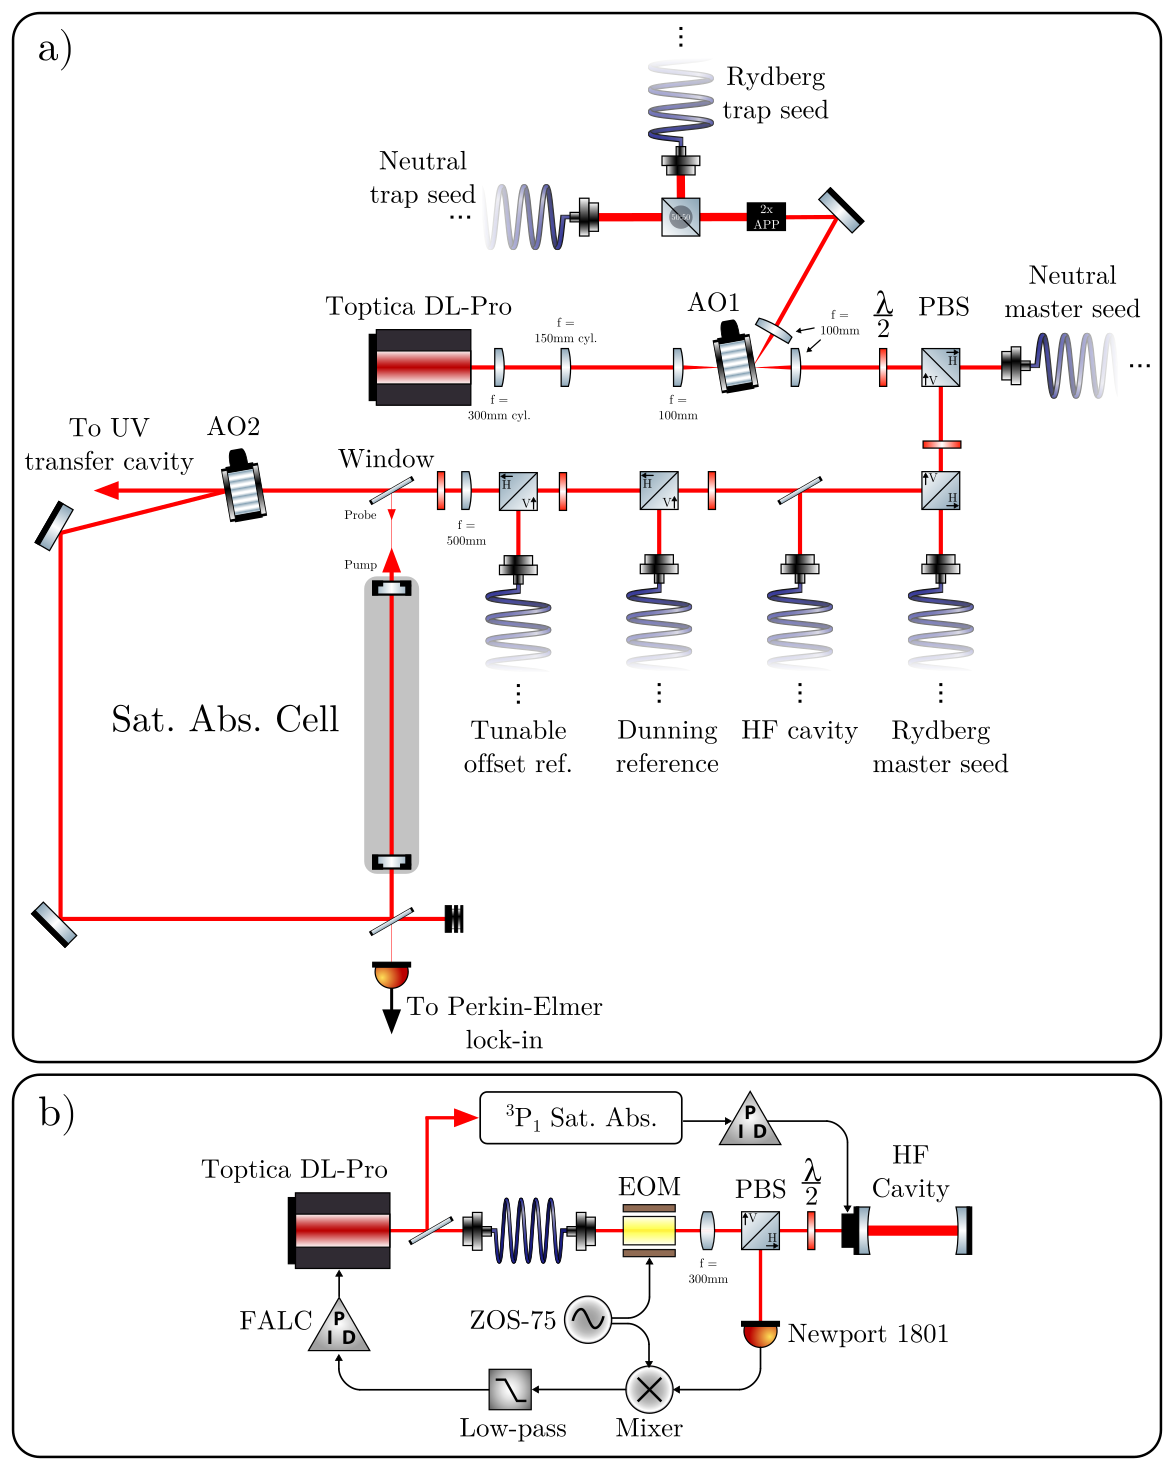
\includegraphics[width=\textwidth]{689_master.png}}
		\caption{689\,nm master optical setup}{The 689 master laser sees }
		\label{fig:689master}
	\end{figure}

%Description
%	Original reference
%Diagram
%Components
%	Mounts
%		Riser
%	Optics
%		Fiber mounts and launchers
%	Circuits
%		FALC connections
%		RF setup
%	Systems
%		High finesse cavity
%		Sat. Abs. 
%		Gigahertz AOM
%Typical running characteristics
%	DLC-Pro settings
%	FALC settings
%		Figures of linewidth
%		measurements of noise
%Profiles
%Tips for operation
%History
%
%
%Locking diagram

\paragraph{High finesse cavity}
The narrow linewidth of the intercombination transition makes it attractive for use in a slew of applications since it is trivial to detuning by thousands of linewidths using conventional acouto-optic modulators.
The conventional method to narrowing the linewidth of a laser is to use an extremely narrow linewidth optical cavity as a frequency discriminator.
Such high finesse (HF) cavities are common place in atomic physics experiments and practically required for any strontium experiments.

Locking diagram
The frequency is sabilized using by deriving an error signal from a saturated absorption cell.
	\begin{figure} 
		\centerline{
		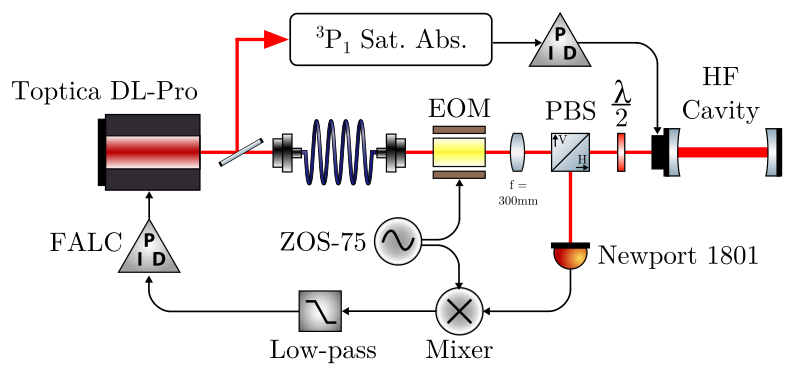
\includegraphics[width=0.6\textwidth]{689_StabilizationSchematic.png}}
		\caption{689\,nm master frequency stabilization}
		\label{fig:689freqLock}
	\end{figure}
	
	

\paragraph{689 sat. abs}
Optical shcematic
How much power?
We typically run at 400 \degree.
The frequency modulation is derived from the fast switching of the RF driving the sat. abs offset AOM.
The frequency

The remaining power from the master system outlined above is sent to a long heat pipe in order to interrogate the intercombination transition.
The error signal is generated using standard frequency modulated Doppler free saturated absorption as is done for the 461 system.
Fig something outlines the optical schematic for this system.
A maor difference compared to the 461 sat abs is the absence of a second pump(probe?) beam that is used to subtract off the Doppler broadened profile.
The red system is able to acheive this since the Doppler broadened profile is approx. 1 GHz compared to the natural line width of 7.5 kHz so any curvature due to the Doppler profile is not significant over the narrow linewidth.
In practice, it is difficult to acheive the transitions natural linewidth through this setup as a number of broadening mechanisms can dominate such as time-of-flights broadening and power broadening.
We find that our Lamb dip has a linewidth of approx. 300 kHz
We have attempted several improvements to narrow width but observe our Lamb dip to have a linewidth 


\paragraph{Measuring the laser linewidth}
Several important factors have seemed to conspire to limit the acheivable linewidth of the Toptica DL-Pro.
While we have pursued improvemenets to the laser system and attempted to maximize the locking badnwidth through short cables and commercial fast analog locking electronics, we find that the laser linewidth is limited to approx. 30 kHz.
Whereas similar implementations in various laboratories have reported laser linewidths of 1 kHz as readily achevieable \hl{refs??}.

Currently we attribute this large width to two main sources. 
First, the high finesse cavity is a homemade system and as reported in App. A.6 of Natali's thesis, has a linewidth of 200 kHz. 
Second, the cavity length is stabilized via interrogating the transition in a sat abs and where the locking signal linewidth is approx. 300 kHz.
Currently, a new ultra-low-expansion cavity is being tested and characterized to replace the homemade HF cavity which we hope will lead to a significant improvement in the laser linewdith.

The expected linewidth of the laser is quoted from Toptica to be on the order of 10 kHz.
However, this measurement is done using \hl{name of technique}, which requires extremely long optical fibers (on the order of 1 km) so it is not currently feasible to verify their claimed linewidth.
As we do not have the correct tools to measure the laser linewidth directly, we must rely on indirect measurements of atomic spectroscopy.
We performed two measurements through measuring the timescale for loss of coherence during a Rabi oscillation and confirmed through direct atom loss spectroscopy.
Fig something shows an example Rabi oscillation and the convergence of the decoherence rate as the lasr intensity is reduced.
While there are many sources that can contribute to the loss of atomic coherence, the dependence on laser power is suggestive.
Additionally, Fig something shows an example of atom loss spectroscopy at extremely low laser intensity.
The measured linewidth of this loss feature agrees with the 30 kHz obtained from the Rabi oscillation measurements.

COnvergence of timescale to a fixed linewidth?

\subsection{Neutral red system}
	\begin{figure} 
		\centerline{
		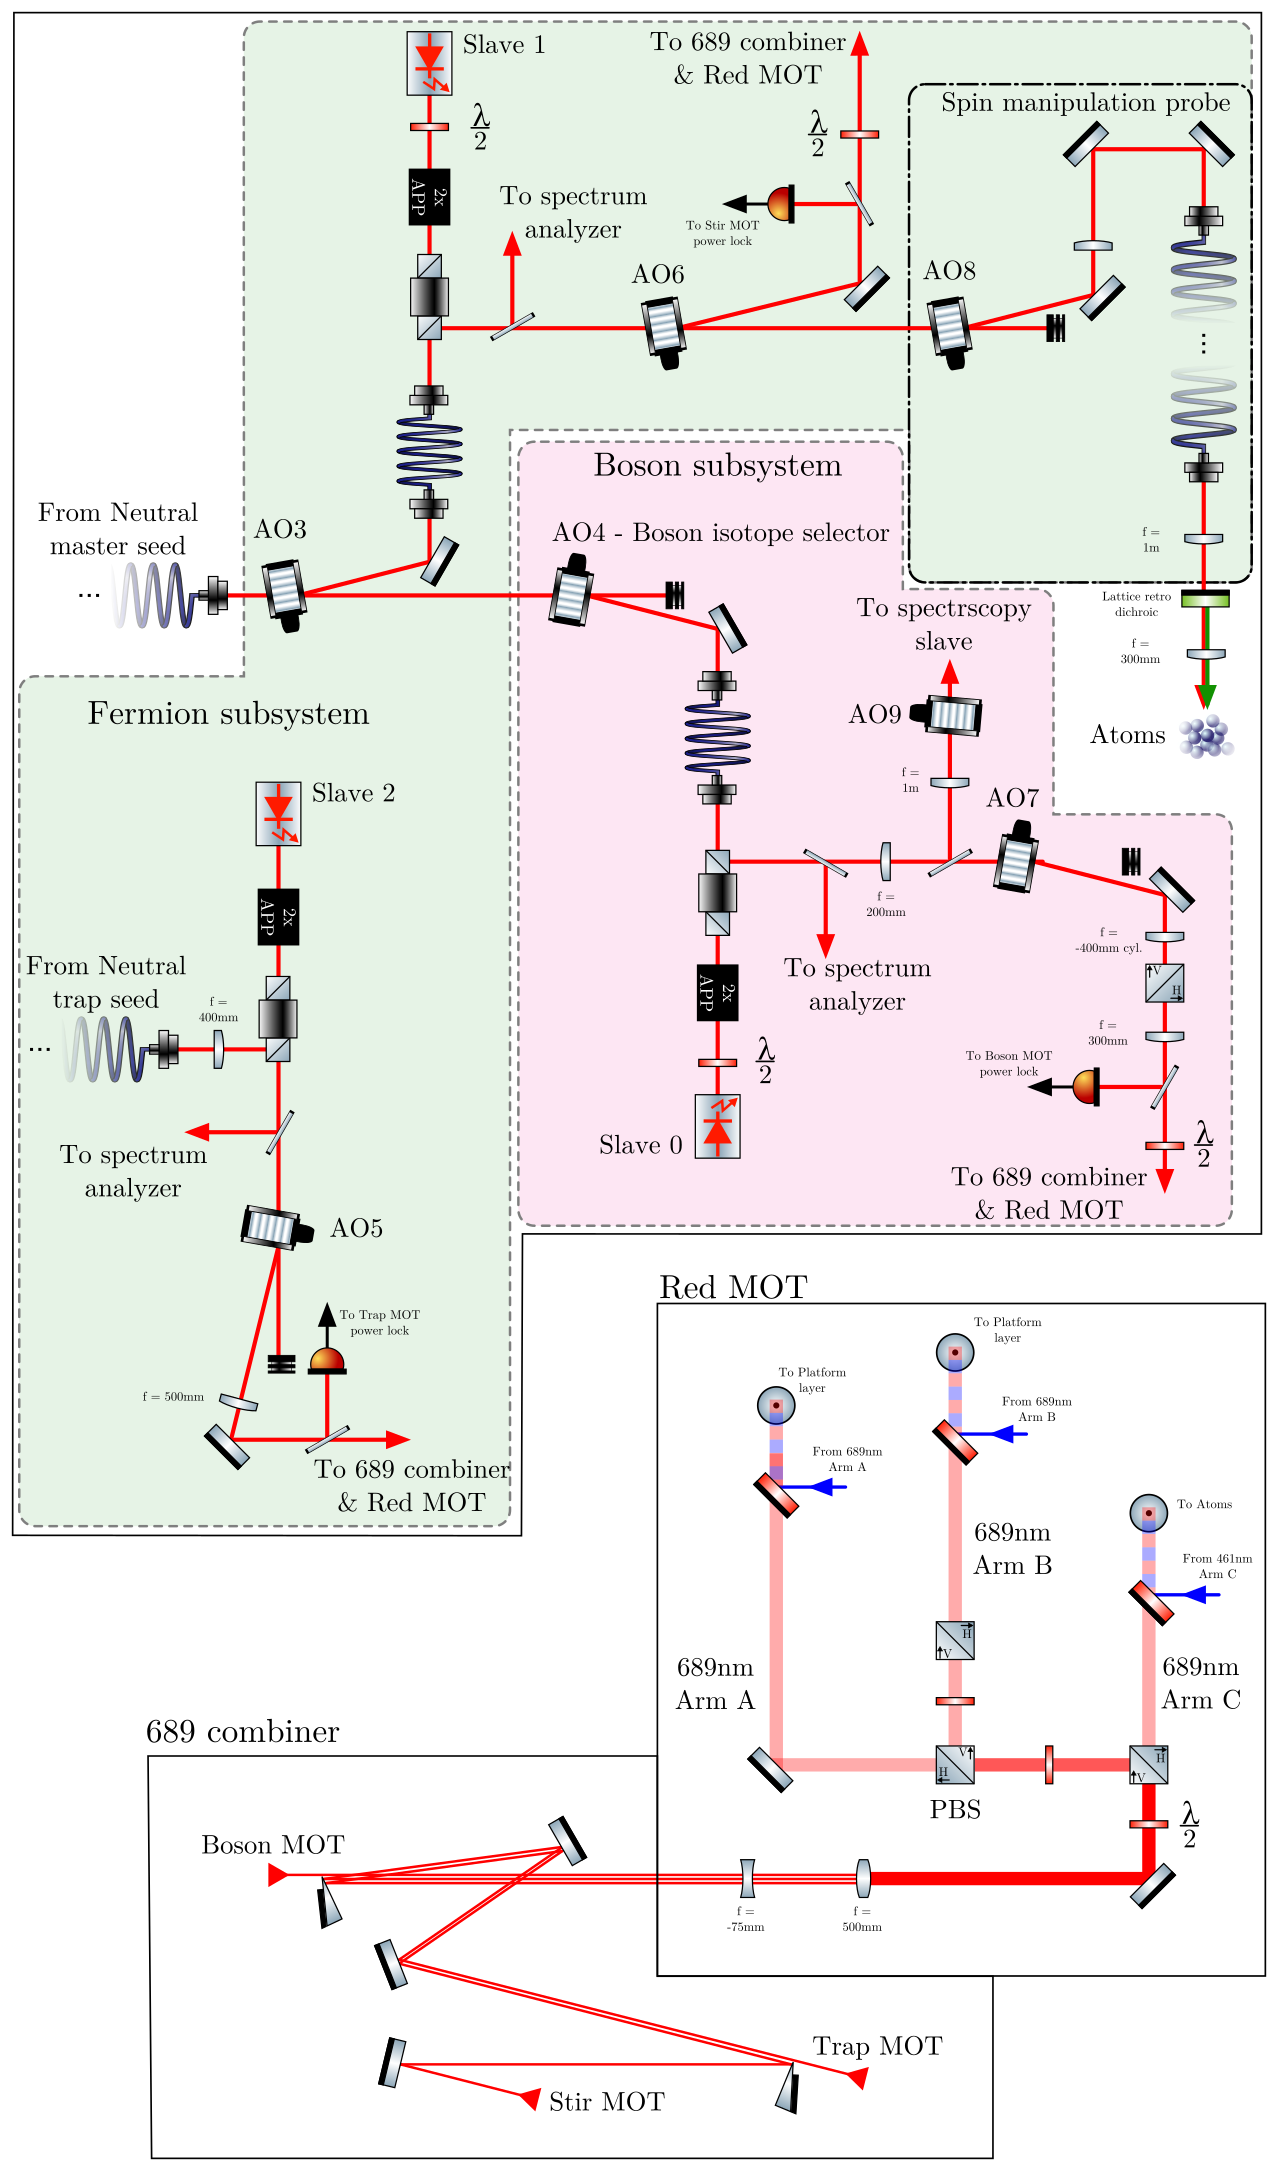
\includegraphics[height=\textheight]{689_neutralRedSystem.png}}
		\caption{Neutral 689\,nm trapping and cooling setup}{}
		\label{fig:neutralRed}
	\end{figure}
	
Light from the 689 master is directed to the Neutral experiment via a fiber connection.
From this approximately 3.3\,mW available at this output, we pass through two AOM's placed sequentially before separating out the requisite beams and directing them to the slave diodes for injection locking.

\subparagraph{Boson subsystem}
Fairly simple system with a slightly complicated method for switching between various bosonic isotopes.

Optical schematic and components
The boso

The 689 combiner + MOT path outlined in the figure is elaborated in figure.
This component is for overlapping the various laser beams which for the bosonic MOT, the fermionic trap and stir MOTs.

In order to change isotopes the aom of the boson selector must be changed according to something.
When swtiching between 88 and 84 this requires that the OMm be flipped around.
We have tested the reproducibility of this scheme and found it to be a simple of effective means for switching between various isotopes.
The MOT aom is run at a constant -82 MHz, therefore the three frequncies for choosing between the various isotopes are to land the input light to the blue of the the atomic trantion by 82 MHz.

Single mode oeration is monitored using spectrum analyzers 



%Description
%Diagram
%	Profiles?
%Components
%	optics
%		isolator
%		cubes
%		lensess
%	mounts
%		custom diode holder
%	aoms
%		RF circuits
%	circuits
%		temp controller
%		current controller
%	Spectrum analyzer
%		reference?
%		refer to the better version developed by Roger
%Runnign characteristics
%	Example spectrum?
%	MOT path powers

\subparagraph{Fermion subsystem}
Discuss the combination of all the paths using the D mirros and how you have to try and do the best you can with alignment. Typically found it best to align beams to center on the cubes and align to the chamber picking one of the paths. Then when adding additional path be careful to only touch the last two mirrors which independetly affect that path.


Description
Diagram
	Profiles?
Components
	optics
		isolator
		cubes
		lenses
	mounts
		custom diode holder
	aoms
		RF circuits
	circuits
		temp controller
		current controller
	Spectrum analyzer
Runnign characteristics
	Example spectrum?
	MOT path powers


Description
Diagram
	Profiles?
Components
	optics
		isolator
		cubes
		lenses
	mounts
		custom diode holder
	aoms
		RF circuits
	circuits
		temp controller
		current controller
	Spectrum analyzer
Runnign characteristics
	Example spectrum?
	MOT path powers
	
\subparagraph{689 combiner \& MOT}
Optical schematic of the combiner showing how the beams skirt by one another.
Long path lengths ensure fairly good co-propagation but it is not perfect.

The 689 combiner is a series of cloesly aligned mirrors for combining the boson, stir, and trap MOT beams before sending into the red MOT path and ultimately to the atoms.
Another popular way this is acheived is via fiber coupling but this is a lossy process.
Not perfectly aligned but it is good enough.

Give schematic
\pagebreak


\subsection{Optical dipole trap: 1064\,nm} \label{ssec:1064sys}
The 1064\,nm optical dipole trap is our primary science trap.
Since strontium has a J=0 ground state, magnetic traps that are common to alkali's cannot be used for trapping the strontium ground state.

There are two paths split, named the loading arm and the sheet/dimple arm as shown in Fig.\,\hl{some fig}.
Several diffferent types of traps have been formed, ref Ying thesis. 

How much power roughly is split between the arms?

AOMs are back to back which couples the power stability of the two arms. 
This setup allows us to more fully utilize the available power from the IPG and in practice while two completely decoupled independent arms may add a slight complication, when accounted for this has generally not been a major source of concern. 
Although, we have found it useful to continuously monitor the evaporation trajectory from shot to shot. 
As a problem, say with a misbehaving power lock, along one arm are is now coupled and may result in intensity fluctuations along both arms if the power lock cannot account for this perturbation.

Give stats on the loading path The loading path has the ability to be recycled on itself but we have not utilized this capability in many years due to complications of measuring the trap frequencies. 

The sheet/dimple arm can take two configurations as it's name implies. The sheet trap is an approx. 400 x 40um sheet with the short axis parallel along gravity. This geometry is useful for the low densities needed for Sr 86 to minimize the effecs of three body recombination. Alternatively, by switching out a mirror we can direct this power 

evaporation and description of density distribution
Formula for ramp
ref for where we get the formula and what it's purpose is

\subparagraph{Historical note:}
In the fall of 2018, the IPG YLRsomething, which had been in use for about a decade, died due to a thermal issue which led the internal fiber amplifier to overheat and burn.
As of April 2019, this laser is being replaced by \hl{something} and Josh Hill is reconstructing some elements of the paths reported here and in Ying's thesis.
Therefore, as his forthcoming thesis will outline this work in detail, we will focus our discussions on the general usage and procedures of the 1064\,nm trap.


\paragraph{Alignment Procedure} \label{sssec:1064_align}
Will focus on independent arm alignment of loading trap and sheet trap
Also useful to imagine three orthogonal axes with their origin set at the center of the chamber.
Fig.\,\hl{something} shows the propagation of the IR beams with respect to the science chamber


%% Loading
From the figure, we see that the loading trap propagates primarily along the X-direction. 
We start by aligning loading trap since it is generally less sensitive and the ports that it goes through are equidistance from the origin

Can generally get away with centering vertically on the chamber windows. 
goal is to rotate about the center point, can verify this by equalizing the distance from the edge of the window on both sides of the chamber
Letting the atoms extend along a single dimension of the trap. 
Moving the red MOT up and down with the z-trim. Dynamic control of z-trim is useful here as you can define a loading b field value then a science b field value.

As a secondary option, there are shortpass dichroic in place with fiber launchers positioned behind htem.
Use the shortpass dichoric mirrors to counter propagate a red loss beam. Alignment of the red beam follows the usual procedure making sure to reduce the exposure time and power as low as possible while maintaining a loss signal which should maximize alignment.


%% Sheet

%%%% Scratch
Best method is to copropagate with 689

The sheet trap propagates primarily along the y-axis. This direction has one port extended away from the main chamber body due to the ion gauge. This can complicate the alignment. You

is a little more complicated because it is very sensitive

For peaking up the the sheet trap alignment, hit the red MOT with the loading trap, then extinguish the red MOT away and hold in the single arm loading trap for approx 10-20ms. 
This allows the red MOT to fall away and the atoms caught in the ODT will expand along the arm, mapping out the spatial profile.
Once the untrapped atoms have fallen away, image the the atoms in situ (i.e. without a time-of-flight). 
With the spatial profile outlined you should be able to scan the sheet trap vertically looking for horizontal confinement along the loading trap. As the sheet is so tight along the vertical direction, this alignment is done using the last cylindrical lens before the chamber. 

Dimple trap follows the same process as the sheet alignment but there is a Newport Pico motor for finely adjusting instead of a lens.


\subsubsection{Trap frequency calibration} \label{sssec:1064_trap_freq}
Measurement of trap frequencies had previously relied upon parametric heating via intensity modulation of the optical dipole trap \hl{cite Ying thesis}. 
This process would observe atom loss via resonant heating when the modulation frequency matched a trap oscillation frequency. 
While this is a convenient and simple process it can lead to quite a complicated spectrum since the heating process does not discriminate directional information and may lead to coupling of higher harmonics of the trap frequencies. 

Recently, we have found excitation of center-of-mass (COM) oscillations to be a more reliable mechanism for measuring trap frequencies.
Fig.\,\hl{something} shows an example of trap frequency measurements taken via center-of-mass oscillations.

Vertical trap frequencies is a straightforward process whereby we can excite oscillations by quickly extinguishing the trap for $\approx$1-2\,ms before turning them back on.
By varying the evolution time once the trap is restored followed by a typical time-of-flight and absorption imaging, then we can observe the oscillations and fit the variation of the cloud center position over time to extract the frequency.
On a technical note, we find that this rapid on-off of the beams results in a brief overshoot of the power locks when turned back on.
However, the power lock equilibrium is restored after a few milliseconds and therefore we evolve for a time long compared to this perturbative behavior.

Exciting oscillations along the horizontal directions, X and Y, is a bit more challenging.
We have developed two mechanisms for exciting these modes which we call the kicking method and the pulling method.
The following sections will provide further detail.

\subparagraph{Kicking method:}
The kicking method has been primarily used for measuring the trap frequencies of the independent arm ODT.
In this configuration the two ODT beams are in plane and orthogonal.
This method is useful in this scenario since the excitation of the center-of-mass oscillation via an abrupt step of the AOM drive frequency.
This changes the deflection angle of the IR beam out of the AOM and "kicks" the cloud.
Briefly, the kicking procedure is 
\begin{outline}[enumerate]
	\1 During the ODT loading phase, load into a trap with one beam offset
		\2 The beam which is offset will excite oscillations along the opposite beam and measure the confinement due to the beam being shifted.
		\2 We have found that, in our current configuration, an offset of $\approx$1\,MHz results in a reasonable excitation amplitude.
	\1 Once the red MOT is extinguished and ODT loading is complete, we evaporate down to the trap of interest in the offset trap.
		\2 Here we find it useful to follow the evaporation trajectory for the experiment at hand. This is done so we can adequately model the potential and evaluate the trap depth.
	\1 After evaporation, we let the atoms equilibrate for $\approx$250\,ms then suddenly switch the frequency of the trap and hold for a variable evolution time before releasing and imaging.
\end{outline}

We achieve the frequency shift that excites the kick by stepping the input of a voltage controlled oscillator (VCO) which is typically fixed by a static voltage source.
During the experimental setup, we account for any voltage offsets between sources by measuring the output frequency of the VCO using an RF meter.
This is also ow we determine the needed voltage change for the $\approx$1\,MHz shift.

\subparagraph{Pulling method:}
With the recent addition of the high power 532\,nm for the optical lattice, we have explored an alternative method of inducing a center-of-mass oscillation. 
This method uses a single pass of vertically propagating green light (Arm C) to pull the atoms out of equilibrium and excite an oscillation.
Details of the setup are are given below in \ref{p:armCFirstPass}.

The pulling method has become our preferred method as it does not require us to change any AOM frequency sources as the kicking method has\footnote{Loading trap uses VCO so changing the voltage source is enough. However, the sheet/dimple is run from a IntraAction driver with a fixed digital synthesizer as the input. For this measurement we temporarily replace the synth with a VCO, but be careful as this will also change the gain of the power lock circuit (Synth outputs $\approx$0\,dbm but VCO outputs $\approx$10\,dbm)}.
Additionally, the pulling method can be applied to traps where the 1064\,nm light is recycled whereas previously our only recourse was te intensity modulation previsouly described.

\subsubsection{Modeling the potential} \label{sssec:1064_modeling}
Optical dipole traps result from the spatial dependence of the AC stark shift present whenever an atom interacts with a light field \cite{Grimm1999a}.
In the simple two-level dressed atom model, the AC stark shift originates from the diagonalization of the atom-photon system which results in an avoided crossing when the photon is nearly resonant with the difference between energy levels \hl{ref on dipole force as avoided crossing, CT book?}
Fig.\,shows a schematic avoided crossing near resonance where the separation between states is defined as $2\Omega$, or twice the Rabi frequency given by
\begin{equation}
	\Omega
	\label{eq:rabiFreq}
\end{equation}
From here we can understand the origin of the potential which provides the trapping force in ODTs.
To see this, consider an atom in the ground state, \ket{1}, and a light field with negative detuning, $\Delta < 0$.
Through the intensity dependence of Eq. \ref{eq:rabiFreq} we see that as intensity is increased the Rabi frequency also increases and correspondingly the energy of the ground state is lowered.
Conversely, when blue detuned, $\Delta>0$, the ground state energy is minimized in regions of low intensity.
The scaling of this change in potential energy is proportional to
\begin{equation} \label{eq:potProp}
	U(r) \varpropto \frac{\Gamma}{\Delta}I(r)
\end{equation}
where, $\Gamma$ is the natural linewidth of the transition determined by it's spontaneous decay lifetime, and $I(r)$ is the spatial dependence of the light intensity.

A subtle question may arise when considering the blue detuned case of Fig.\,\hl{some}.
If the atom seeks to minimize its potential energy, then doesn't the state \ket{2,n=0} represent a lower energy state?
To answer this, we must consider the scattering rate of photons which transition the atomic state from $\ket{1}\,\rightarrow\,\ket{2}$.
This rate is proportional to
\begin{equation} \label{eq:scatRateProp}
	\Gamma(r) \varpropto \left(\frac{\Gamma}{\Delta}\right)^2 I(r)
\end{equation}
Comparing Eqs.\,\ref{eq:potProp} \& \ref{eq:scatRateProp}, we find a favorable scaling for far off-resonant optical traps since the potential energy varies as $1/\Delta$ and the scattering rate varies as $1/\Delta^2$.
Therefore neutral atoms illuminated with high intensity off-resonant light will tend to remain in the ground state while feeling a trapping force, $F(\vec{r}) = -\nabla U(\vec{r})$.

As shown, the spatial dependence of the trapping potential derives from the TEM$_{00}$ gaussian intensity profile of the incident lasers given by.
\begin{equation} \label{eq:gaussInt}
	I(r,z) = \frac{2P}{\pi w(z)^2} \exp{\frac{-2 r^2}{w(x)^2}}
\end{equation}
where $z$ is along the beam propagation axis and $r$ is transverse to this axis.
Additionally, P is the incident laser power, $w_0$ is the waist radius at $z=0$, and the axial profile $w(z)$ is given by
\begin{equation}
	w(z) = w_0 \sqrt{1 + \left( \frac{z \lambda}{\pi w_0^2} \right)^2}
\end{equation}
where $\lambda$ is the laser wavelength.

Combining Eqs.\,\ref{eq:potProp} \& \ref{eq:gaussInt} we find the three dimensional potential generated by two orthogonal lasers to be given by
\begin{equation} \label{eq:indArmPot}
\begin{split}
	U(x,y,z) = m g z + \frac{2\alpha(\lambda)}{\pi} \left[ \frac{P_1}{w_1^y(z)\, w_1^z(z)} \exp{\frac{-2 (y^2+z^2)}{[w_1^y(z)]^2 \,[w_1^z(z)]^2}} \times \right. \\
	\left. \frac{P_2}{w_2^x(z)\, w_2^z(z)} \exp{\frac{-2 (x^2+z^2)}{[w_2^x(z)]^2\,[w_2^z(z)]^2}} \right]
\end{split}
\end{equation}
where $mgz$ accounts for the influence of gravity on the atoms of mass $m$, labels $1,2$ specify the lasers as illustrated in Fig.\,\hl{something}, and $\alpha(\lambda)$ is the AC polarizability of the ground state at a given wavelength.
This polarizability encapsulates the natural linewidth, detuning, and resonant behavior of the light field interaction with the bare atomic states \cite{Grimm1999a}.
Sec. 2.3.1 and App. A of Pascal's PhD thesis \cite{Mickelson2010b} outlines a calculation of the AC polarizability which at 1064\,nm is $\alpha( \lambda = \text{1064\,nm} ) = -10.9$\,Hz/(W/cm$^2$)\,$=-5.23\e{-8}$\,$\mu$K/(W/cm$^2$).
Units here are chosen as convenient lab units and can be converted to SI by $3.52\e{-40}$\,$\frac{\text{J}}{\text{Hz}}$\,(W/cm$^2$))$^{-1}$. 
Furthermore, $w_{(1,2)}^{(x,y,z)}(z)$ accounts for astigmatic laser profiles where the axial propagation along z of the orthogonal beam axes is not described by the same beam parameters.

The effects of gravity are a significant limiting factor for ultracold atoms as it is the dominant force that must be counteracted by the optical dipole trap.
Fig.\,\hl{something} shows the effects of gravity considering a simple one-dimensional gaussian potential, $U(z) = mgz + A\exp{\frac{-2z^2}{\sigma^2}}$.
Here we've chosen a general form of the gaussian for illustrative purposes.
From the figure, we see how to define the trap depth as the difference between the trap minimum and the lowest saddle point.
Furthermore, by making the harmonic approximation, shown by the dashed line, we can Taylor expand Eq.\,\ref{eq:indArmPot} and determine the expected trap frequencies.

From the lower figures we see realistic 3 dimensional profile of our independent arm ODT.
Analyzing the 3D profiles we find that the saddle points may not be along the line $z=0$, therefore we consider the full gradient when searching for the saddle point.
For deep traps (high power) the trap depth is well approximated by teh saddle point along $z=0$.
However, for this configuration at shallow traps (low power) the trap depth is determined to be along a non-trivial trajectory .
This realization has important implications for our analysis of the halo binding energy described in Ch. \ref{ch:chap3}.

\hl{want a 2 part figure. a) 1D plot of mgz+gauss with a harmonic overlaid. b) 3D deep trap. c) 3D shallow trap}

%then by illuminating an atomic sample with intensity light
%
%The separation between states is intensity dependent and using this we see the origin of optical dipole trap.
%
%Fig b shows the case of red tuning, as intensity is increased the separation between stats is increased and thus the ground state energy is overall lowered.
%This results in a varying potential energy surface which produces a force directing the atoms to the region of highest tintensites.
%Conversely, when blue detuned, the energy between states is decreased as the atom moves away from the laser intensity. 
%
% From Pascal
%The simplest dipole trap results from a single laser beam shone onto an atom. 
%A dipole moment is induced in the atom by the electric field of the laser, and the interaction between the laser field and the dipole moment of the atom means the atom experiences a force proportional to the gradient of the Stark shift (“light shift”) of its energy levels:
%Fdipole = -delta(delE) delr
%The gradient is along r which, for the usual Gaussian mode and radial symmetry of a laser beam, is zero at the intensity maximum of the laser and increases as the intensity drops off. 
%The energy levels move either towards or away from each other depending on the sign of the detuning of the light from the resonance frequencies of nearby atomic transitions, thus creating a potential that is proportional to the intensity of the laser:
%Udipole(r) prop Gamma Delta I(r).
%Here, Gamma is the spontaneous decay rate of a transition which is an amount Delta away from the laser frequency.
%Confinement also occurs in the direction of propagation of the optical trap laser if that laser is focused. 
%In that dimension, the maximum of the intensity will be at the waist of the optical trap beam. 
%For a single beam, however, the gradient tends to be much weaker longitudinally than radially, so the atom cloud elongates as the atoms take the shape of the trap. 
%The sign of the detuning plays a role as well (Fig.\,2.15): negatively detuned (red) detuned light moves the ground state energy down, so the trap becomes deeper. 
%But for positively (blue) detuned light, the opposite occurs, creating an anti-trap where atoms are driven away from the intensity maximum. 
%Equation 2.12 is the first of two expressions which encapsulate the key properties of an optical dipole trap. 
%Essentially, it specifies how deep the trapping potential of the optical dipole trap will be for a given laser intensity and frequency. 
%Losses due to scattering are the second important parameter characterizing an
%optical dipole trap. 
%Absorption, and subsequent emission, of light from the trap beam can heat atoms so that they are no longer trapped by the optical potential. 
%The losses due to scattering are also a function of the optical trap laser intensity and detuning,
%For an optical trap laser that is tuned on-resonance with an atomic transition (Delta = 0), both the scattering rate and the trap depth diverge, but the heating rate due to scattering is really limited by the rate that atoms can cycle from the excited state to the ground state. 
%The key difference from Eq. 2.12, however, is that Gammascat approx 1/Delta2, meaning that the rate of heating drops off more quickly with detuning than does the trap depth. 
%As a consequence, trapping neutral atoms in an optical dipole trap is feasible because we can usually find a laser intensity and detuning for which the trap depth is deep enough, but for which the scattering rate is not too high. 
%Finally, it is worth noting that squaring the detuning means that the loss rate is symmetric on each side of resonance, in stark contrast with the asymmetric behavior of Eq. 2.12.
%
%
%Basic theory
%	ac stark shift depends on intensity
%	gaussian beam intensity is spatially dependent
%		Formula for gaussian beam
%	this translates into a spatially dependent potential which can trap
%	must account for gravity
%		1D fig defining trap depth
%Applied
%	With this in mind we can use the above formulas to model the 3D potential from known parameters
%		get the polarizability from previous work by Pascal
%		reference appendix with explanation of program to do this
%	Make the harmonic approximation and solve for expected trap frequencies
%		compare expected and measured, typically get agreement within 10\%.
%	Once we have an accurate model we can find the trap depth
%		3D trap depth is a little more complex then the 1D analysis suggests
%		Fig of one deep 3D potential and one shallow 3D potential
%
%
%
%
%What is Li's different method?
%	he uses builtin jacobian function for finding the gradient matricies 


\pagebreak
\subsection{Optical lattice trap: 532\,nm} \label{ssec:532sys}
Until recently, experiments on the Neutral apparatus were confined to work with bulk gases in an optical dipole trap.
While optical dipole traps are useful for efficient evaporation and thermalization of an ultracold gas, optical lattices greatly extend our capabilites for studying ultracold molecules and novel many-body quantum states \hl{give some refs}.

Optical lattices are formed by a standing wave of light which creates a defect free periodic potential.
These traps are extremely versatile and have enabled the observation of the superfluid - Mott insulator transition \cite{Greiner2002}, artificial gauge fields for neutral atoms \cite{Lin2011}, quantum microscopy with single-site resolution \cite{Bakr2009}, and investigations of quantum magnetism \cite{Hart2015,Greif2015}. 
They are among the most well-established techniques for controlling a quantum state and have proven to be great tools for exploring the connection between few- and many-body systems \cite{Bloch2008}.

\paragraph{Background} \label{sec:latBackground}
An optical lattice is created by counterpropagating two laser beams to form a standing wave pattern, which for two plane waves in one dimension results in a periodic potential given by 
	\begin{equation}
		 V(x) = V_{lat} \; \sin^2(k_L x)
	\end{equation}
where $V_{lat}$ is the lattice depth determined by the polarizability of the atom for a given trapping wavelength $\lambda$ and laser intensity $I$, and $k_L$ is the lattice wavevector.
This potential can be readily extended to three dimensions using two additional pairs of counterpropagating laser beams along the $y$ and $z$ directions which results in a 3D cubic lattice.
Depth of the trapping potential, $V_{lat}$, is controlled by varying the intensity of the lattice beams.

Periodic potentials are powerful because they break the translational invariance of space which results in the formation of band structure and the opening of bandgaps or disallowed particle energies \cite{Ashcroft1976}.
Because of this broken invariance, $p$ is no longer a good quantum number and must be replaced by two new quantum numbers: the band index, $n$, and the quasimomentum, $q$.
In one dimension, quasimomentum is specified by $q = p - nG$, where $G=2\pi/a$ is a reciprocal lattice vector, and $a$ is the real space lattice constant.
Fig.\;\ref{fig:bandStructure} shows how the band structure varies as the lattice depth is increased.
Optical lattices have a lattice spacing $a = \lambda /2$ which determines the reciprocal lattice vector $G = 4\pi / \lambda = 2 \hbar k_L$ and the natural energy scale $E_r = \frac{\hbar^2 k_L^2}{2m}$ where $m$ is the atomic mass and $k_L$ is the lattice wavevector, $k_L = 2\pi / \lambda$.
From the band structure, we see that the bandwidth of each band, given by $\Delta E = E_{q=\hbar k_L} - E_{q=0}$, decreases as the lattice depth is increased.
In the limit that $V_{lat}\!\rightarrow\!\infty$ the band structure reduces to a ladder of harmonic oscillator levels spaced by $\hbar \omega_{ho} = \sqrt{4 V_{lat} E_r}$.
Although, for moderately deep lattices, $V_{lat} \gtrsim 5\,$E$_r$, this approximation is valid near the center of the Brillioun zone, $q = 0$, and provides a simple form to estimate the energy gaps between bands \cite{Jaksch1998,Jaksch2005}.
	\begin{figure} \label{fig:bandStructure}
		\centerline{
		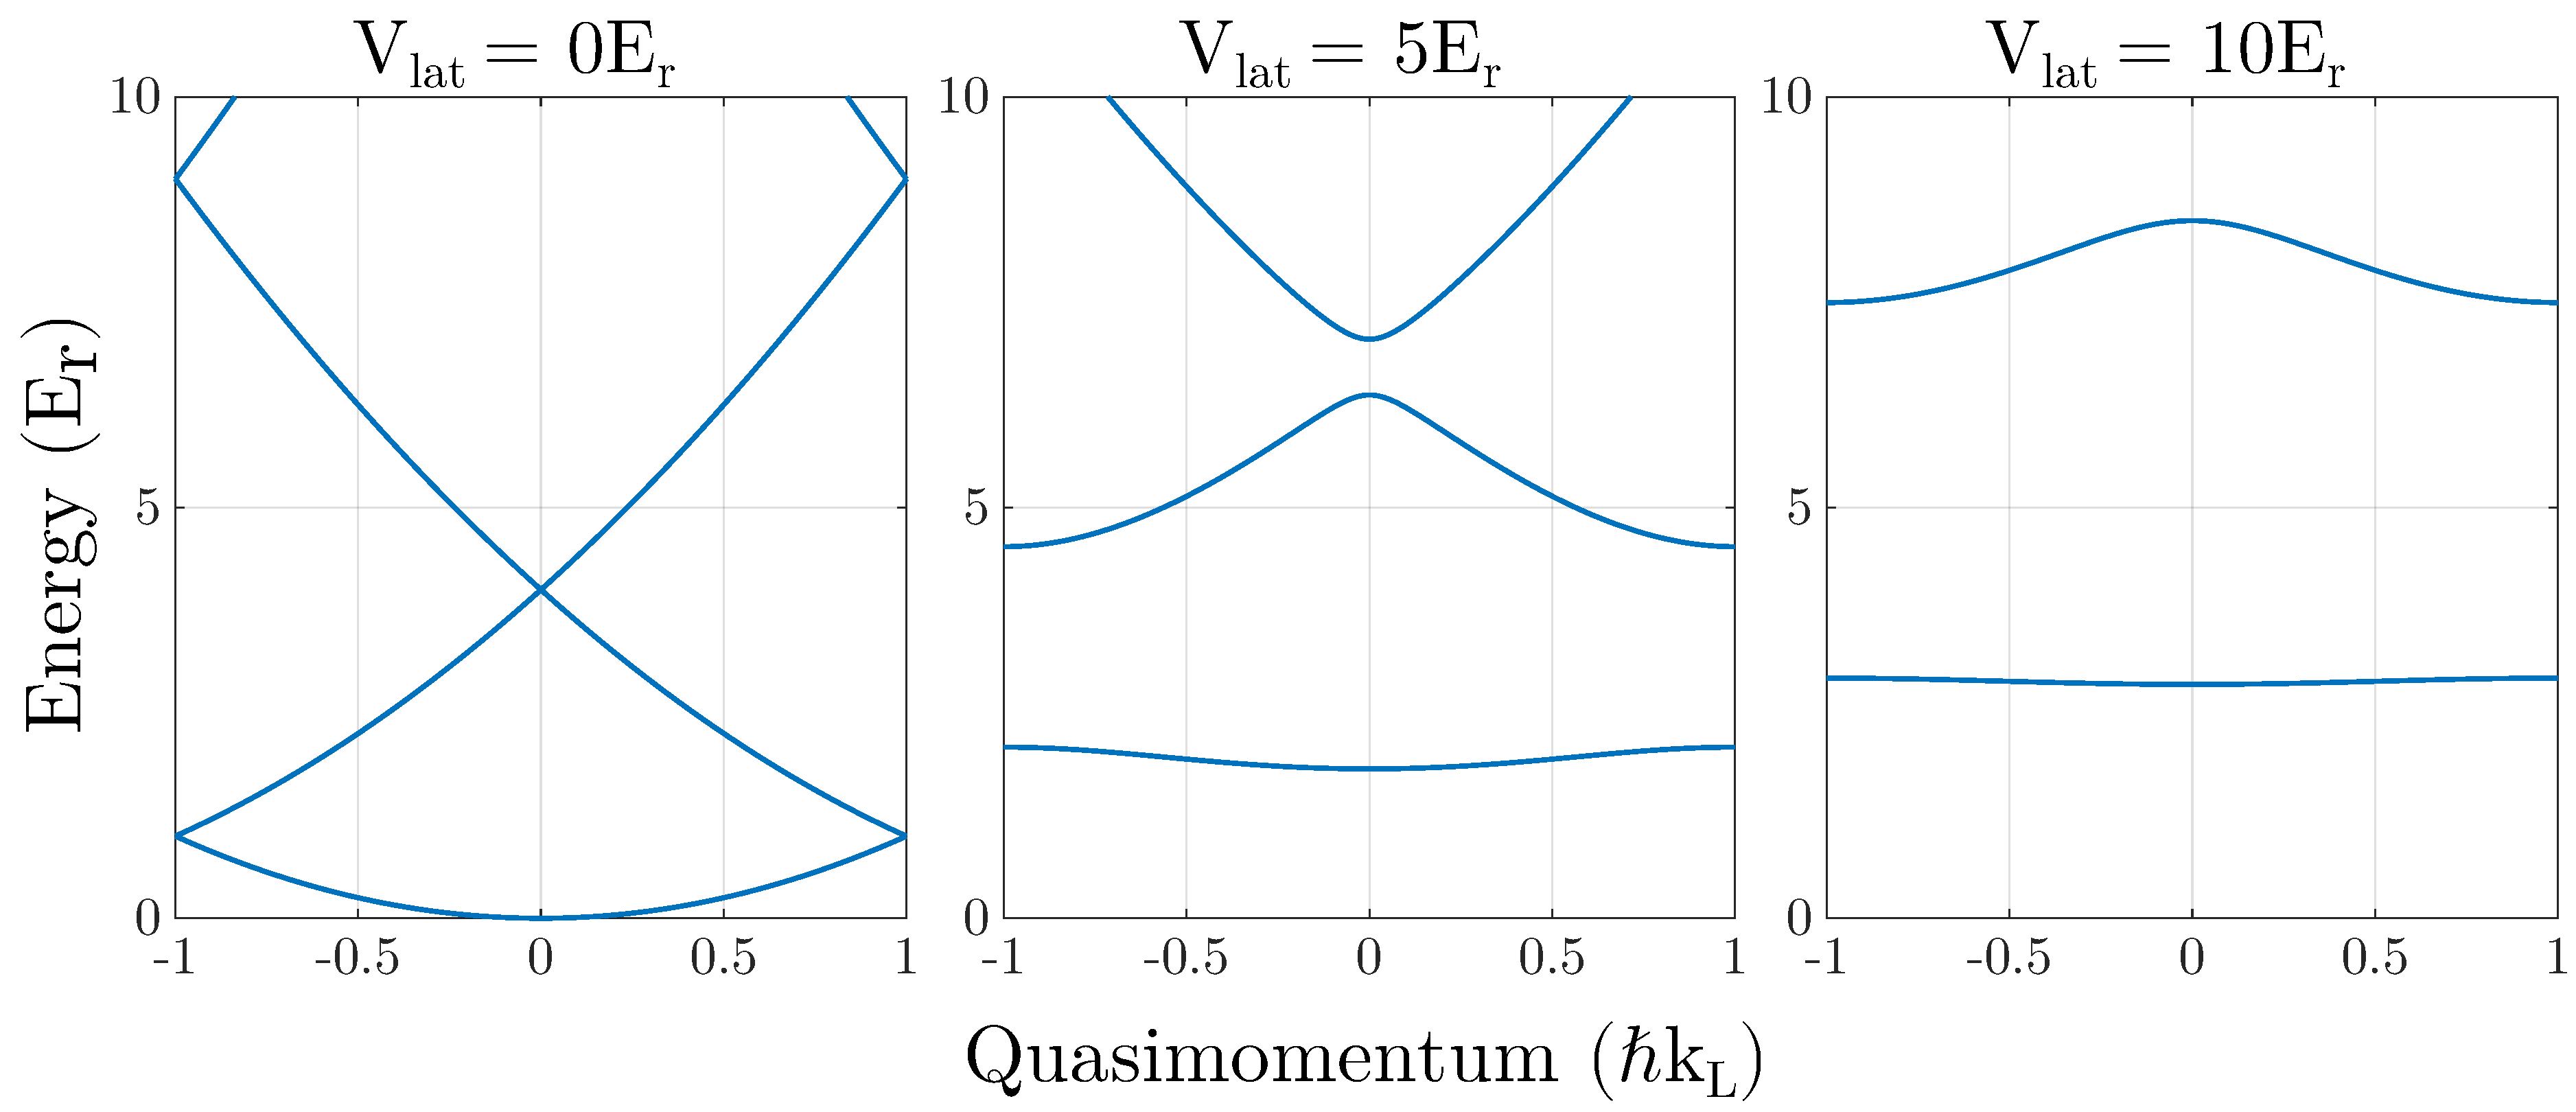
\includegraphics[width=\textwidth]{lattice_bandStructure.pdf}}
		\caption{1D band structure as a function of lattice depth}{One dimensional band structure for an optical lattice as the lattice depth is increased. The band energies are found by solving the Schr\"{o}dinger equation using the Bloch functions of Eq.\;\ref{eq:blochFunc}.}
	\end{figure}
Solutions to the Schr\"{o}dinger equation in a periodic potential are given by the Bloch functions \cite{Ashcroft1976}
	\begin{equation} \label{eq:blochFunc}
		 \phi_q^{(n)}(x) = e^{iqx/ \hbar} \; u_q^{(n)}(x)
	\end{equation}
These eigenstate wavefunctions are specified for a given quasimomentum $q$, and band index $n$. 
Their corresponding energy eigenvalues define the band structure of the lattice shown in Fig.\;\ref{fig:bandStructure}.
From Eq.\;\ref{eq:blochFunc} we see that the Bloch functions are the product of plane waves modulated by a function $u_q^{(n)}(x)$, which shares the periodicity of the underlying lattice potential \cite{Ashcroft1976}.
For an optical lattice this modulating function can be expanded in a basis of plane waves through a Fourier decomposition of the lattice potential in Eq.\;\ref{eq:1dlattice}, which gives \cite{Greiner2003},
	\begin{equation} \label{eq:blochMod}
		 u_q^{(n)}(x) = \sum_l c_l^{(n,q)} \; e^{i2lk_Lx}
	\end{equation}
Here $c_l^{(n,q)}$ are the coefficients for each plane wave in the basis expansion that are found by diagonalizing the lattice Hamiltonian \cite{Greiner2003}.

Often, we are interested in the dynamics of particles on a particular lattice site, but since Bloch functions are delocalized over the entire lattice, it is useful to instead use the Wannier functions. 
These functions provide an orthogonal and normalized set of wavefunctions that are maximally localized to a specific lattice site. 
The Wannier function for a localized particle in the n$^{th}$ band of a lattice site located at position x$_i$ is given by \cite{Jaksch2005}
	\begin{equation} \label{eq:wannier}
		 w_{n}(x - x_i) = \mathcal{N}^{-1/2} \sum_q e^{iqx_i/ \hbar} \; \phi_q^{(n)}(x)
	\end{equation}
where $\mathcal{N}$ is a normalization constant and $\phi_q^{(n)}(x)$ are the Bloch functions of Eq.\;\ref{eq:blochFunc}.
This localized description of particles allows us to calculate important physical quantities which govern dynamical properties of the lattice such as the tunneling rate, $J/ \hbar$, and on-site interaction energy, $U$. 
As $V_{lat}\!\rightarrow\!\infty$, the Wannier functions approach the eigenfunctions of the harmonic oscillator, which allows us to estimate the spatial extent of an atomic wavefunction by $a_{ho} = \sqrt{\frac{\hbar}{m \omega_{ho}}}$ \cite{Jaksch2005}.

\subsubsection{Setup and alignment} \label{sssec:532_align}

\paragraph{Setup}\label{ssec:lattice_setup}

Our optical lattice operates at $\lambda=532\,$nm and is derived from a Coherent Verdi V-18 single mode laser which is sent through separate AOMs for intensity control of each arm before propagating in free space to the atoms. 
We label these arm A, B, \& C as noted in Fig.\,\hl{chamber ref}.
The horizontal arms of the lattice ($x$ and $y$) have $1/e^2$ waists of approx $200\,\mu$m x $200\,\mu$m and their polarization is linear and aligned along the $z$ direction, parallel to gravity. 
The vertically propagating beam has a $1/e^2$ waist size of approx $300\,\mu$m x $300\,\mu$m and polarization aligned orthogonal to the polarization of the horizontal beams. 
With this configuration we estimate we can achieve lattice depths >$30$E$_r$ in an isotropic lattice. 

\begin{table}[]
\centerline{
\resizebox{0.95\textwidth}{!}{%
\begin{tabular}{@{}|c|llr|lr|@{}}
\toprule
 & \multicolumn{1}{c}{Label} & \multicolumn{1}{c}{Part} & \multicolumn{1}{c|}{Position {[}cm{]}} & \multicolumn{2}{c|}{Distances {[}cm{]}} \\ \midrule
\multirow{8}{*}{Arm A} & AOM & IntraAction AFM-804A1 & -126.5 & AOM$\,\rightarrow\,$A1 & 24.1 \\
 & PBS & Thorlabs PBS12-532-HP & -117.8 & A1$\,\rightarrow\,$A2 & 22.3 \\
 & Lens & CVI PLCX-25.4-772.6-UV-532 & -106.5 & A2$\,\rightarrow\,$A3 & 35 \\
 & Dichroic - 1 & Thorlabs HBSY12 & -30.6 & A3$\,\rightarrow\,$A4 & 4.5 \\
 & Dichroic - 2 & Thorlabs HBSY12 & 43.6 & A4$\,\rightarrow\,$AD1 & 10 \\
 & Retro mirror & CVI Y2-1025-0-0.30CC & 69.9 & AD1$\,\rightarrow\,$Atoms & 30.6 \\
 &  &  &  & Atoms$\,\rightarrow\,$AD2 & 43.6 \\
 &  &  &  & AD2$\,\rightarrow\,$ARM & 26.3 \\ \midrule
\multirow{10}{*}{Arm B} & AOM & IntraAction AFM-803A1 & -167.1 & AOM$\,\rightarrow\,$B1 & 19 \\
 & PBS & Newport PBS-5811 & -154.6 & B1$\,\rightarrow\,$B2 & 25 \\
 & Lens & CVI PLCX-25.4-772.6-UV-532 & 103.1 & B2$\,\rightarrow\,$B3 & 46 \\
 & Dichroic - 1 & Thorlabs HBSY12 & -36.1 & B3$\,\rightarrow\,$B4 & 23.5 \\
 & Dichroic - 2 & Thorlabs HBSY12 & 30.5 & B4$\,\rightarrow\,$B5 & 14 \\
 & Retro mirror & CVI Y2-1025-0-0.30CC & 73.5 & B5$\,\rightarrow\,$BD1 & 3.5 \\
 &  &  &  & BD1$\,\rightarrow\,$Atoms & 36.1 \\
 &  &  &  & Atoms$\,\rightarrow\,$BD2 & 30.5 \\
 &  &  &  & BD2$\,\rightarrow\,$B6 & 25 \\
 &  &  &  & B6$\,\rightarrow\,$BRM & 18 \\ \midrule
\multirow{6}{*}{Arm C} & AOM & IntraAction AFM-803A1 & -117.5 & AOM$\,\rightarrow\,$C1 & 45.5 \\
 & PBS & Thorlabs PBS12-532-HP & -109.5 & C1$\,\rightarrow\,$C2 & 25.5 \\
 & Lens-1 & CVI PLCX-25.4-772.6-UV-532 & -89.5 & C2$\,\rightarrow\,$C3 & 15 \\
 & Retro lens & CVI PLCX-25.4-149.9-UV-532 & 14.6 & C3$\,\rightarrow\,$C4 & 5.5 \\
 & Retro mirror & CVI Y2-1025-0 & 18.2 & C4$\,\rightarrow\,$Atoms & 26 \\
 &  &  &  & Atoms$\,\rightarrow\,$CRM & 18.2 \\ \bottomrule
\end{tabular}%
}}
\caption{Lattice optics details}{All measurements are specified in centimeters. The optics position is given with respect to zero defined at the atom position. Distances are referenced to the optics labels given in Fig.\,\ref{fig:532schematic}.}
\label{tab:532sys}
\end{table}

	\begin{figure} 
		\centerline{
		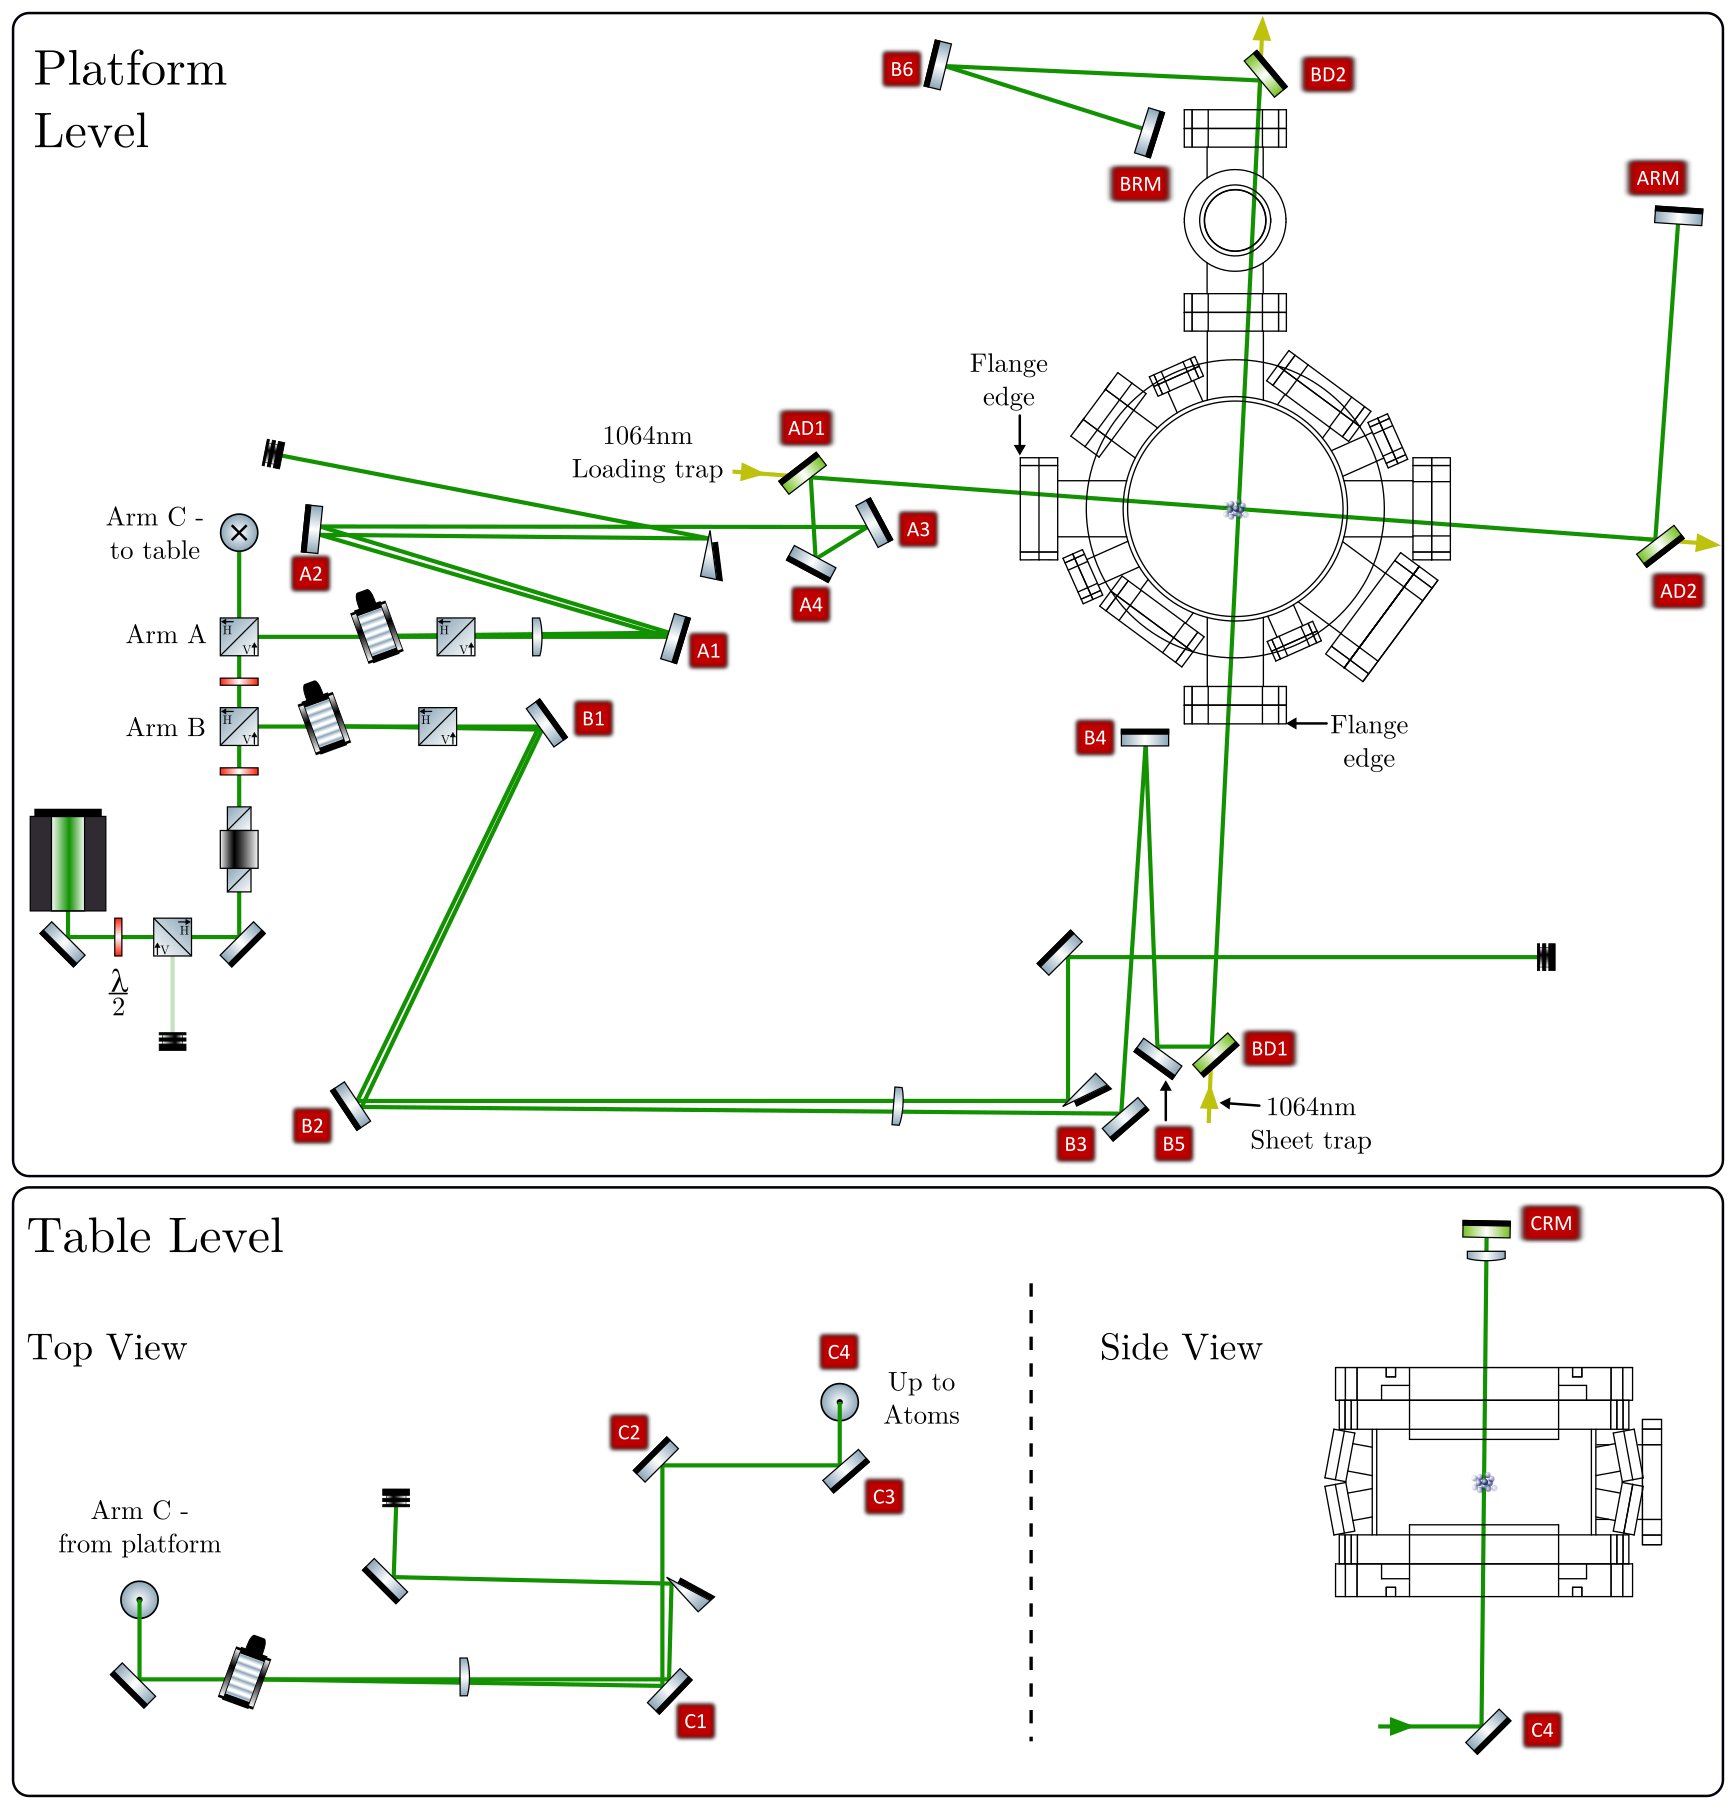
\includegraphics[width=1.2\textwidth]{lattice_schematic.png}}
		\caption{Lattice optical schematic}
		\label{fig:532schematic}
	\end{figure}
	
	\begin{figure} 
		\centerline{
		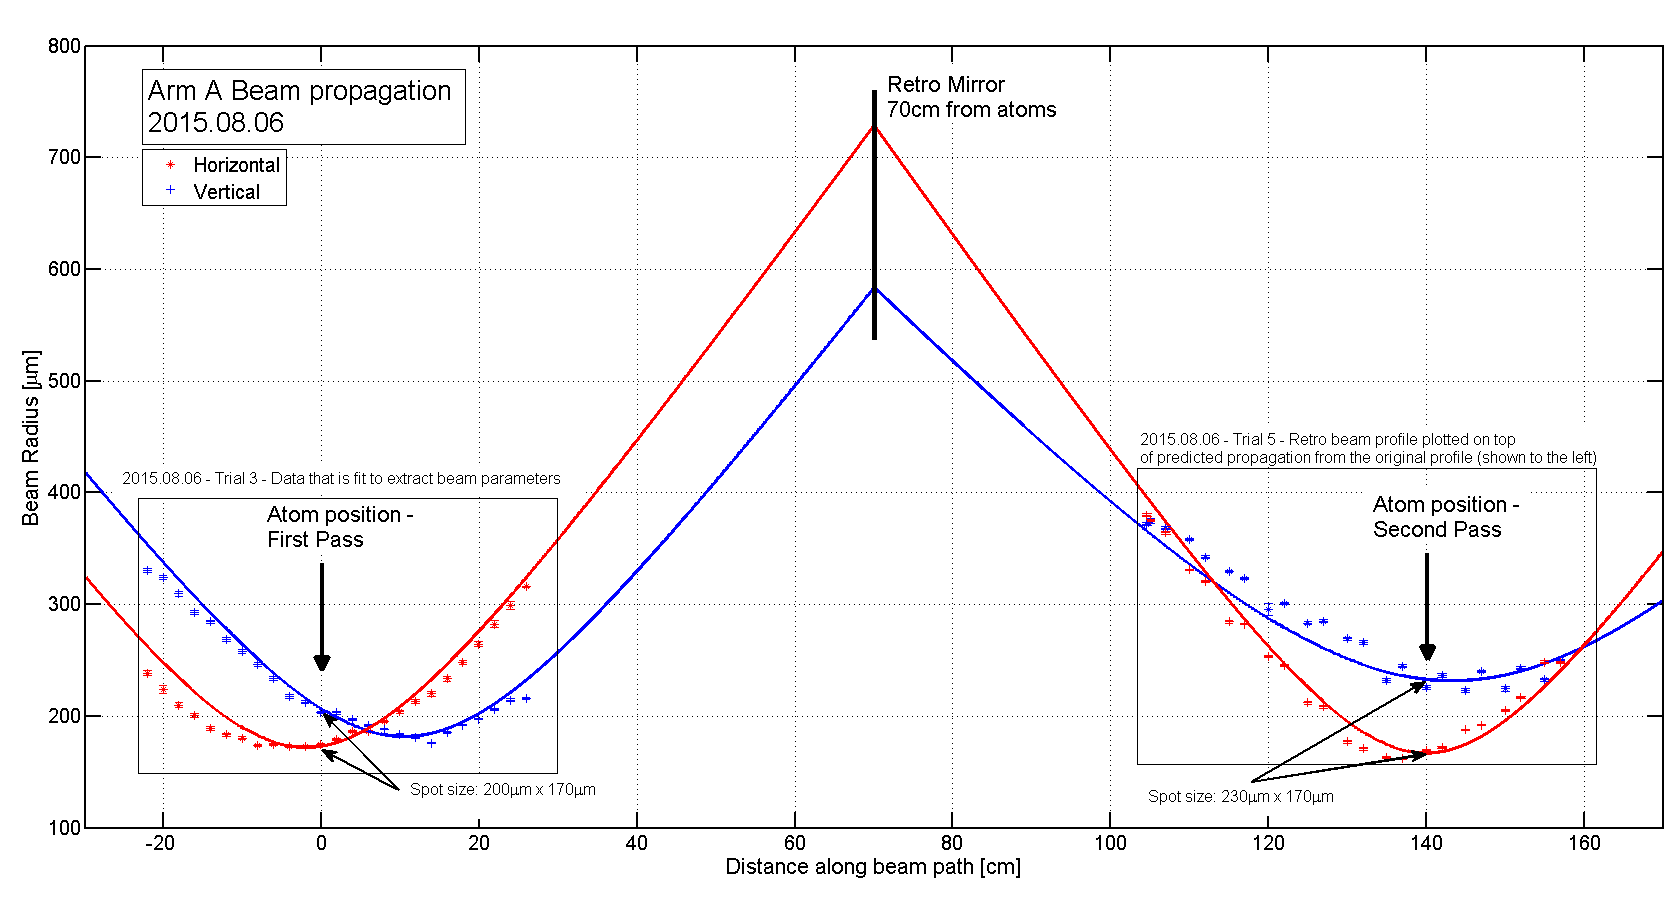
\includegraphics[width=\textwidth]{lattice_ArmAFull.png}}
		\caption{Lattice Arm A profile}
		\label{fig:532armAProfile}
	\end{figure}
	
	\begin{figure} 
		\centerline{
		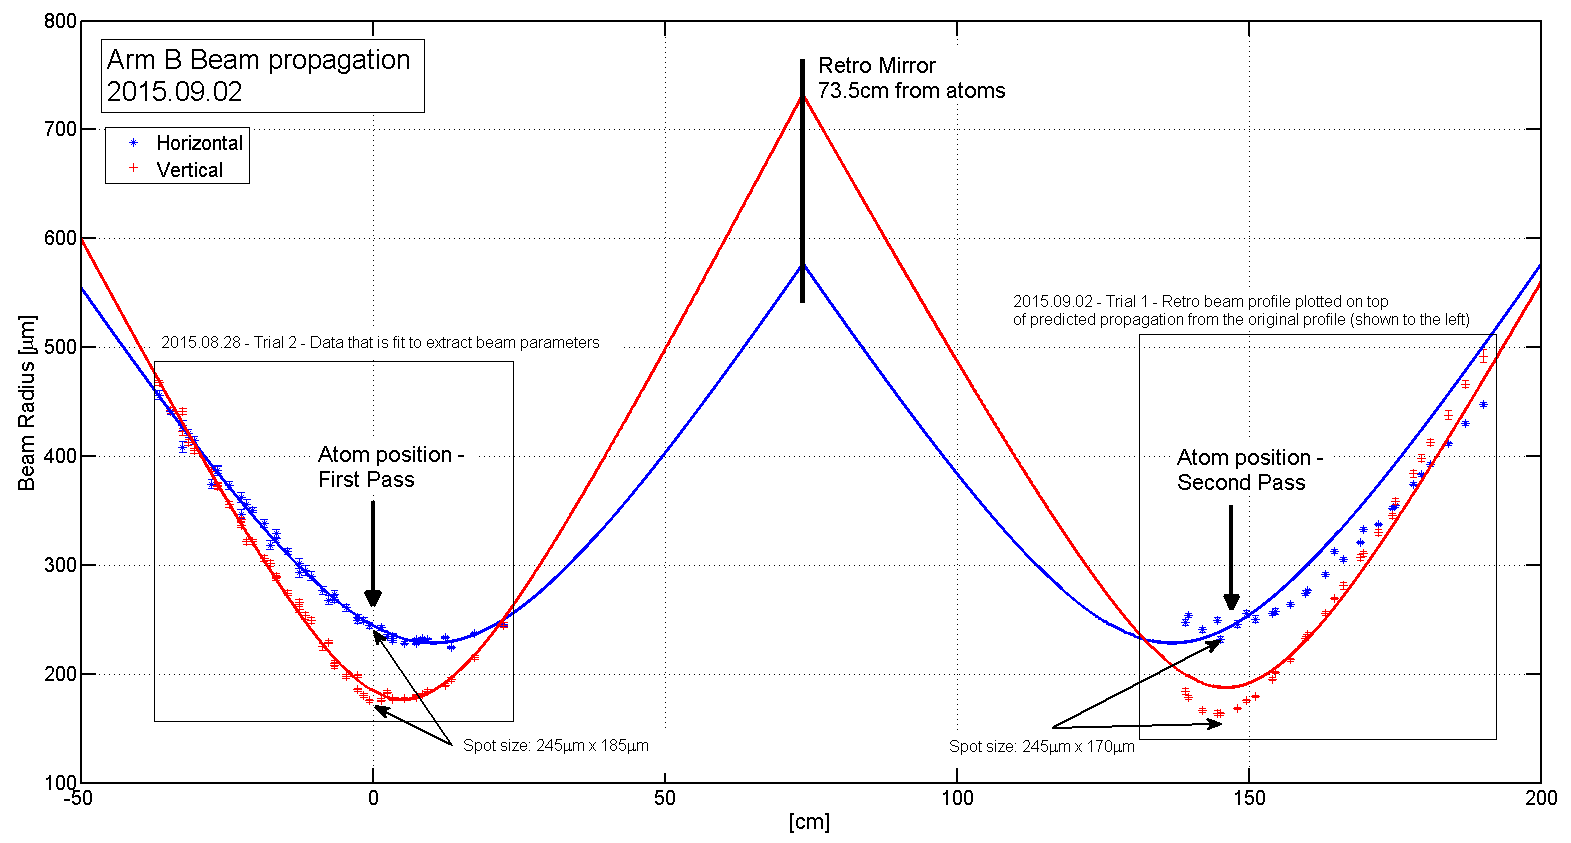
\includegraphics[width=\textwidth]{lattice_ArmBFull.png}}
		\caption{Lattice Arm B profile}
		\label{fig:532armBProfile}
	\end{figure}
	
	\begin{figure} 
		\centerline{
		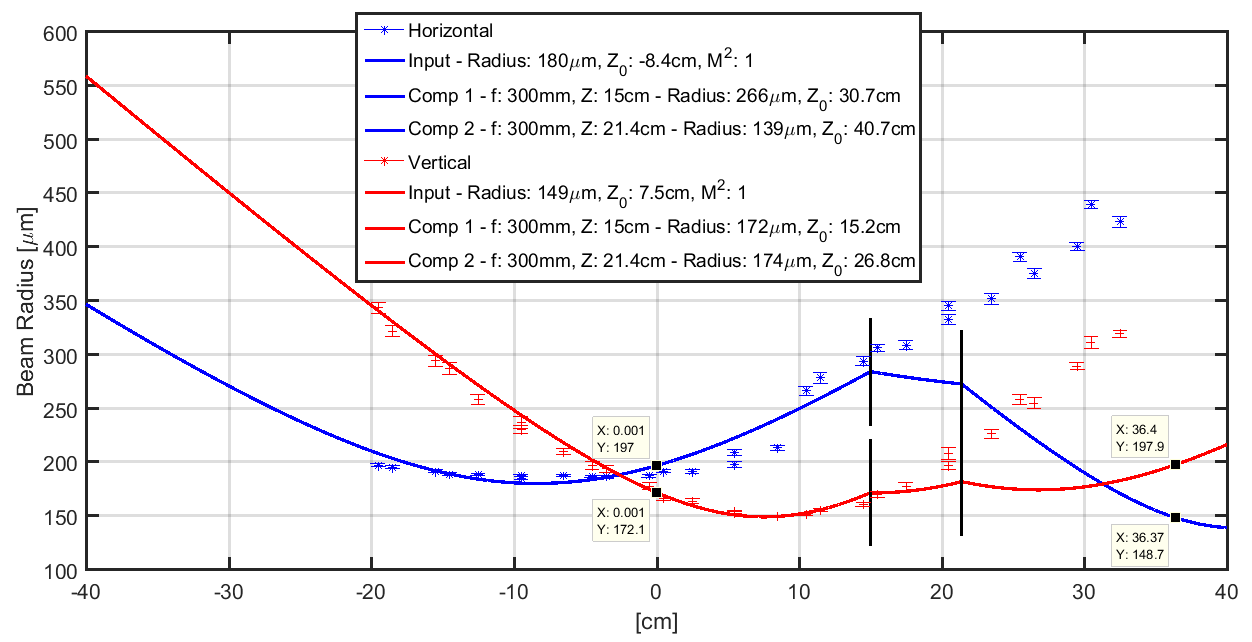
\includegraphics[width=\textwidth]{lattice_ArmCFull.png}}
		\caption{Lattice Arm C profile}
		\label{fig:532armCProfile}
	\end{figure}

\paragraph{Aligning the first pass:}
The following is a technique conveyed to our lab from Trey Porto.
We have successfully used this technique to align the first pass of the optical lattice and have found no better means of quantitatively determining the overlap of the 532 and 1064\,nm optical traps.
The basic idea is that when the beam centers are mis-aligned, the trap minima will be at a different spatial location.
Then by quickly turning off one of the beams (532\,nm in this case), we can cause quick shift in the minimum position, and thereby induce center of mass (COM) oscillates back and forth around the new minimum.
These oscillations are distinct from breathing mode oscillations where the COM stays fixed and the cloud's atoms move about it, expanding and contracting. 
These occur when the atoms are released from the lattice (though still confined to the ODT) and the new potential depth allows the atoms to pick up energy/velocity and oscillate.
We have observed these breathing mode oscillations to be present when the beams are well overlapped due to the change in trap depths (and correspondingly the potential energy of the atoms) when flashing off the 532\,nm light.

\begin{outline}[enumerate]
\1 This process requires the oscillations start from a consistent equilibrium.
We acheive this by te following experimental sequence:
	\2 Typical trapping sequence of blue MOT, repump, red MOT broadband, red MOT single frequency + ODT load
	\2 After loading the ODT, evaporate to a reasonable depth for the given loading time.
	Note that we have observed thermal effects from the ODT.
	Therefore, the point where the beam overlap should be optimized is at or near the desired trap depth for the proposed experiments.
	\2 Following the forced evaporation, hold in the 1064\,nm trap while ramp up the lattice arm being studied to full power.
	We generally find a ramp of approx. 200 - 300\,ms worked best for strontium 84. 
	\2 Once the green is at full power, we additionally held for approx. 250ms in the combined 532 + Crossed ODT trap to allow for the equilibration of the atoms in the modified trapping potential.
	\2 After the 250ms hold, the green is flashed off to excite an oscillation within the ODT.
	\2 Image the cloud as it oscillates
\1 To evaluate the procedure above, first focus on in-situ images of the cloud, where atoms are held in the combined 1064 + 532\,nm trap.
Start by moving the VI cursor positions to be on the cloud center and drawing a box around the cloud location.
This will help to identify small movements of the cloud as well as recording your start position.  
\1 When turning off the lattice and allowing the cloud to oscillate, identify the 1/4th period time of the oscillation. 
This is the point of maximum displacement and where we look to see if changes to the alignment are able to lower the oscillation amplitude.
As the alignment is improved the maximum displacement is minimized, this is the signature of improving the overlap.
If unsure about the oscillation period, scan the wait time after extinguishing the 532\,nm and observe the dynamics of the cloud to resolve a full oscillation.
\1 Each lattice arm (A,B,C) can then be varied in both dimensions (horizontal and vertical) while monitoring the oscillation amplitude. 
Lower amplitude indicates better alignment, but one must be extremely careful, as it is possible to obtain a flat signal by being so mis-aligned that the 532\,nm misses completely and no longer hits the atoms.
We have found that around the minimum in the oscillation amplitude, we are able to flip the phase of the 1/4 period oscillation as we move through the minimum.
This phase flip along with the emergence of breathing mode oscillation are robust measures of good overlap between the beams.
\end{outline}

Fig.\,\ref{fig:latFirtPass} shows an example of the above process.
Here we can clearly see that the amplitude of the oscillation is suppressed as we vary the beam pointing.
As taking this time series data is arduous, we would fix the wait time and observe the suppression as outlined above.
	\begin{figure} 
		\centerline{
		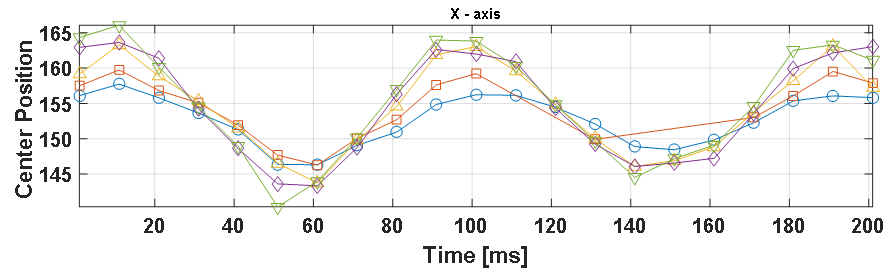
\includegraphics[width=\textwidth]{lattice_first_pass.png}}
		\caption{Center-of-mass amplitude suppression when overlapping traps}{Each subsequent scan is a single "step" in the pointing of the last mirror before the chamber. Note that the Y-axis is in arbitrary units.}
		\label{fig:latFirtPass}
	\end{figure}
	
\hl{Need to fix plot} Additional support for this method is seen in Fig.\,\ref{fig:latBreatheMode} which shows the emergence of a breathing mode when the traps are well overlapped.
In particular, we also see how reproducible this behavior is over a short time period (here about 20 minutes).
Day to day variation has not been found to be a limitation but further work must be done to ascertain the long term stability of the trap overlap.
	\begin{figure} 
		\centerline{
		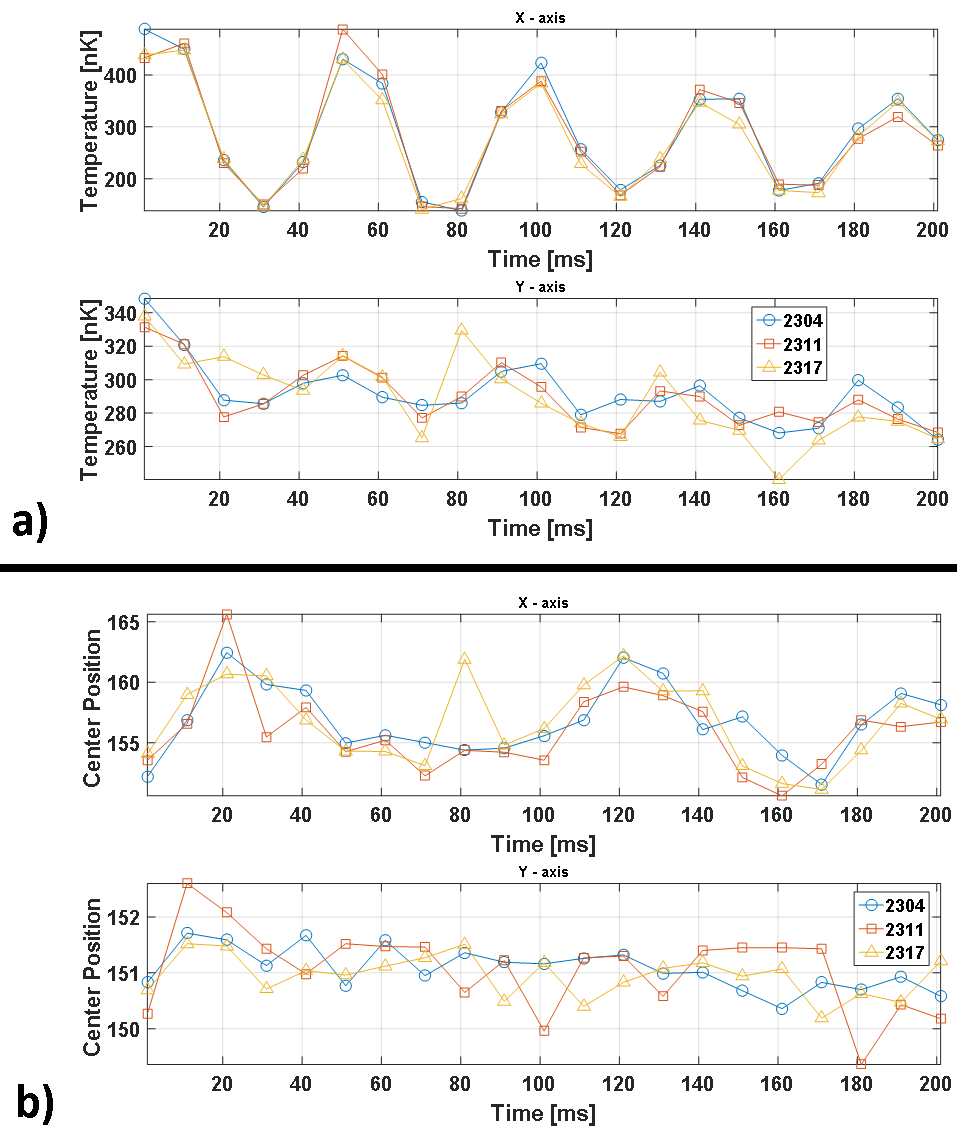
\includegraphics[height=0.8\textheight]{lattice_BreatheMode.png}}
		\caption{Emergence of breathing mode oscillation}{The measured radius and cloud centers in each axis of the absorption image. Observation of oscillatory behavior in X-axis without significant variation of the cloud center is a robust measure of the overlap of the 532 and 1064 traps. Once again, the Y-axis are given in arbitrary units.}
		\label{fig:latBreatheMode}
	\end{figure}
	
\subparagraph{Arm C:} \label{p:armCFirstPas}
The vertical path is special in all this.
We installed a special mirror as one of the last turning mirrors (give mode).
We have recently used this mirror to controllable pull the atom cloud in the 1064\,nm for performing trap oscillation measurements.
Describe using the separate program and it's limitations.
It is difficult to know we the beam is moving orthogonal to the IR beams but preliminary investigations show that small movements of the mirror axes couple predominantly along the independent IR arms.
This was deduced by performing a qualitative single point in time two-dimensional search where the in-situ cloud position was observed as the mirror position was varied.
A more quantitatively rigorous might be able to reveal the coupling between mirror axis by studying the time-series variation of the cloud center at each point of a two-dimensional mirror axis scan.


\paragraph{Aligning the retro-reflection:}
The retro-reflection is optimized via the 2-band Kapitza-Dirac method which is discussed below.
In short, for a quantum degenerate gas in shallow lattice depths, <10\,E$_r$, only the $\pm$1 plane waves will be populated.
Furthermore, for short pulses the amplitude of the population in these plane waves is linearly increasing with lattice depth.
This provides a simple single point measurement which can be used for optimizing the lattice depth.
However, an iterative approach may be needed to ensure that the alignment is only optimized during the first quarter period before the population of the orders is maximized.
Fig.\,\ref{fig:KDoscillations} shows an example oscillation.

As our lattice is free space, the first order alignment of the retro-reflection is to look over a long distance and overlap the incoming and return beam as best as possible.
This tends to overlap the two beams closely enough in the region of the atoms so as to observe some diffraction effects when performing a short high intensity pulse of the 532\,nm light.

Second, once we can observe diffraction, the gimbal mount retro mirrors are adjusted to maximize the population of the diffracted plane waves.
This alignment is extremely sensitive and may ultimately benefit from a more reproducible method of adjustment as mount backlash can strongly effect this process.
As the diffracted population is oscillatory and depends on laser intensity we have found that using an exposure time of approx 2 - 3 $\mu$s and varying the laser intensity has led to the most successful alignments of the retro.
We generally start at this short time pulse of a few microseconds with the highest intensity pulse possible and then systematically decrease the laser power into the lattice arm as the alignment is improved.
Finally we note that, as Kapitza-Dirac happens on very short timescales, the power stabilization circuits must be bypassed for this procedure.
Instead, we directly drive the RF sources with fast analog IC switches (switching time on the order of 10's ns) to apply the desired power to the lattice arm.

\subsubsection{Measurement and results}
\paragraph{Kaptiza-Dirac Scattering}
Kapitza-Dirac diffraction can be viewed as a diabatic projection from an initial eigenstate to a new set of eigenstates which results in an oscillation of the wavefunctions probability amplitudes over the new eigenstates of the system \cite{Denschlag2002}.
As was discusses in Sec.\;\ref{sec:latBackground}, the free space eigenstates are not the eigenstates of the lattice Hamiltonian. 
Thus a pure $p=0$ plane wave, $\ket{\phi_{p=0}}$, suddenly loaded into an optical lattice can be written as a superposition of the Bloch states given by Eq.\;\ref{eq:blochFunc}, here denoted by \ket{n,q}.
	\begin{equation} \label{eq:p0inBloch}
		\ket{\Psi(t=0)} = \sum_{n=0}^{\infty} \ket{n,q} \innerProd{n,q}{\phi_{p=0}}
	\end{equation}
The time evolution of this state is then given by
	\begin{equation} \label{eq:KDtime}
		\ket{\Psi(t)} = \sum_{n=0}^{\infty} \ket{n,q} \innerProd{n,q}{\phi_{p=0}} exp \left( \frac{-i E_n(q) t}{\hbar} \right)
	\end{equation}
where $E_n(q)$ is the energy of the Bloch state at a specified $q$ and $n$ shown in Fig.\;\ref{fig:bandStructure}.
The exponential factor of Eq.\;\ref{eq:KDtime} introduces oscillations among Bloch states and after a second diabatic projection back to the plane wave basis, we can relate evolution of plane wave population to the bandgap energy.
From this analysis we find that for relatively weak lattices, $V_{lat} \lesssim 10 E_r$, the plane wave population will vary as $\omega_{osc} = (E_2 - E_0) / \hbar$.
Where $E_i$ is the band energy of the i$^{th}$ band with $q=0$ as is the case when performing Kapitza-Dirac with a Bose-Einstein condensate.

Fig.\;\ref{fig:KDoscillations} shows a typical Kapitza-Dirac oscillation pattern which we use to maximize beam overlap near the atoms and calibrate our achievable lattice depths. 
Kapitza-Dirac is useful as an alignment tool since measurement of the population oscillation frequency can be highly accurate and directly relates to the bandgap energy in the lattice, shown in Fig.\;\ref{fig:bandStructure}. 
	\begin{figure}
		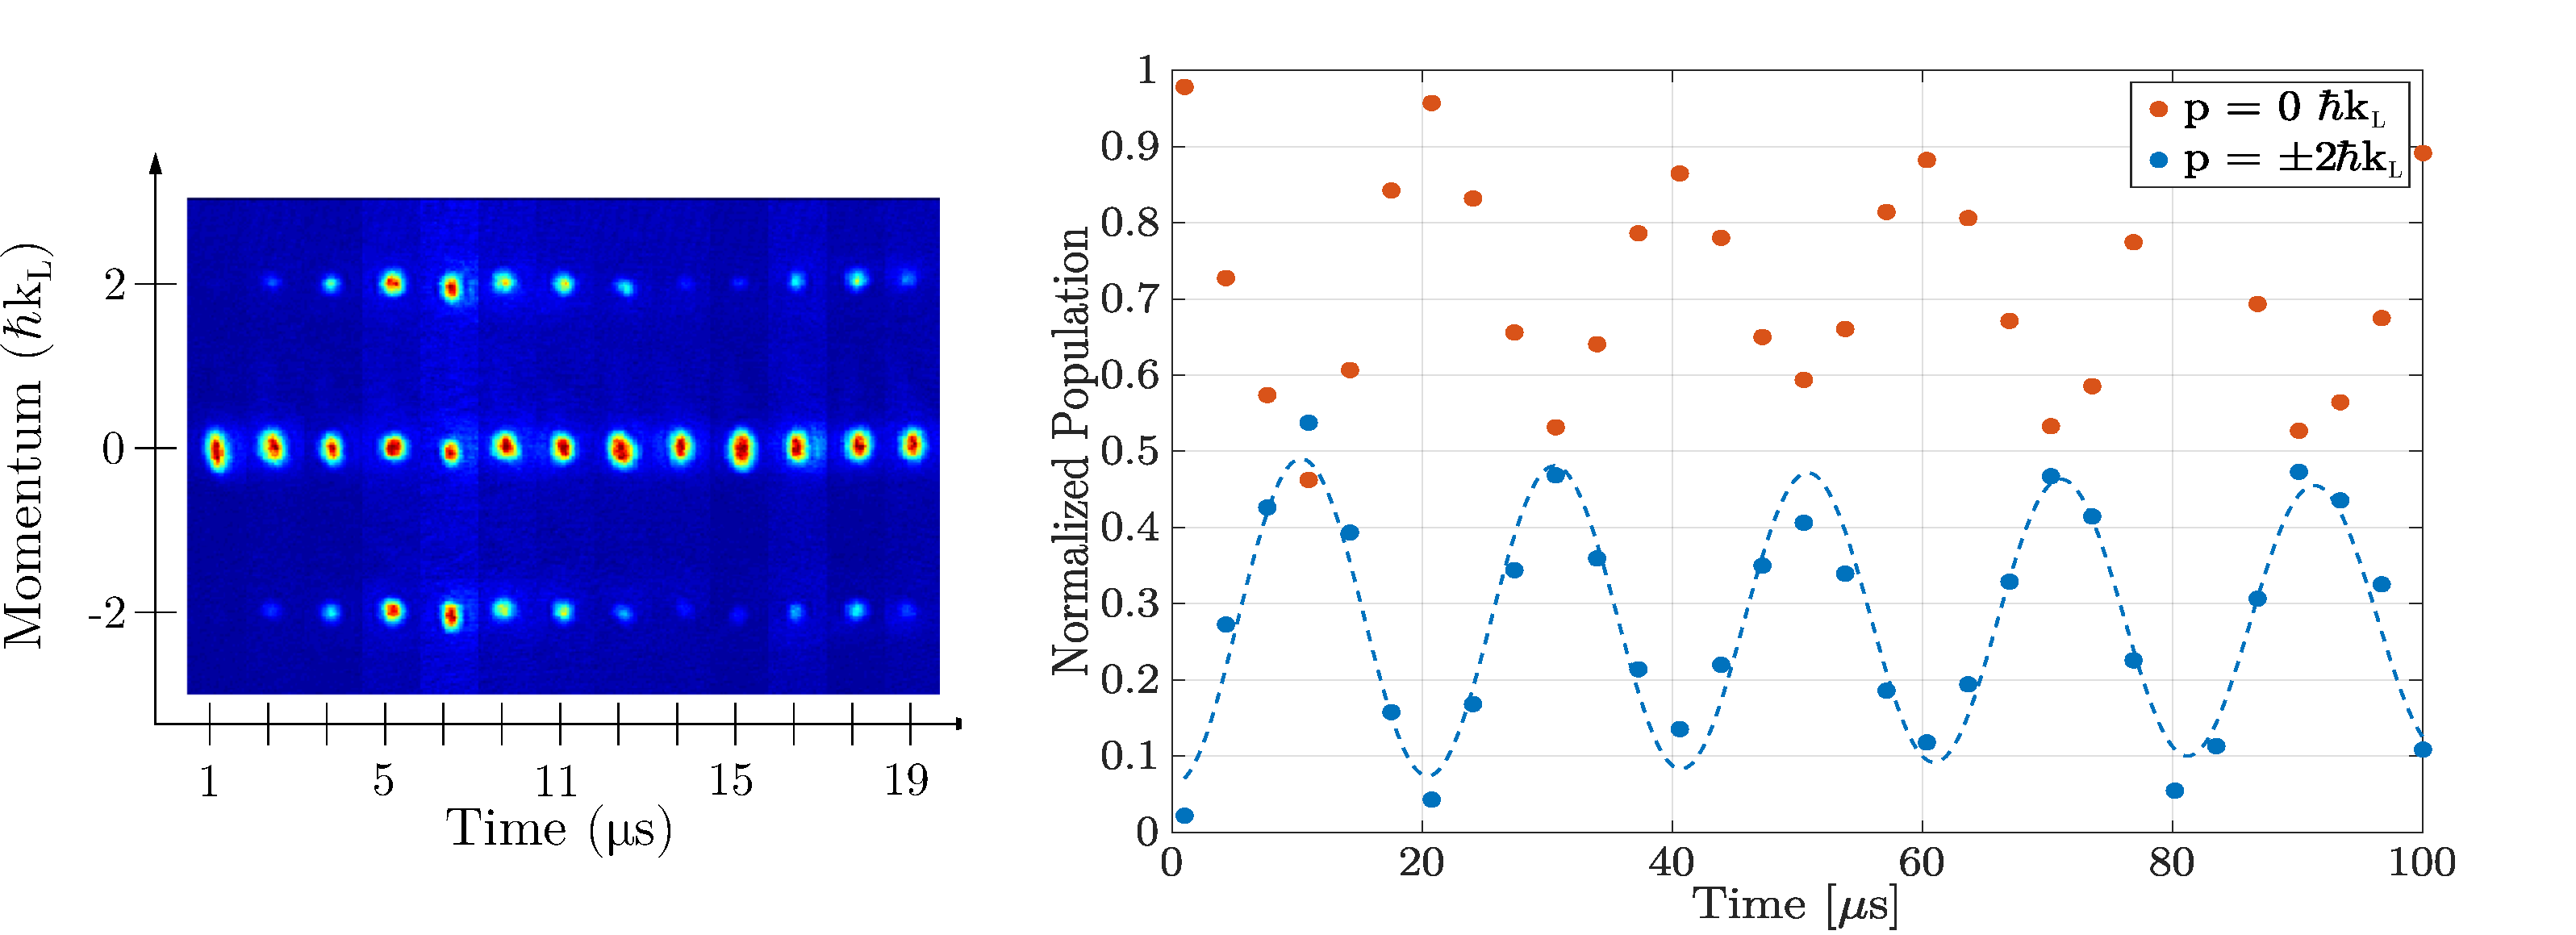
\includegraphics[width=\textwidth]{lattice_kdOsc.pdf}
		\caption{Evolution of plane wave population using Kapitza-Dirac}{Left: Time of flight slices for several realizations of Kapitza-Dirac with varying hold time in the lattice. Right: Normalized population from fits of time-of-flight images. Oscillations are fit with a decaying sinusoidal and the best-fit frequency is used to determine the lattice depth.}
		 \label{fig:KDoscillations}
	\end{figure}
	
	\begin{figure}
		\centerline{
		\includegraphics[height=0.4\textheight]{lattice_1DOscPeriod.png}}
		\caption{Oscillation period between $n=0\,\rightarrow\,n=2$ band at $q=0$}
		\label{fig:latOscPeriod}
	\end{figure} 
For reference, Fig.\,\ref{fig:latDepth} shows the resulting lattice depth calibration for our most recent alignment.
	\begin{figure} 
		\centerline{
		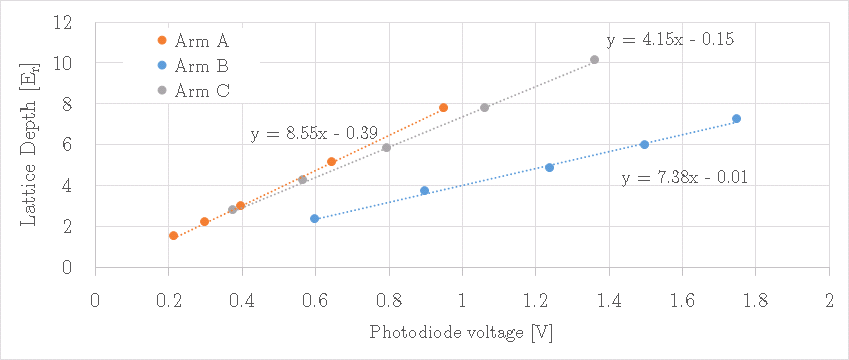
\includegraphics[width=\textwidth]{lattice_depth.png}}
		\caption{Lattice depth calibration}{Calibration was performed using the two-band Kapitza-Dirac technique. Maximum photodiode voltage for each arm is 10\,V}
		\label{fig:latDepth}
	\end{figure}
	
\subparagraph{Higher order Kapitza-Dirac:}
The simple two-band model given above is a straightforward method for determining the lattice depth but one that requires a time-series measurement over varying lattice depths.
Gadway et. al. \cite{Gadway2009} derived a complimentary depth calibration method which requires only a single time-series measurement at high lattice depth.
This process relies on the quantum interference of the oscillating populations which produces a complex beat note.
An undergraduate report from Alex Wikner \cite{Wikner2017}, follows the original Gadway construction to develop an algorithm using Matlab$^{TM}$ for applying this technique to the Neutral apparatus.
The cited report provides sample code as well as benchmark calculations for comparison.
However, application of this work to calibrate the lattice depth has been stymied by a consistent heating concern we have observed when applying the lattice beams for significant periods at high lattice depths.

\paragraph{Heating of a quantum degenerate gas}
While Kapitza-Dirac diffraction is useful as a characterization tool, we typically wish to maintain equilibrium when loading condensates into the lattice. 
Thus slowly ramping up the lattice laser intensity will adiabatically transform a plane wave ground state into the ground Bloch state of the lattice \cite{Sakurai2010}. 
Strictly speaking, in order to adiabatically connect the free space eigenstates and the lattice eigensates, the lattice must be turned on infinitely slowly due to the infinitesimal bandgaps which open near the band edges. 
Although near the band center, $q=0$, the adiabaticity requirement relaxes to $dV_{lat}/dt \ll 16E_r^2/ \hbar$, \cite{Denschlag2002} which for strontium in a 532\,nm lattice is $\approx 5\,\mu$s$/E_r$. However, in practice we find that our condensate fraction is reduced during fast ramps into the lattice. 

Instead, we slowly ramp on the lattice over 100\,ms which reduces heating caused by the ramp. 
We have experimented with various functional forms of this pulse shape and currently rely on an S-shaped curve given by Eq.\hl{somthing}.
\begin{equation}
	tanh
\end{equation}

As shown in Fig.\;\ref{fig:heatingRates}, we observe a large condensate fraction after similarly ramping the lattice back down. 
Additionally, by holding in a deep lattice after an adiabatic ramp, we can measure the effects of off-resonant scatter of lattice photons as a reduction of atom population over time.
For our red detuned optical lattice we expect the off-resonant scattering rate to be well approximated by a simple two level approach. In this model, the effective scattering rate is given by \cite{Jaksch2005}
	\begin{equation} \label{eq:offResScatter}
		\Gamma_{eff} \approx \frac{\Gamma V_{lat}}{\hbar \delta_{lat}}
	\end{equation}
where $\Gamma$ is linewidth of the dipole transition between the two states, $V_{lat}$ is the lattice depth, and $\delta_{lat}$ is the detuning of the optical lattice from the two level transition frequency.
In strontium, the $^1S_0\!\rightarrow\!^1P_1$ transition strongly dominates the polarizability of the ground state and therefore can be used to estimate the effective off-resonant scattering rate.
For this transition $\Gamma = 2 \pi \times 30.5\,$MHz and a 532\,nm lattice is detuned by $\delta_{lat} \approx 2 \pi \times 87\,$THz.
With a lattice depth of $V_{lat}=10\,$E$_r$ we expect a scattering rate of $\Gamma_{eff} \approx 2\e{-1}\,$s$^{-1}$, which is negligible for the timescales of our proposed experiments.
From Fig.\;\ref{fig:heatingRates}, we see that there is not an appreciable loss of atoms over a one second timescale, which at first would support our estimate that off-resonant scattering is unimportant on these timescales.
	\begin{figure}
	\centerline{
		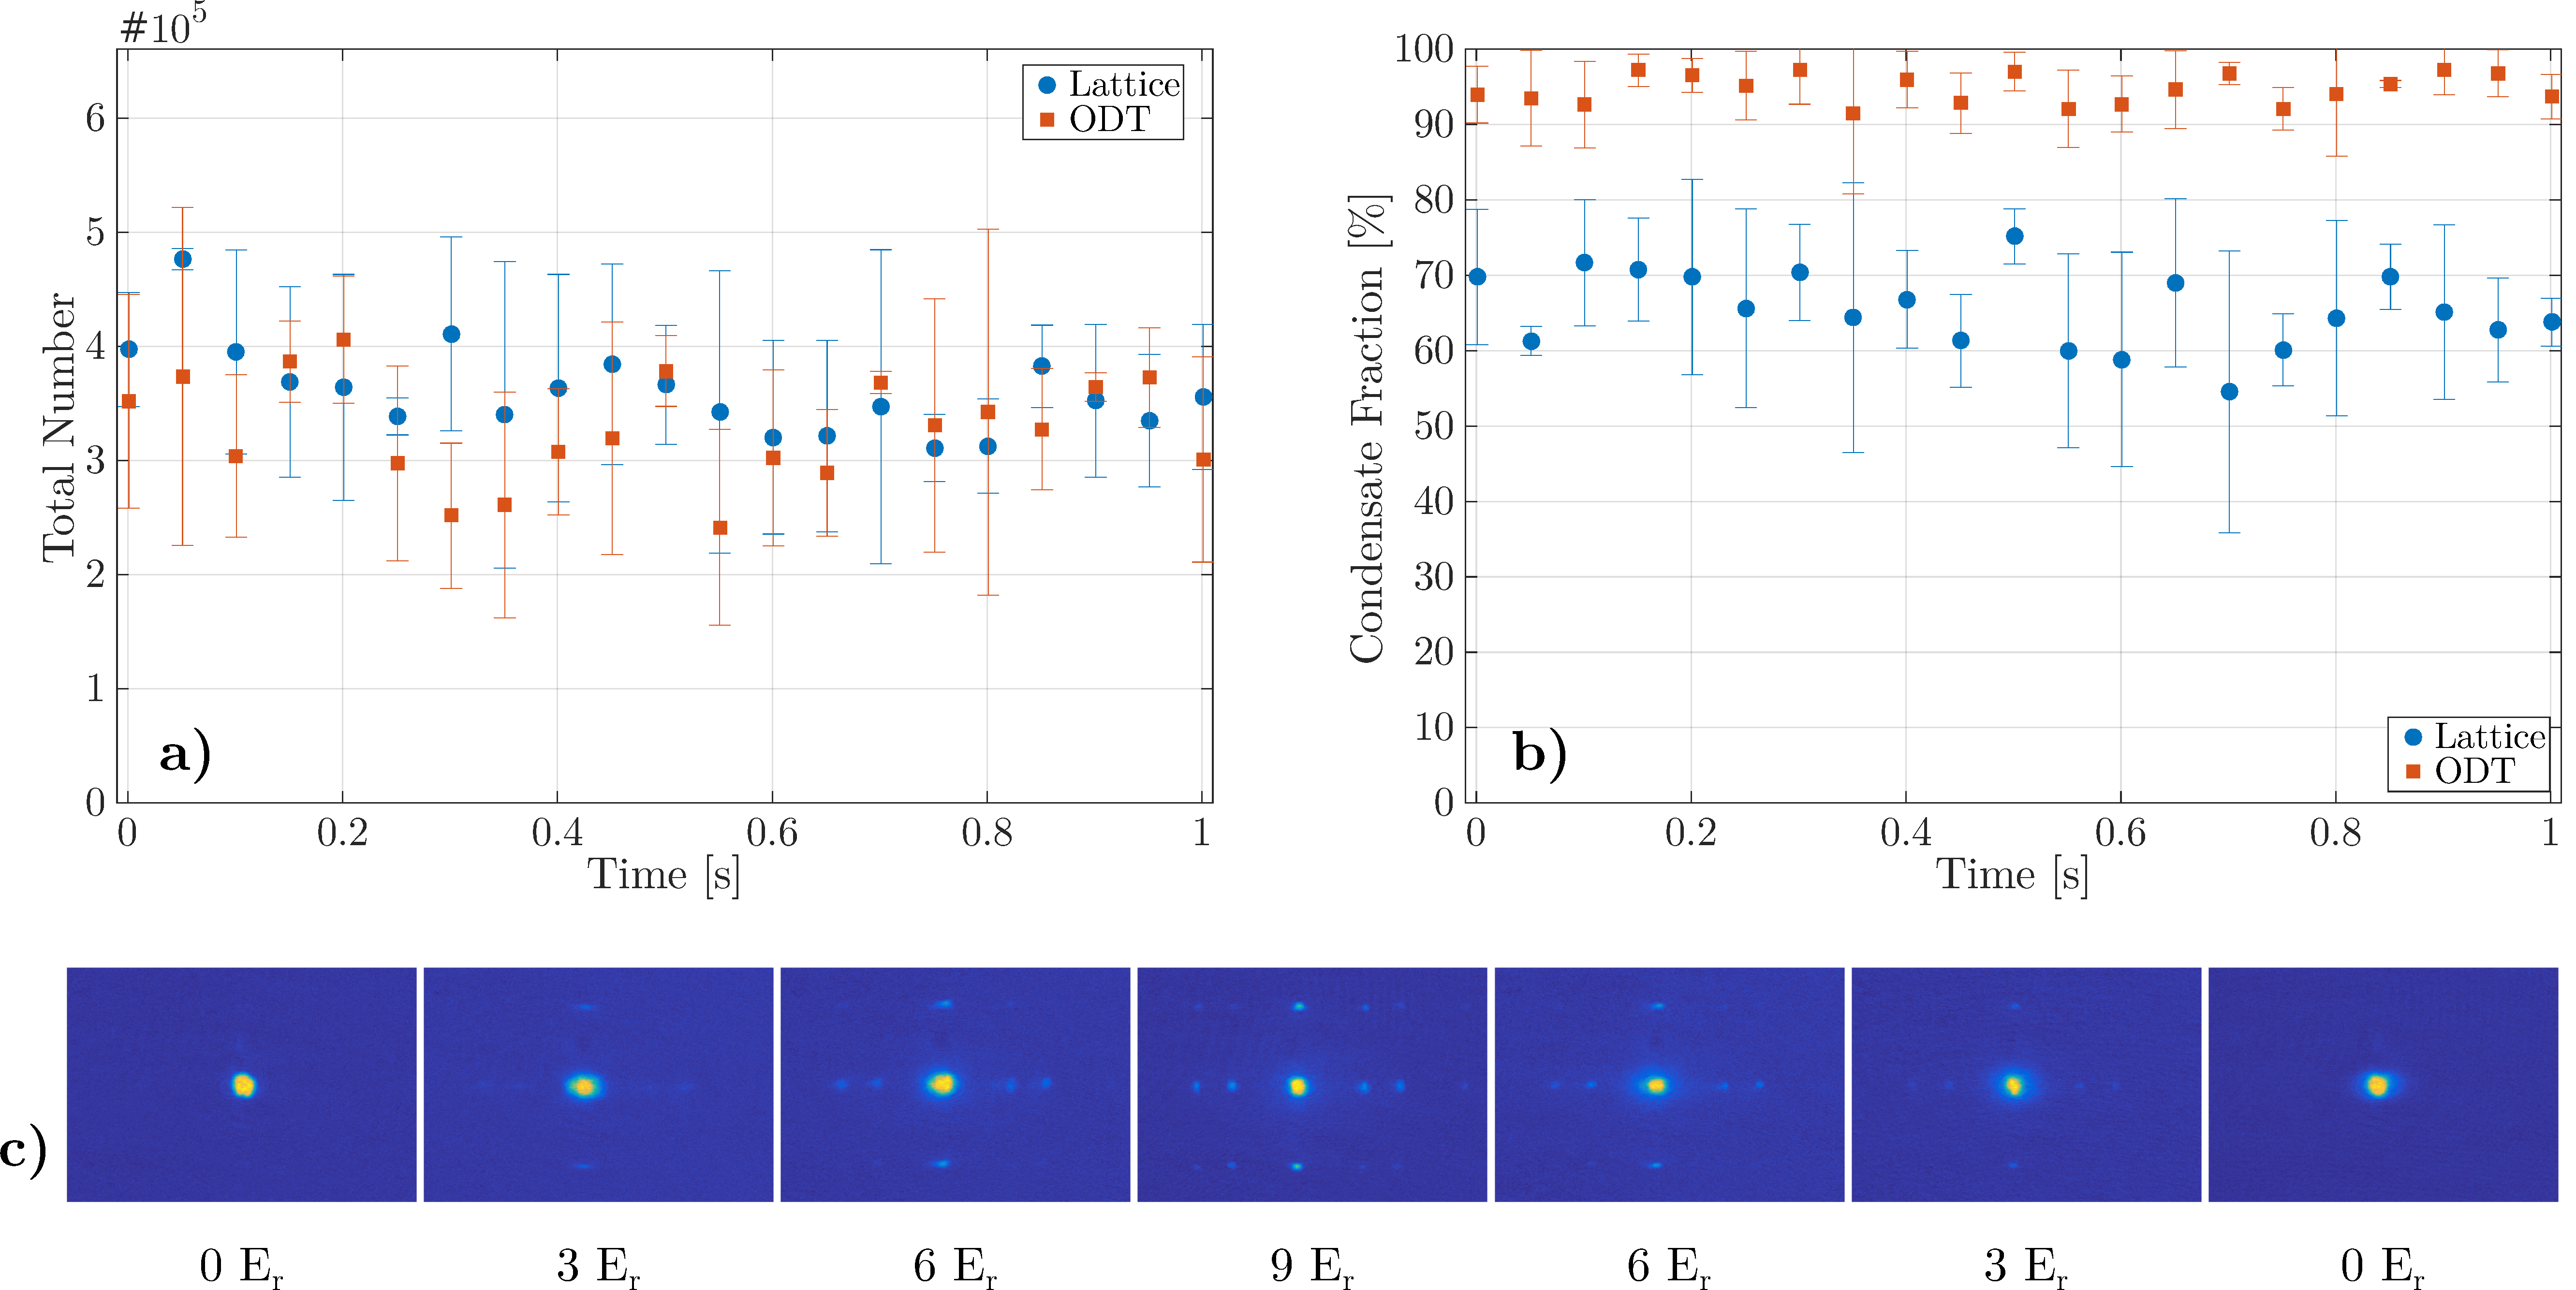
\includegraphics[width=\textwidth]{lattice_heatRates.pdf}}
		\caption{Characterization of heating in the optical lattice}{Evolution of condensate fraction over time after adiabatically ramping on the lattice to 9\,E$_r$. a,b) Comparison of total number and condensate fraction for a sample held in the optical dipole trap (red squares) or in a deep lattice (blue circles). c) Time of flight images after ramping on the lattice and diabatically projecting back to plane wave states.}
		 \label{fig:heatingRates}
	\end{figure}
Unfortunately, we have recently found that attempts to load a degenerate gas into a deep lattice, $\gtrsim 10$\,E$_r$, leading to unacceptable heating of the atomic sample.
Currently, we hypothesize that this may result from the freespace nature of the lattice or an intrinsic instability (frequency or power) of the Verdi.
The latter of these has been tested by monitoring the 532\,nm light in a spectrum analyzer where no obvious deficiencies have been observed.
To test the former hypothesis, we are currently investigating fiber coupling one of the arms of the lattice but as of spring 2019, this project is ongoing.

\subsection{Optical toolbox} \label{ssec:op_tools}
\subsubsection{Absorption imaging system}
Absorption imaging is a destructive measurement process which is predicated on measuring the spatially distributed attenuation of laser light after passing through an atomic cloud. 
In this section we will discuss the technical details of the Neutral absorption system and reserve the theoretical description of the process to Sec.\,\ref{ssec:tof}.
Additionally, we will reserve the discussion of image processing for App.\,\ref{app:imagefitManual} which details our software used to analyze the images and extract our physical measurements.

Fig.\,\ref{fig:absImagingSchematic} shows a simplified schematic of the absorption imaging system.
	\begin{figure} 
		\centerline{
		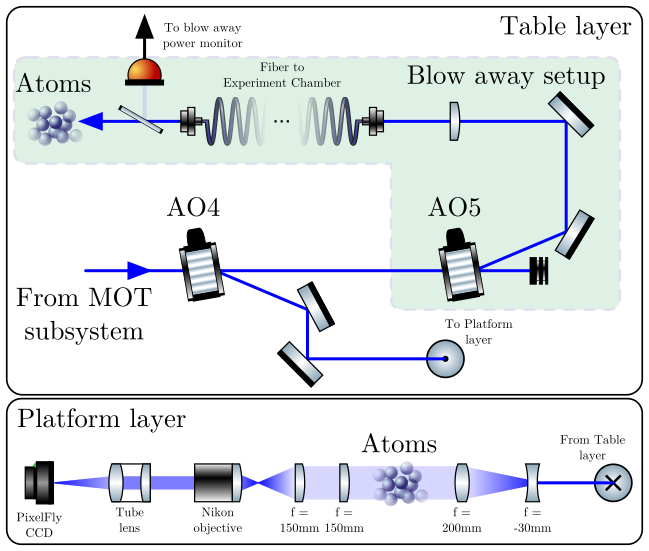
\includegraphics[width=0.8\textwidth]{461_imagingSchematic.png}}
		\caption{Absorption imaging and blow away pulser optical schematic}{Details on the contrsuction and characterization of the blow away setup are available in Josh Hill's masters thesis \hl{ref}.}
		\label{fig:absImagingSchematic}
	\end{figure}
Light is derived from the MOT path sub-system and guided to the atom chamber via freespace propagation. 
After passing through the atoms an imaging system shapes and focuses the image onto a Cooke PixelFly CCD camera.
The PixelFly is a 12\,bit 1280x1024 CCD with a pixel size of 6\,$\mu$m.
The imaging system after the atomic sample was developed by Mi Yan and is outlined in detail in App. A of his PhD thesis \cite{Yan2013d}. 
Much of the imaging sequence is a standard procedure that does not change day to day.
However, there are a couple of technical issues that may affect the operation of this system which we'll outline below.

First, it is important to not overexpose the image through saturating the camera's pixels by applying the imaging laser for too long.
We typically expose for 5\,$\mu$s with sample optical depths around one.
Due to drifts in the power output of the MOT cavity, we must occasionally increase the exposure time.
The figure of merit for determining the exposure time, is to expose just below saturation around the edges of the image\footnote{The auto-ranging color axis in the Labview VI is useful for quantitatively determining what the maximum pixel count is, then just keep it near but just below $2^{12}=4096$}.

The second consideration when taking images is related to how we extract the optical depth from images, the physics of which is discussed in Sec. \ref{something}.
For now, we will take as a given that each experimental sequence requires one image with the atoms in frame and another background image without the atoms.
In the ideal scenario these two images would be identical except in the region of the atom cloud and thus information about the cloud could be inferred using Beer's law \hl{ref}.
However, practically we must wait for the atoms to exit the frame and thus introduce a time delay between between the consecutive images that we seek to minimize.
For this reason we utilize a special feature of the PixelFly called "double-shutter" mode.
This particular imaging mode of the camera utilizes a second hidden set of pixels that are interleaved with the active pixels of the CCD.
Typically the acquisition time between consecutive images taken with a CCD is limited by the analog-to-digital conversion time needed to readout the image from the pixels into the camera's memory.
However, the PixelFly's set of hidden pixels lets the first image that is taken simply shift one row down from the active pixels into the hidden ones once the externally triggered exposure time has elapsed.
Once shifted down, the active pixels are free to be exposed again.
With this process the time between images is reduced to 5$\mu$s.
Fig.\,\ref{fig:pixelflyTiming} shows a full overview of this process.
	\begin{figure} 
		\centerline{
		\includegraphics[width=0.6\textwidth]{misc_pixelflyTiming.png}}
		\caption{Timing diagram of PixelFly doubleshutter mode}{t$_j$ refers to timing jitter inherent to the camera. In this scheme the first exposure can be controlled via the external trigger but the second image exposure is fixed to the readout time of the first image.}
		\label{fig:pixelflyTiming}
	\end{figure}
The drawback of this scheme is that for exposure times less than the readout time of an image, the second image is forced to have a minimum exposure of the readout time.
This presents a challenge as our exposure time is about four orders of magnitude faster than the readout time.
To overcome this, we rely on the fast response of the imaging system AOMs, a high extinction ratio of the 461\,nm photons, and a narrow line filter centered at 461\,nm attached directly to font face of the CCD.
Fig.\,\ref{fig:absImagingSchematic} shows two AOM's along the imaging path before the atoms.
We found two AOM's necessary to attenuate leakage light along the path to acceptable levels while maintaining fast response times which a physical shutter cannot replicate.

Great care is taken to reduce the time between images since the laser intensity and frequency might drift between the atom and background images. 
Variations in intensity have straightforward implications for errors since the measurement of the atomic number density assumes the only difference between the images is due to the presence of scattering particles, Sec.\hl{some sec}, and does not account for fluctuating photon number. 

The more insidious source of error in absorption imaging is variation of the optical frequency. 
Coherent, frequency stabilized radiation is used to illuminate the atom cloud so that we may control the optical absorption cross section and accurately measure the atomic number density. 
However, this laser light is passed through many optical components on it's path to the atoms and ultimately the imaging camera. 
Small reflections along this path result in a multitude of interferometers which causes small scale spatial intensity variation across the beam. 
Exacerbating this problem are short time frequency drifts that may occur between the atom and background images which result in slightly different fringe patterns in the atom and background images. 
Fringes patterns are a well known nuisance in experimental AMO images and it has become routine to use linear algebra techniques (PCA, ICA, etc.) to create a composite background image for each atom image during analysis \cite{Segal2009} in order to create a higher quality image of the optical depth.. 
A brief discussion of the principal component analysis (PCA) algorithm employed by the Neutral analysis routine is outlined below, while a more discussion can be found in Sec. \hl{some sec}. 

Briefly, the PCA approach is as follows:
\begin{outline}[enumerate]
	\1 Find a basis set of background images from a large set of raw background images.
	\1 For a single atom image, construct an initial guess at a composite background image using coefficients to weight each basis image resulting in a superposition of the basis images.
	\1 Segment the atom image into multiple regions by separating out the region of interest around the atom cloud.
	\1 Comparing similar regions between the composite background and the atom background region, perform a least-squares minimization by varying the weighting coefficients of the composite background.
	\1 Once a suitable composite background has been found, calculate the optical depth using the atomic region of interest and the corresponding region of the minimized composite background image.
\end{outline}
This procedure is repeated for each atom image using a static background basis set that is computed for each scan.
Fig.\,\ref{fig:PCAcomp} shows an example of using this technique with a background set of 20 other images (not shown).
	\begin{figure}
	\centerline{
		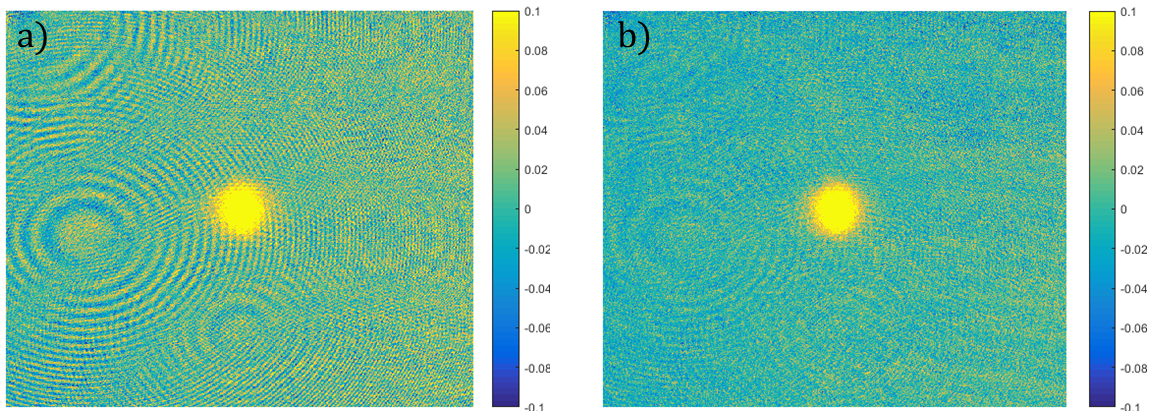
\includegraphics[width=\textwidth]{misc_PCAcomp.png}}
		\caption{Comparison of background subtraction methods}{Background subtraction on the same image performed using two different methods and plotted on the same color scale. a) The partner-in-time background to the atom image is used. b) A composite background image formed via PCA is used.}
		 \label{fig:PCAcomp}
	\end{figure}
While PCA does not completely eliminate the visible fringe patterns, there is a noticeable reduction of the fringes in the PCA image versus the partner-in-time method.

\subsubsection{Highly tunable 689\,nm spectroscopy system}
The spectroscopy laser is derived from a dedicated slave diode and is our primary 689\,nm probe for bosonic isotopes, with the spin manipulation laser described below being used for fermions.
This laser system is used for general intercombination line spectroscopy, photoassociation, Bragg scattering, and Rabi oscillation measurements.

Fig.\,\ref{fig:689specSch} shows a simplified optical diagram.
	\begin{figure}
	\centerline{
		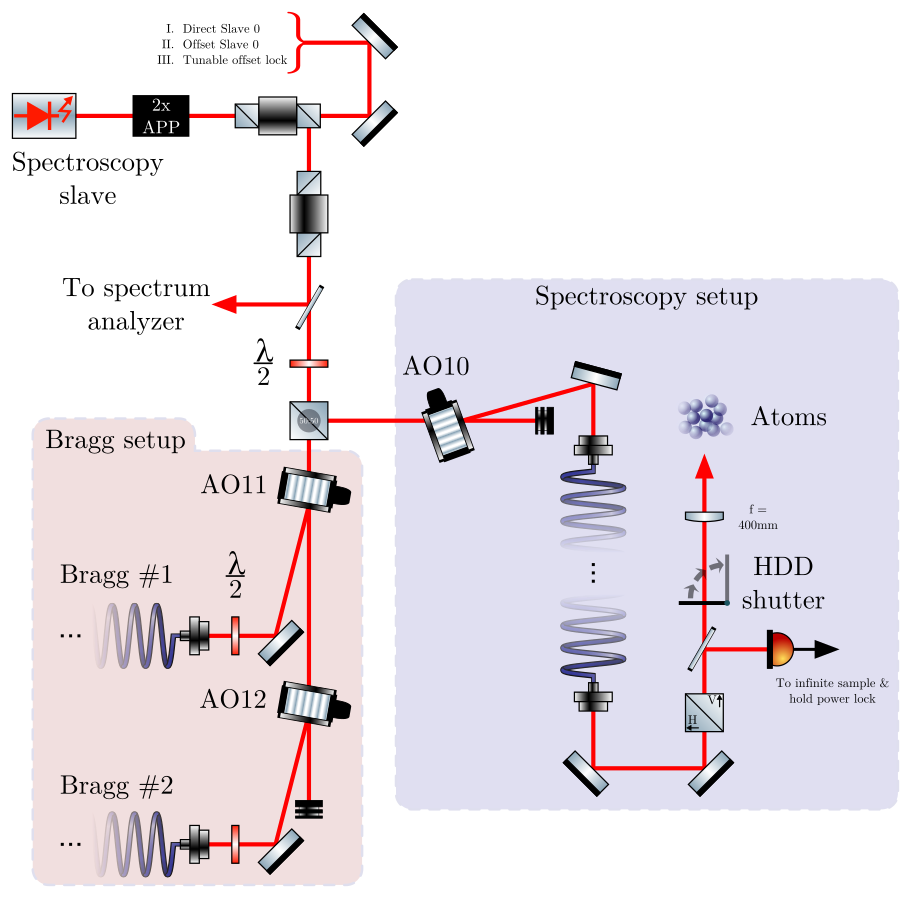
\includegraphics[width=\textwidth]{689_specSlaveSchematic.png}}
		\caption{Optical schematic: 689 spectroscopy laser}
		 \label{fig:689specSch}
	\end{figure}
We found it necessary to increase the isolation out of the laser as the injection lock became unstable when coupling into the fiber couplers due to back reflections.
We typically get $\sim25$\,mW of usable power past the second isolator.
As this is our primary spectroscopy laser, its optical setup tends to be in flux but a couple of noteworthy innovations have been implemented in recent years.
These include the development of an infinite sample and hold for intensity stabilization, a versatile injection locking scheme, and a shallow angle Bragg scattering setup.

The infinite sample and hold (ISH) circuit is used in conjunction with an intensity stabilization lock circuit and was built to allow for intensity stabilized "chirped" pulses on timescales much faster then the acquisition time of the intensity lock circuitry, typically $\sim70$\,ms.
This circuit was developed and built by Josh Hill and is based on the LTC1417 which is a low power 14-bit 400\,kS/s ADC.
Details of the circuit construction and characterization are left to Josh's forthcoming thesis.
The ISH is currently placed on our spectroscopy probe and is situated between the intensity stabilization lock circuit and RF voltage controlled attenuator.
This allows the ISH to passively sample the control voltage from the lock circuit.
In sample mode the ISH output follows the input from the lock circuit.
When the ISH is transitioned into hold mode, it begins ignoring changes on its input and outputs the last voltage that was sampled before the transition.
A timing disgram of the infinite sample and hold usage is outlined in Fig.\,\ref{fig:689specInfSH}.
	\begin{figure}
	\centerline{
		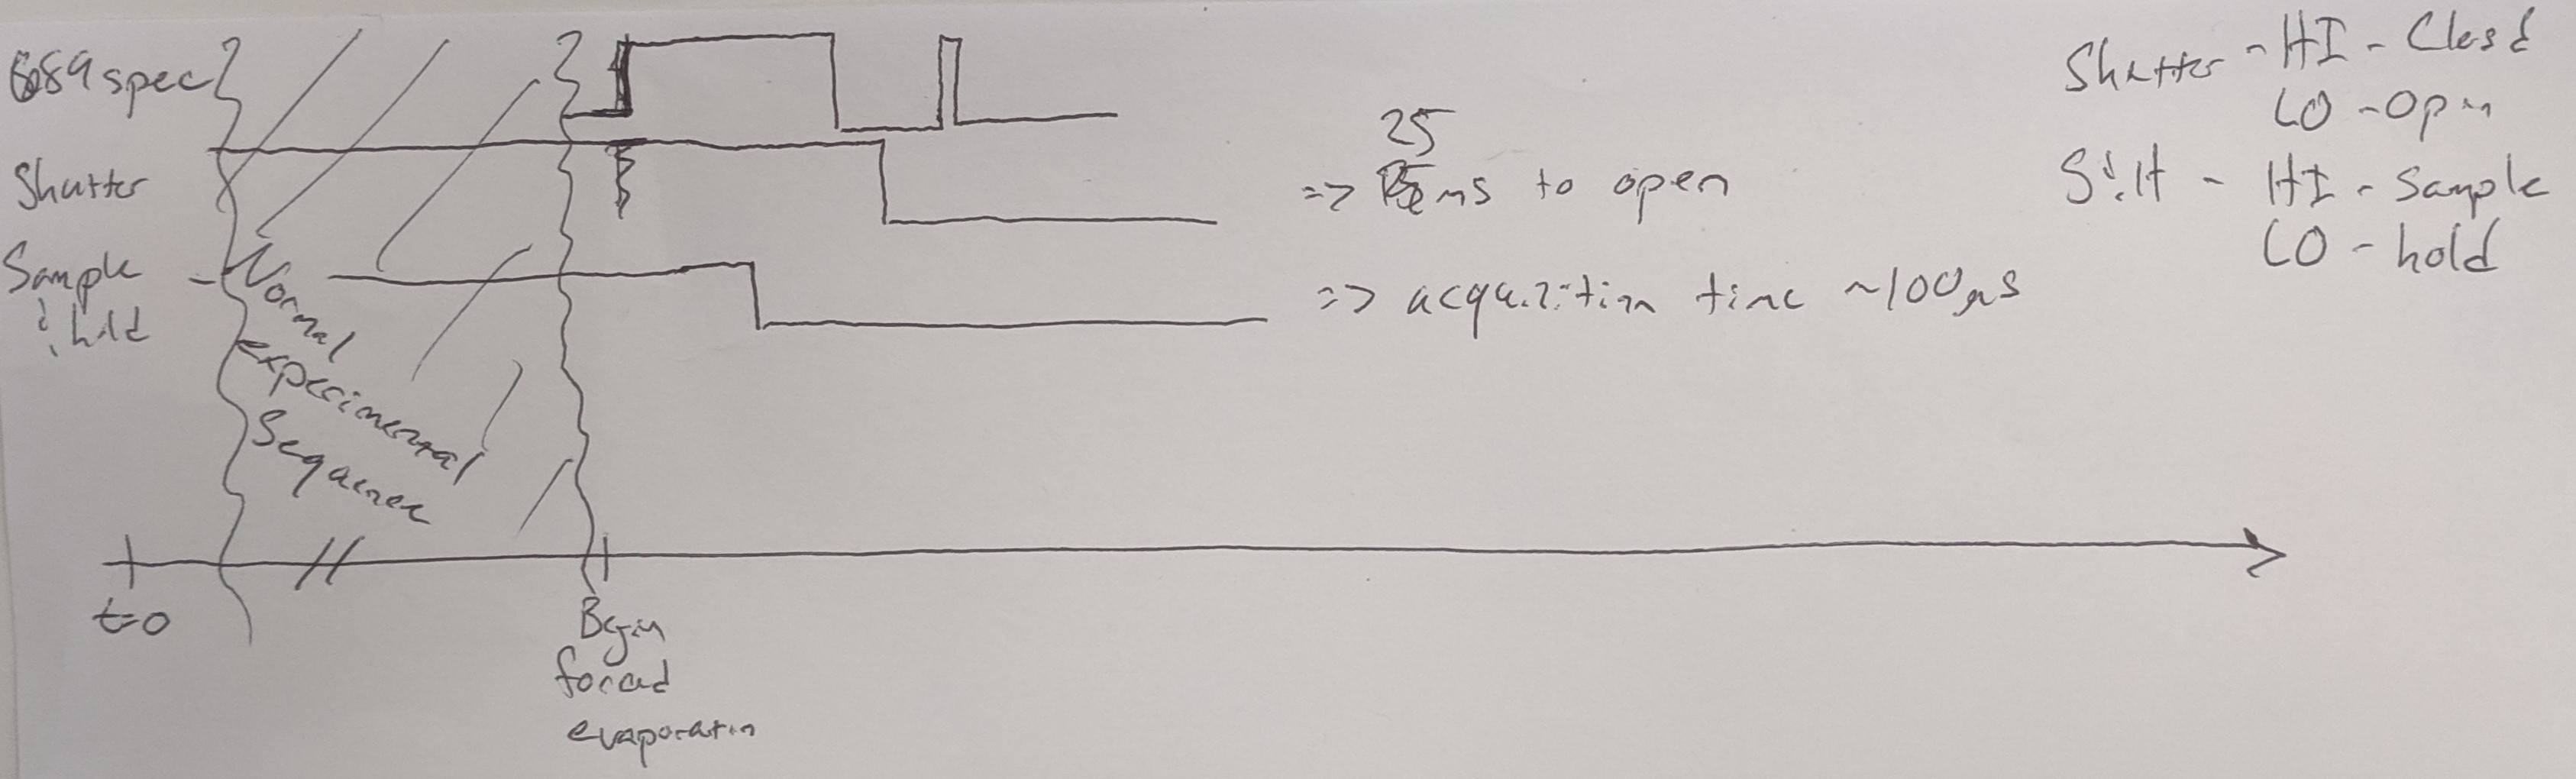
\includegraphics[width=\textwidth]{689_specInfSH.jpg}}
		\caption{Infinite sample and holding timing diagram}{The HDD shutter in use has a full open time of $\sim15$\,ms and the acquisition time of the sample and hold chip is on the order of $\sim500ns$.}
		 \label{fig:689specInfSH}
	\end{figure}
Following our typical preparation sequence we place the ISH in sample mode and enable the spectroscopy probe with the HDD shutter blocking the beam. 
This allows the lock circuit time needed to acquire and stabilize the feedback voltage required to maintain the current intensity setpoint.
Following lock acquisition, we transition the ISH into hold mode, open the shutter, and pulse the RF onto the spectroscopy AOM (AO10) via a fast RF switch (model: Mini-circuits ZASWA-2-50DR+) where the RF amplitude is attenuated via a voltage controlled attenuator and the voltage input is the fixed output value from the ISH.
This momentary transition to open-loop operation of the intensity stabilization circuit does suffer from slow long term fluctuations shot to shot, but does provide a marked improvement on the intensity reproducibility without placing restrictions on the minimum pulse time required.
Furthermore, by monitoring and recording the slowly varying intensity fluctuations, we can model any error introduced by the reduced intensity variation.

Another notable improvement has been the versatile injection locking scheme for varying the frequency of the spectroscopy slave with respect to the maser laser.
This scheme allows us to change the seed laser frequency via three different methods outlined below.
\begin{outline}[enumerate]
	\1 Directly following slave 0
		\2 A small amount of light from slave 0 is coupled directly into the rejected port of the spectroscopy slave, resulting in the frequency of spectroscopy slave and slave 1 being shared. 
		Fig.\,\hl{something} shows the position of this pick-off before the boson red MOT AOM. 
		Recalling that slave 0 is always positioned +82\,MHz of the bosonic isotope of interest, the direct method will position the frequency of the spec. slave to also be +82\,MHz.
	\1 Slave 0 minus 40\,MHz
		\2 The light sent from slave 0 is shifted down 40\,MHz by the spec. offset AOM. This positions the spec. slave frequency at +42\,MHz of the intercombination line of interest.
	\1 Programmable offset
		\2 In 2018 we re-purposed the original homemade 689 master ECDL described in Natali's thesis as a slave ECDL and directed light from this setup as a tertiary method for tuning the frequency of the spec. slave. 
\end{outline}
There are several things to note concerning the above descriptions.
First, to reiterate, the "of interest" designation specifically refers to the variability of the laser frequency of slave 0 which is dependent on the configuration of the isotope selector AOM as discussed in Sec. \hl{somewhere}.
Second, switching between case I and II is surprisingly trivial given the realized setup on the table.
In practice, a flipper mirror and clever optical path alignment allow us to switch between these two injection methods in a matter of seconds and has demonstrated remarkable stability.
Thirdly, while the programmable offset is the most versatile of the presented schemes, it also has the greatest frequency uncertainty and is fundamentally a different approach that we are still in the process of exploring.

The slave ECDL, beatnote generation, and phase locked loop (PLL) integrated circuit was a project begun by a visited student and later completed by Josh Hill.
We will leave the detailed description of the Neutral implementation for Josh's forthcoming thesis and instead reserve our current discussion to an overview of the technique.
It is based on the 2009 work of Appel et. al. \cite{zfr08expansion} which outlines a versatile optical phase locked loop with a claimed frequency range of sub-MHz to 7\,GHz.

As a brief reminder, phase locking is a feedback scheme which seeks to maintain the frequency difference between two sources.
This process is heavily used in the telecommunications industry and analog phase locking is a common technique in atomic physics laboratories as well.
In atomic physics, the general idea is to generate a beatnote by interfering two single frequency lasers on a high bandwidth photodiode.
From this optical beatnote we intrinsically observe the difference frequency of the two lasers as the summing frequency is well outside the bandwidth of photodiodes.
The difference frequency can then be further interfered against an RF reference frequency and low-passed to generate an error signal which can be used to stabilize the difference frequency against the RF reference.

The versatile OPLL is a digital realization of this approach which we have used to lock the relative frequency difference between the Toptica master and slave ECDL from approx. 1\,MHz to 1.2\,GHz.
The upper limited is currently bandwidth limited by our AC coupled photodiode and not by the OPLL circuitry.
Fig.\,\ref{fig:offsetDetails}a) shows an example of the optical beatnote monitored via an RF spectrum analyzer.
Notably, while we do observe suppression of frequency components around the set point which is characteristic of locking, we also see resonant peaking instead of a single narrow frequency peak as expected.
Further investigations showed that the individual frequencies were fairly narrow as shown in Fig.\,\ref{fig:offsetDetails}b) where we observed atom loss on the $F=9/2\,\rightarrow\,F=11/2$ transition with linewidths on the order of 60\,kHz.
	\begin{figure}
	\centerline{
		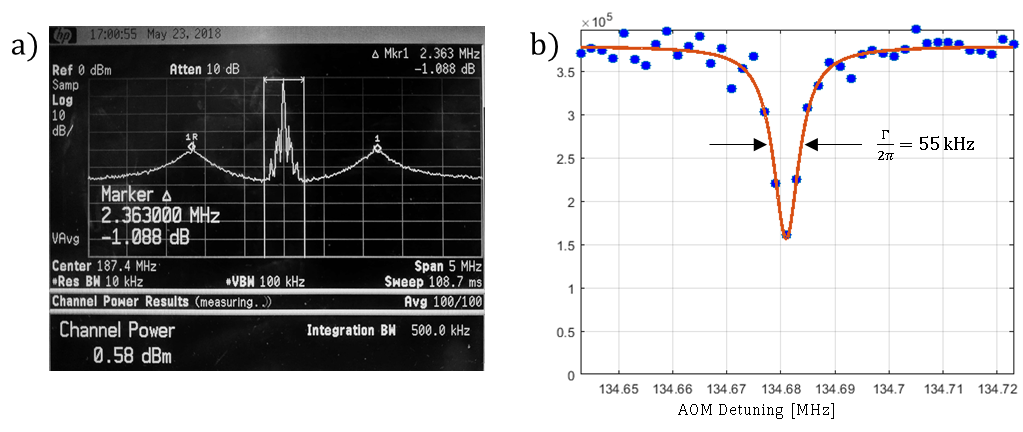
\includegraphics[width=\textwidth]{689_offsetLockCharacterization.png}}
		\caption{Characterization of the OPLL performance}{a) RF spectrum of the optical beatnote when the OPLL is engaged. Resonant peaking can be seen in the 500\,kHz band around the center frequency. b) Atom loss spectrum which shows that the resonant features are at discrete frequencies. Differences between the AOM detuning shown and the center frequency of the OPLL are due to various AOM shifts between components.}
		 \label{fig:offsetDetails}
	\end{figure}

Finally, we note that this system has also been used to perform Bragg spectroscopy as reported in the PhD thesis of Brian DeSalvo.
Detailed drawings of the optical setup used for shallow angle Bragg scattering can be found in App. \hl{something}.


\subsubsection{Spin-manipulation laser with dynamic polarization control}
Fermionic strontium 87 has become of major interest for experiments studying quantum magnetism in a highly degenerate SU(N) system. \hl{rephrease}.
Key to these studies is the creation and manipulation of arbitrary spin mixtures.
We have recently implemented a spin manipulation laser probe (spin-man) acting on the $F=9/2\,\rightarrow\,F=11/2$ hyperfine transition of the intercombination transition for the purpose of creating well defined spin mixtures.
Preliminary investigations using this system are reported in Ch. \ref{ch:chap6}.

Fig.\hl{something} highlights a simplified optical schematic of the spin-man system which is derived from slave 1 and is related to the stir MOT system outlined above in Sec. \hl{something}.
The original construction of the output optics is outlined in Ch. 5 of Josh Hill's masters work \cite{Hill2017} and is part of the layered optical systems added to the top of the optical chamber in 2017.

A major component of this layered system is the liquid crystal retarder (model: MeadowLark Optics LV-300 LCR) which allows us to dynamically control the polarization incident on the atoms.
Additionally, a configurable high precision RF system for dynamically changing the spin-man laser frequency has allowed us to demonstrate optical pumping in a magnetic field using $\sigma+$ light where we can individual address each sub-level transition independently.
Once we have spin polarized the gas, the LCR can flip the light polarization and probe the polarized ground state along the $^1S_0\,(F=9/2,m_F=9/2)\,\rightarrow\,^3P_1\,(F=9/2,m_F=7/2)$ using $\sigma-$.
Details of these experiments and further characterization of this system are presented in Ch. \ref{ch:chap6}. 

The RF tunability for optical pumping is based on the "table mode" feature of the Novatech 409B digital synthesizers which can be externally triggered to progress through a table of configured frequencies.
These synthesizers are discussed in greater detail in \hl{somewhere}.

\section{Apparatus interface} \label{sec:electronics}
\setcounter{footnote}{0}
The Neutral apparatus interfaces to our digital infrastructure via a plenitude of specialized hardware implementations and custom written software.
Over the last seven years nearly all of this digital infrastructure has been refactored, upgraded, or replaced.
Therefore, the following sections will briefly outline these new constructs, providing references to code repositories when possible.
However, detailed discussions on the usage of this infrastructure will be relegated to their respective appendices.

\subsection{Software} \label{ssec:soft_sys}
The primary control software is a custom built Labview application based on a synchronous state machine\footnote{Currently this project can be found at \texttt{https://github.com/KillianRice/neuKlein}}\hl{ref}.
The Neutral implementation of this software is called neuKLEIN (Neutral Killian Lab Experimental Interface) and is based on a major overhaul, by Joe Whalen, of the original control software.
A detailed overview of the capabilities, limitations, and instructions for use of neuKLEIN is available in App. \ref{app:neuKLEIN}.

In short, an experimental sequence begins with serially programming each voltage output device.
The pulseblasters are programmed last and are triggered via the global experimental trigger discussed in \ref{sec:expTrig} below.
Once all devices are ready the pulseblasters become the global clock and the neuKLEIN software begins polling the PixelFly camera waiting for a new image.
Once an image is received various experimental parameters are recorded into text files and saved to disk.
This process continues within the primary WHILE loop of the state machine and steps through the predetermined experimental settings array.
Primary exit conditions for the loop are encountering an error, conclusion of the settings array, or manual abortion.

Once the files are written to disk, we perform image analysis using a custom Matlab$^{TM}$ routine imaginatively named Neutral imagefit routine\footnote{Currently this project can be found at \texttt{https://github.com/KillianRice/neutral\_imagefit\_routine}}.
An in-depth discussion on the usage, extensibility, limitations, and feature improvements is available in App.\,\ref{app:imagefitManual}.

\subsection{Hardware control and measurement systems} \label{ssec:comp_sys}
The hardware control system is composed of several primary components including the experimental clock, voltage output devices, and measurement instruments.
We use a series of National Instruments$^{TM}$ data acquisition cards (NI-DAQs) and a reconfigurable FPGA for generating output voltages.
The experimental clock is based on a pair of SpinCore PulseBlaster TTL generators and a Cooke PixelFly camera is used for collecting absorption images.
We also have access to a PicoScope 5000 digital oscilloscope for high resolution signal monitoring and recording. Typically this is used for recording experiment specific photodiode signals for later analysis.

\begin{table}[]
\centerline{
\begin{tabular}{@{}|c|cc|c|cc|@{}}
\toprule
\multirow{2}{*}{Model} & \multicolumn{2}{c|}{Resolution} & \multirow{2}{*}{\begin{tabular}[c]{@{}c@{}}FIFO\\ buffer Size\end{tabular}} & \multicolumn{2}{c|}{Max sample rate} \\ \cmidrule(lr){2-3} \cmidrule(l){5-6} 
 & Bit depth & Voltage {[}mV{]} &  & Channels used & Rate {[}kS/s{]} \\ \midrule
\multirow{4}{*}{6713} & \multirow{4}{*}{12} & \multirow{4}{*}{5} & \multirow{4}{*}{16,384} & 1 - 5 & 1,000 \\
 &  &  &  & 6 & 952 \\
 &  &  &  & 7 & 833 \\
 &  &  &  & 8 & 740 \\ \midrule
\multirow{2}{*}{6221} & \multirow{2}{*}{16} & \multirow{2}{*}{0.03} & \multirow{2}{*}{8,191} & 1 & 833 \\
 &  &  &  & 2 & 740 \\ \midrule
\multirow{4}{*}{6229} & \multirow{4}{*}{16} & \multirow{4}{*}{0.03} & \multirow{4}{*}{8,191} & 1 & 833 \\
 &  &  &  & 2 & 740 \\
 &  &  &  & 3 & 666 \\
 &  &  &  & 4 & 625 \\ \midrule
\multirow{4}{*}{6733} & \multirow{4}{*}{16} & \multirow{4}{*}{0.03} & \multirow{4}{*}{16,384} & 1 - 5 & 1,000 \\
 &  &  &  & 6 & 952 \\
 &  &  &  & 7 & 869 \\
 &  &  &  & 8 & 769 \\ \bottomrule
\end{tabular}}
\caption{Arbitrary waveform generation details}{All cards specified are the PCI model and interface with the experiment control computer directly through the motherboard or via a PCI expansion bin (model: StarTech PEX2PCIE4L). Sample rates are given in kilosample per second (kS/s) and is the same across all enabled channels. The FIFO buffer stores the individual waveform points and is also shared amongst all enabled channels. Full voltage output range is $\pm$10\,V.}
\label{tab:niDaqs}
\end{table}
Table \ref{tab:niDaqs} gives the models of the NI-DAQ cards and additional details such as the resolution, the shared FIFO (first-in, first out) buffer sizes, and the maximum sample rates as a function of the number of channels in use.
Though these cards are known as acquisition cards, we instead rely heavily on the arbitrary waveform generation capabilities for dynamically generating analog output voltages.
Furthermore, we do not stream data to cards during the experimental sequence but use only the on-board FIFO buffer for storing the arbitrary waveform.

It is important to remember that the finite buffer size and maximum sample rate define two extremes for time based waveform generation due to the discretization of the waveform.
For short times, the maximum sample rate sets the minimum possible time step between two points on the voltage output.
At long times, a fixed number of points between the start and end points may lead to unacceptably large voltage steps between two points on the voltage output.
Balancing these two tradeoffs is essential and is the primary driver for the plethora of various cards so that we may dedicate their finite resources to specific tasks.

While arbitrary waveform generation is useful for dynamically varying voltages during an experimental sequence, there are a number of applications where a static voltage is needed or smoothly varying between two or more voltages is not required.
Until recently, the NI-6713 was our only sources of experimentally controlled static voltages (in contrast to a static voltage from a supply) and switching between driving voltages was done via a bank of standalone fast analog IC switches (primarily the ADG419).
Fast switching of the set point voltage has traditionally been how we control a number of systems through their feedback circuitry.
For example, the 922\,nm frequency is jumped from the optimal trapping frequency to the optimal imaging frequency at the end of the experimental sequence via the sat. abs. solenoid current.
The change in magnetic field shifts the resonance frequency of the loss feature and the 922\,nm frequency lock responds by varying the master laser frequency to restore the resonance condition.
Therefore, while imperative to retain this functionality, the NI-6713\,$+$\,switch bank limited in the number of controlled static voltages to eight and the simple standalone switches were insufficient for applying application logic for dynamically choosing driving voltages\footnote{An example of this application logic might be any set point which could be controlled via boolean logic conditioning.}.

These shortcomings led us to develop a real-time based NI-FPGA for the development of custom reconfigurable logic and static voltage output.
This system is based on a NI cRIO-9063 with integrated Artix-7 FPGA, a NI-9403 32ch TTL input/output (I/O) module, and a NI-9264 16ch analog output module.
The cRIO device manages the control layer of the system, hosting the embedded operating system and allows us to easily develop, compile, and deploy our custom control logic to the FPGA via Labview.
The FPGA (field programmable gate array) executes the user-defined logic on a user-defined loop-time (minimum 50\,$\mu$s.) with the 32 TTL I/O channels and 16 analog output available for reading and writing each cycle.
We typically do not use the output functionality of the TTL channels and instead opt for 32 input channels which can be dynamically assigned to control the 16 analog outputs.
These analog outputs may be conditioned as static, simple switched, cascading switched, or simple boolean controlled outputs all configurable via software.
Additional features include logic inputs which can be shared to multiple outputs and simple waveform generation such as linear ramps.
Detailed schematics of the input/output conditioning circuits as well as limitations, capabilities, and usage instructions are available in App. \hl{somethign}.

\subsection{Ancillary laboratory systems} \label{ssec:misc_sys}
\subsubsection{MOT coils}
The Neutral MOT coils are a complementary pair of custom made high aspect ratio solenoids which, in an anti-helmholtz configuration, can generate magnetic field gradients on the order of 150\,G/cm.
Fig.\,\ref{fig:motCoilField} shows the on-axis magnetic field.
In the center of the chamber, along the Z axis, the field gradient varies with current as 19.1\,(G/cm)/A.
	\begin{figure}
		\centerline{
		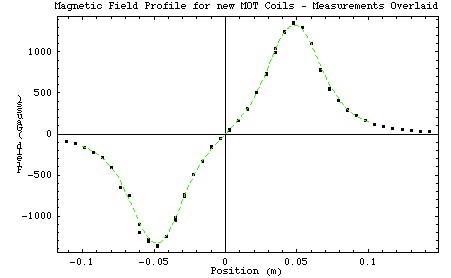
\includegraphics[width=0.75\textwidth]{misc_MOT_B_Field Profile.jpg}}
		\caption{MOT coil on-axis magnetic field}{The expected and measured B-field along the Z-axis. The measured field gradient calibration is 19.1\,(G/cm)/A}
		\label{fig:motCoilField}
	\end{figure}

\subparagraph{Historical:}
\setcounter{footnote}{0}
MOT coils were wrapped by Natali and Pascal in June of 2004.
They are wrapped using \hl{something} hollow core wire which is water cooled.
The current source in use is a \hl{something} which uses a high power FET switch to drop current across the coils.
A custom-built high-precision low resistance current sensing configuration monitors this current to actively feedback and maintain constant current through the coils \footnote{Further information and detailed notes on the wrapping can be found in \texttt{KillianDrobo:\textbackslash\textbackslash Neutral\textbackslash Laboratory Systems\textbackslash MOT Coils}}.

%\subparagraph{Potential improvement:}
%Currently the Neutral apparatus uses the same coils and supply for both the blue and red MOTs.
%However, due to the $S=1$ of the triplet system, the Zeeman shift is significantly stronger for the $^3P_1$ state. \hl{check this reasoning, the different is 1.4 MHz/G vs 2.1 MHz/G so can't be only factor}
%Consequently, we need much less current running in the MOT coils for red MOT operation.
%The blue MOT utilizes approx. 42\,Amps ($\sim$ 76\,G/cm) while the red MOT needs on the order of 100\,mAmps ($\sim 2$\,G/cm).
%These small currents for the red MOT are observed to be near the noise floor of the circuit.
%For this reason the Rydberg apparatus implemented separate red and blue MOT coils.
%We have investigated wrapping a new set of coils to follow this example but have not found a feasible to solution.
%Alternatively, we have discussed changing out the current supply dynamically between MOT operation using an H-bridge configuration as discussed in Melissa Revelle's thesis \hl{ref}.
%We have not currently pursued this option at this time.

\subsubsection{Trim coils}
Cubic trim coil cage (\hl{size?}) with the coils in a Helmholtz configuration.
These coils are used to trim out static residual B-fields and to apply dynamic and well controlled external magnetic fields.
We commonly use the coils along the Z-direction to apply bias magnetic fields during spectroscopy as shown in Fig.\,\ref{fig:trimField}a).
	\begin{figure}
		\centerline{
		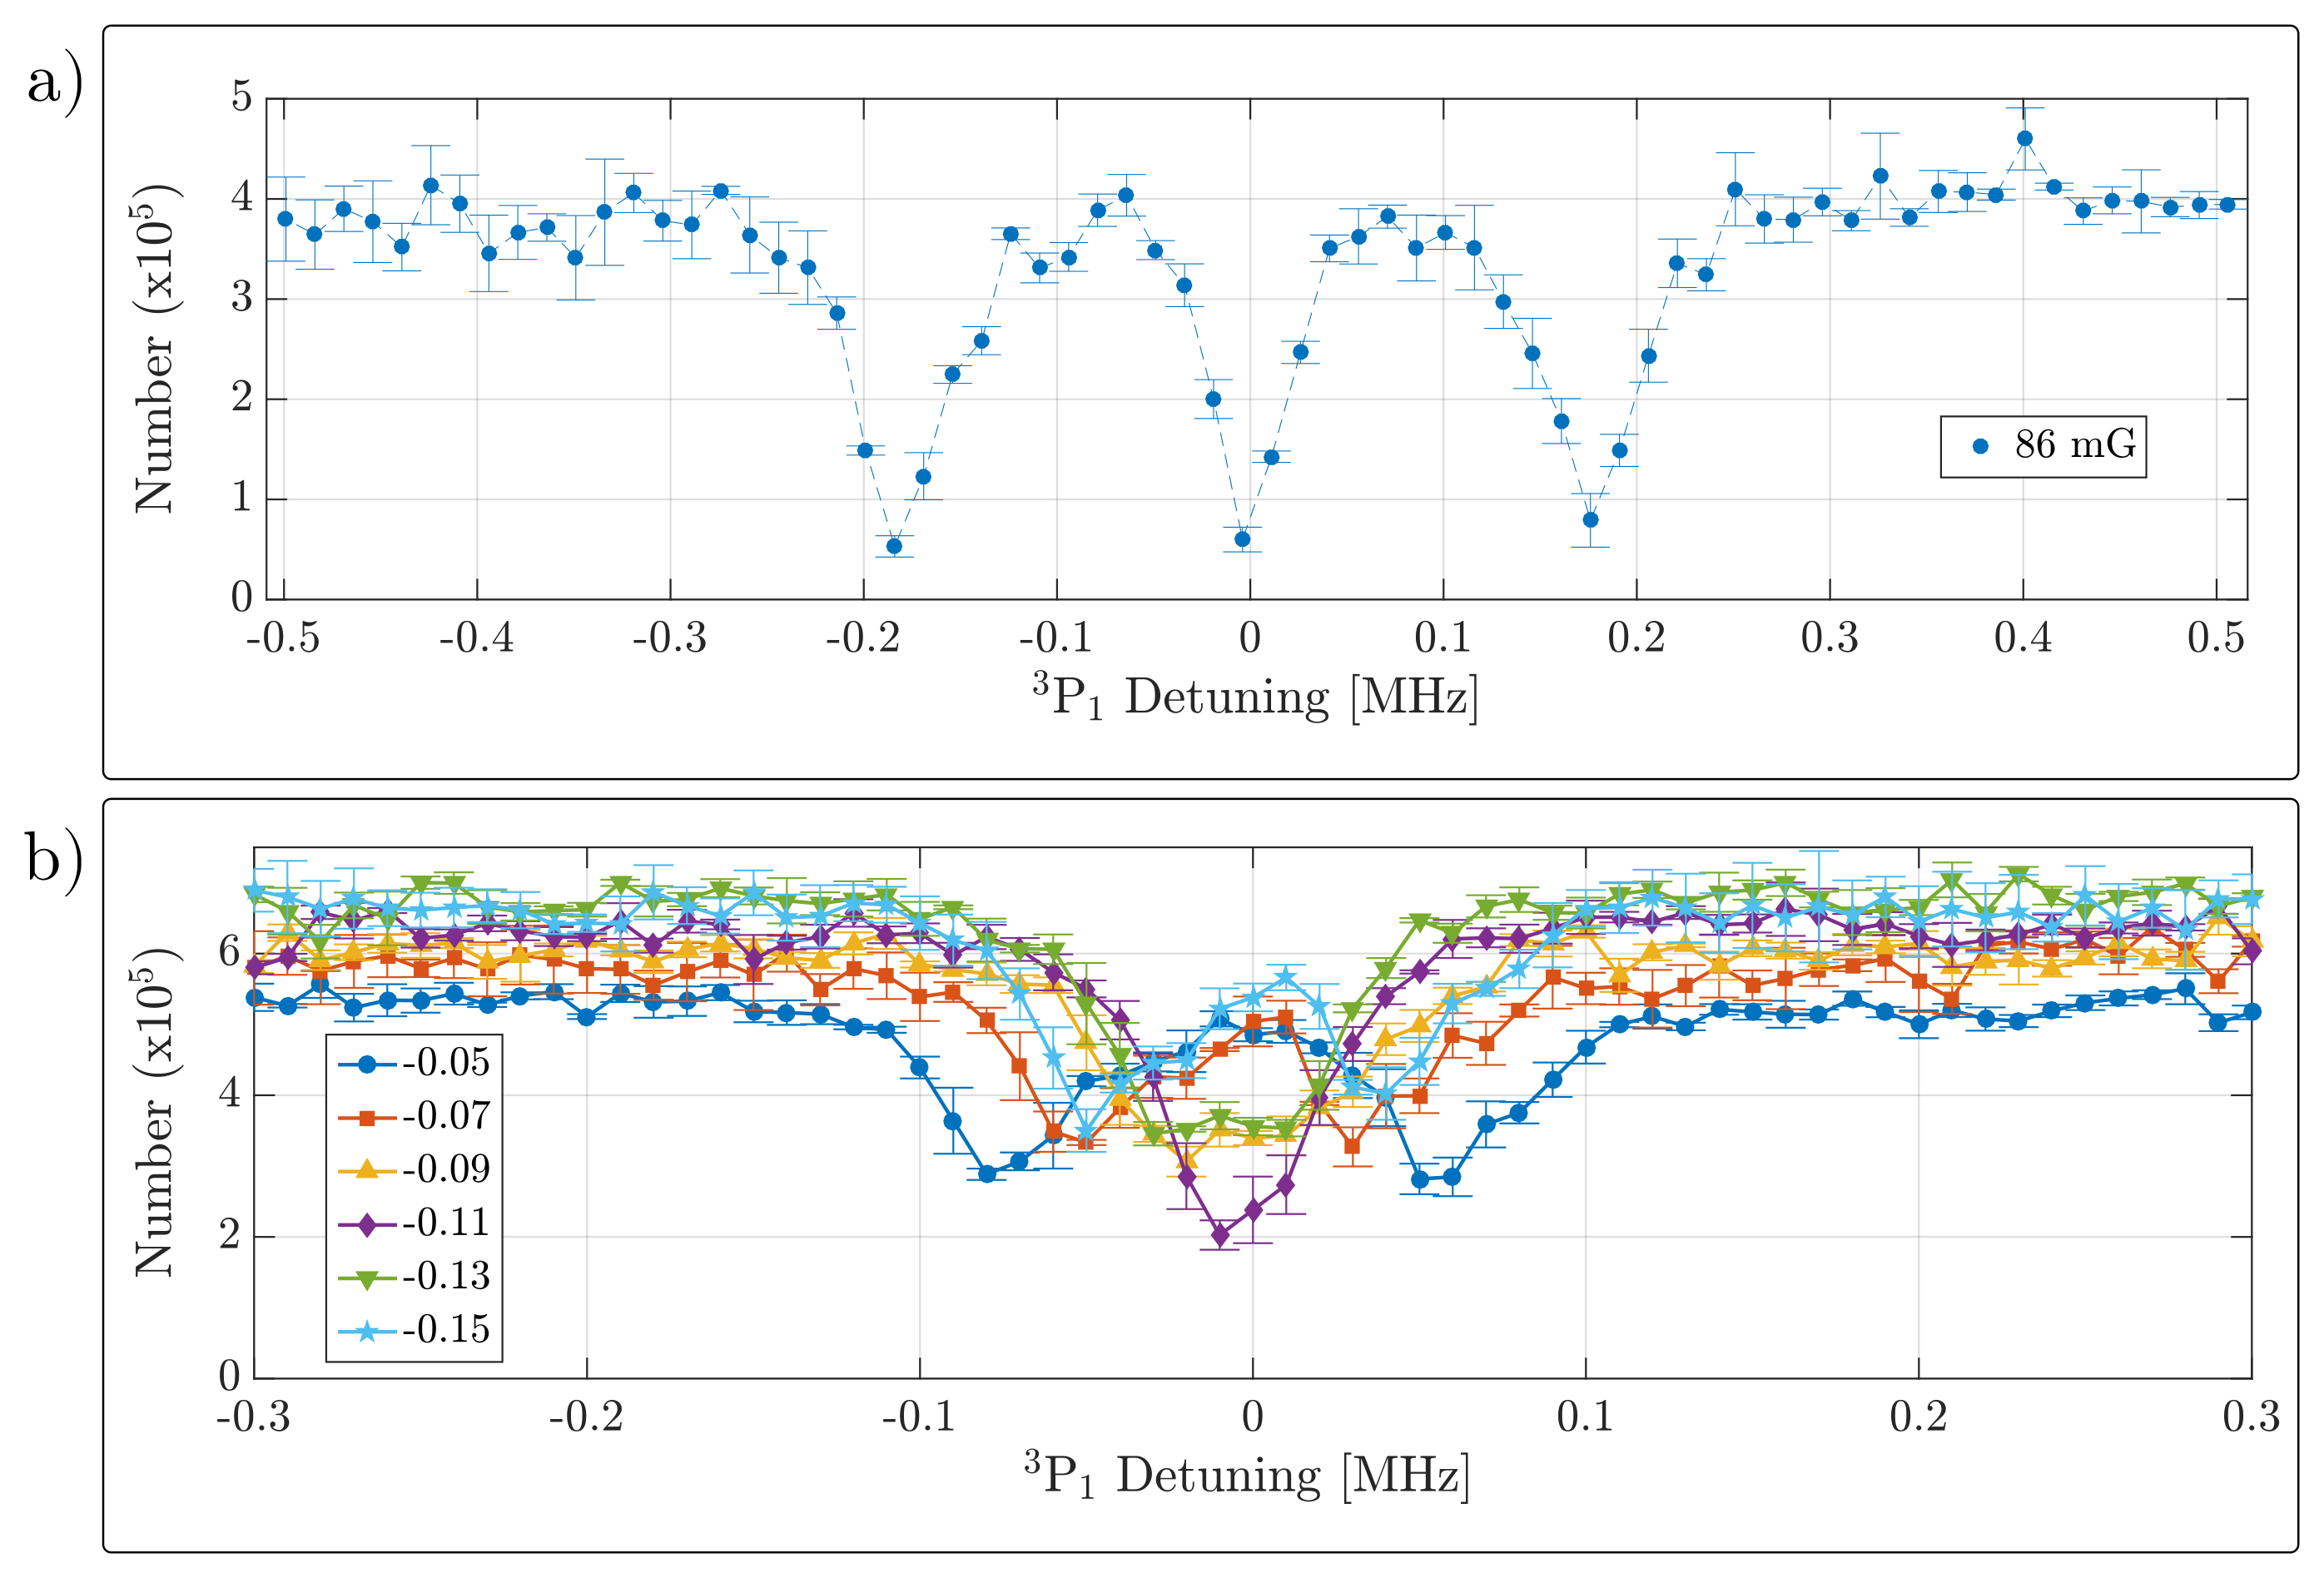
\includegraphics[width=\textwidth]{misc_trimField.png}}
		\caption{Zeroing residual magnetic fields}{Loss spectroscopy in various bias fields. a) Example of resolved Zeeman splitting of the $^3P_1$ magnetic sub-levels. b) Typical B field variation for determining the zero field position. The applied bias is increased for each subsequent scan and a clear zero crossing is observed. The legend has been left in arbitrary lab units to emphasis the B-field zero crossing which occurs around -0.11.}
		\label{fig:trimField}
	\end{figure} 
	
The fine-structure magnetic sub-levels of the $^3P_1$ state vary with B-field as 2.1\,MHz/G.
Compared to the natural linewidth of 7.5\,kHz, this splitting of the $^3P_1$ states provides a very sensitive probe for precisely zeroing the residual magnetic field.
We determine the required bias fields by performing loss spectroscopy with unpolarized light along the $^1S_0\,\rightarrow\,^3P_1$ transition using a bosonic isotope.
Next we fit the $m_j=\pm1$ spectral features to a loss line-shape (either gaussian or lorentzian) and plot the line center as a function of applied magnetic field along each dimension.
Fig.\,\ref{fig:trimField}b) shows an example of the change in Zeeman splitting of the m$_j$ levels using strontium-84.
Finally, we perform a linear fit to the line center variation and extract the intercept which nulls the residual field and the slope which calibrates our applicable field strength per ampere. 
We have found these calibrations to be [$\delta B_z = 0.985, \delta B_y = 0.982, \delta B_z = 0.987$]\,G/A\footnote{Further details available in Onenote under Research Projects $\rightarrow$ Routine Studies $\rightarrow$ B-field zeroing $\rightarrow$ Zeroing summary}.

\subsubsection{Zero crossing AC line trigger} \label{sec:expTrig}
Fig.\,\ref{fig:zeroCrossTrig} shows the circuit used to start the Neutral experimental sequence.
	\begin{figure}
		\centerline{
		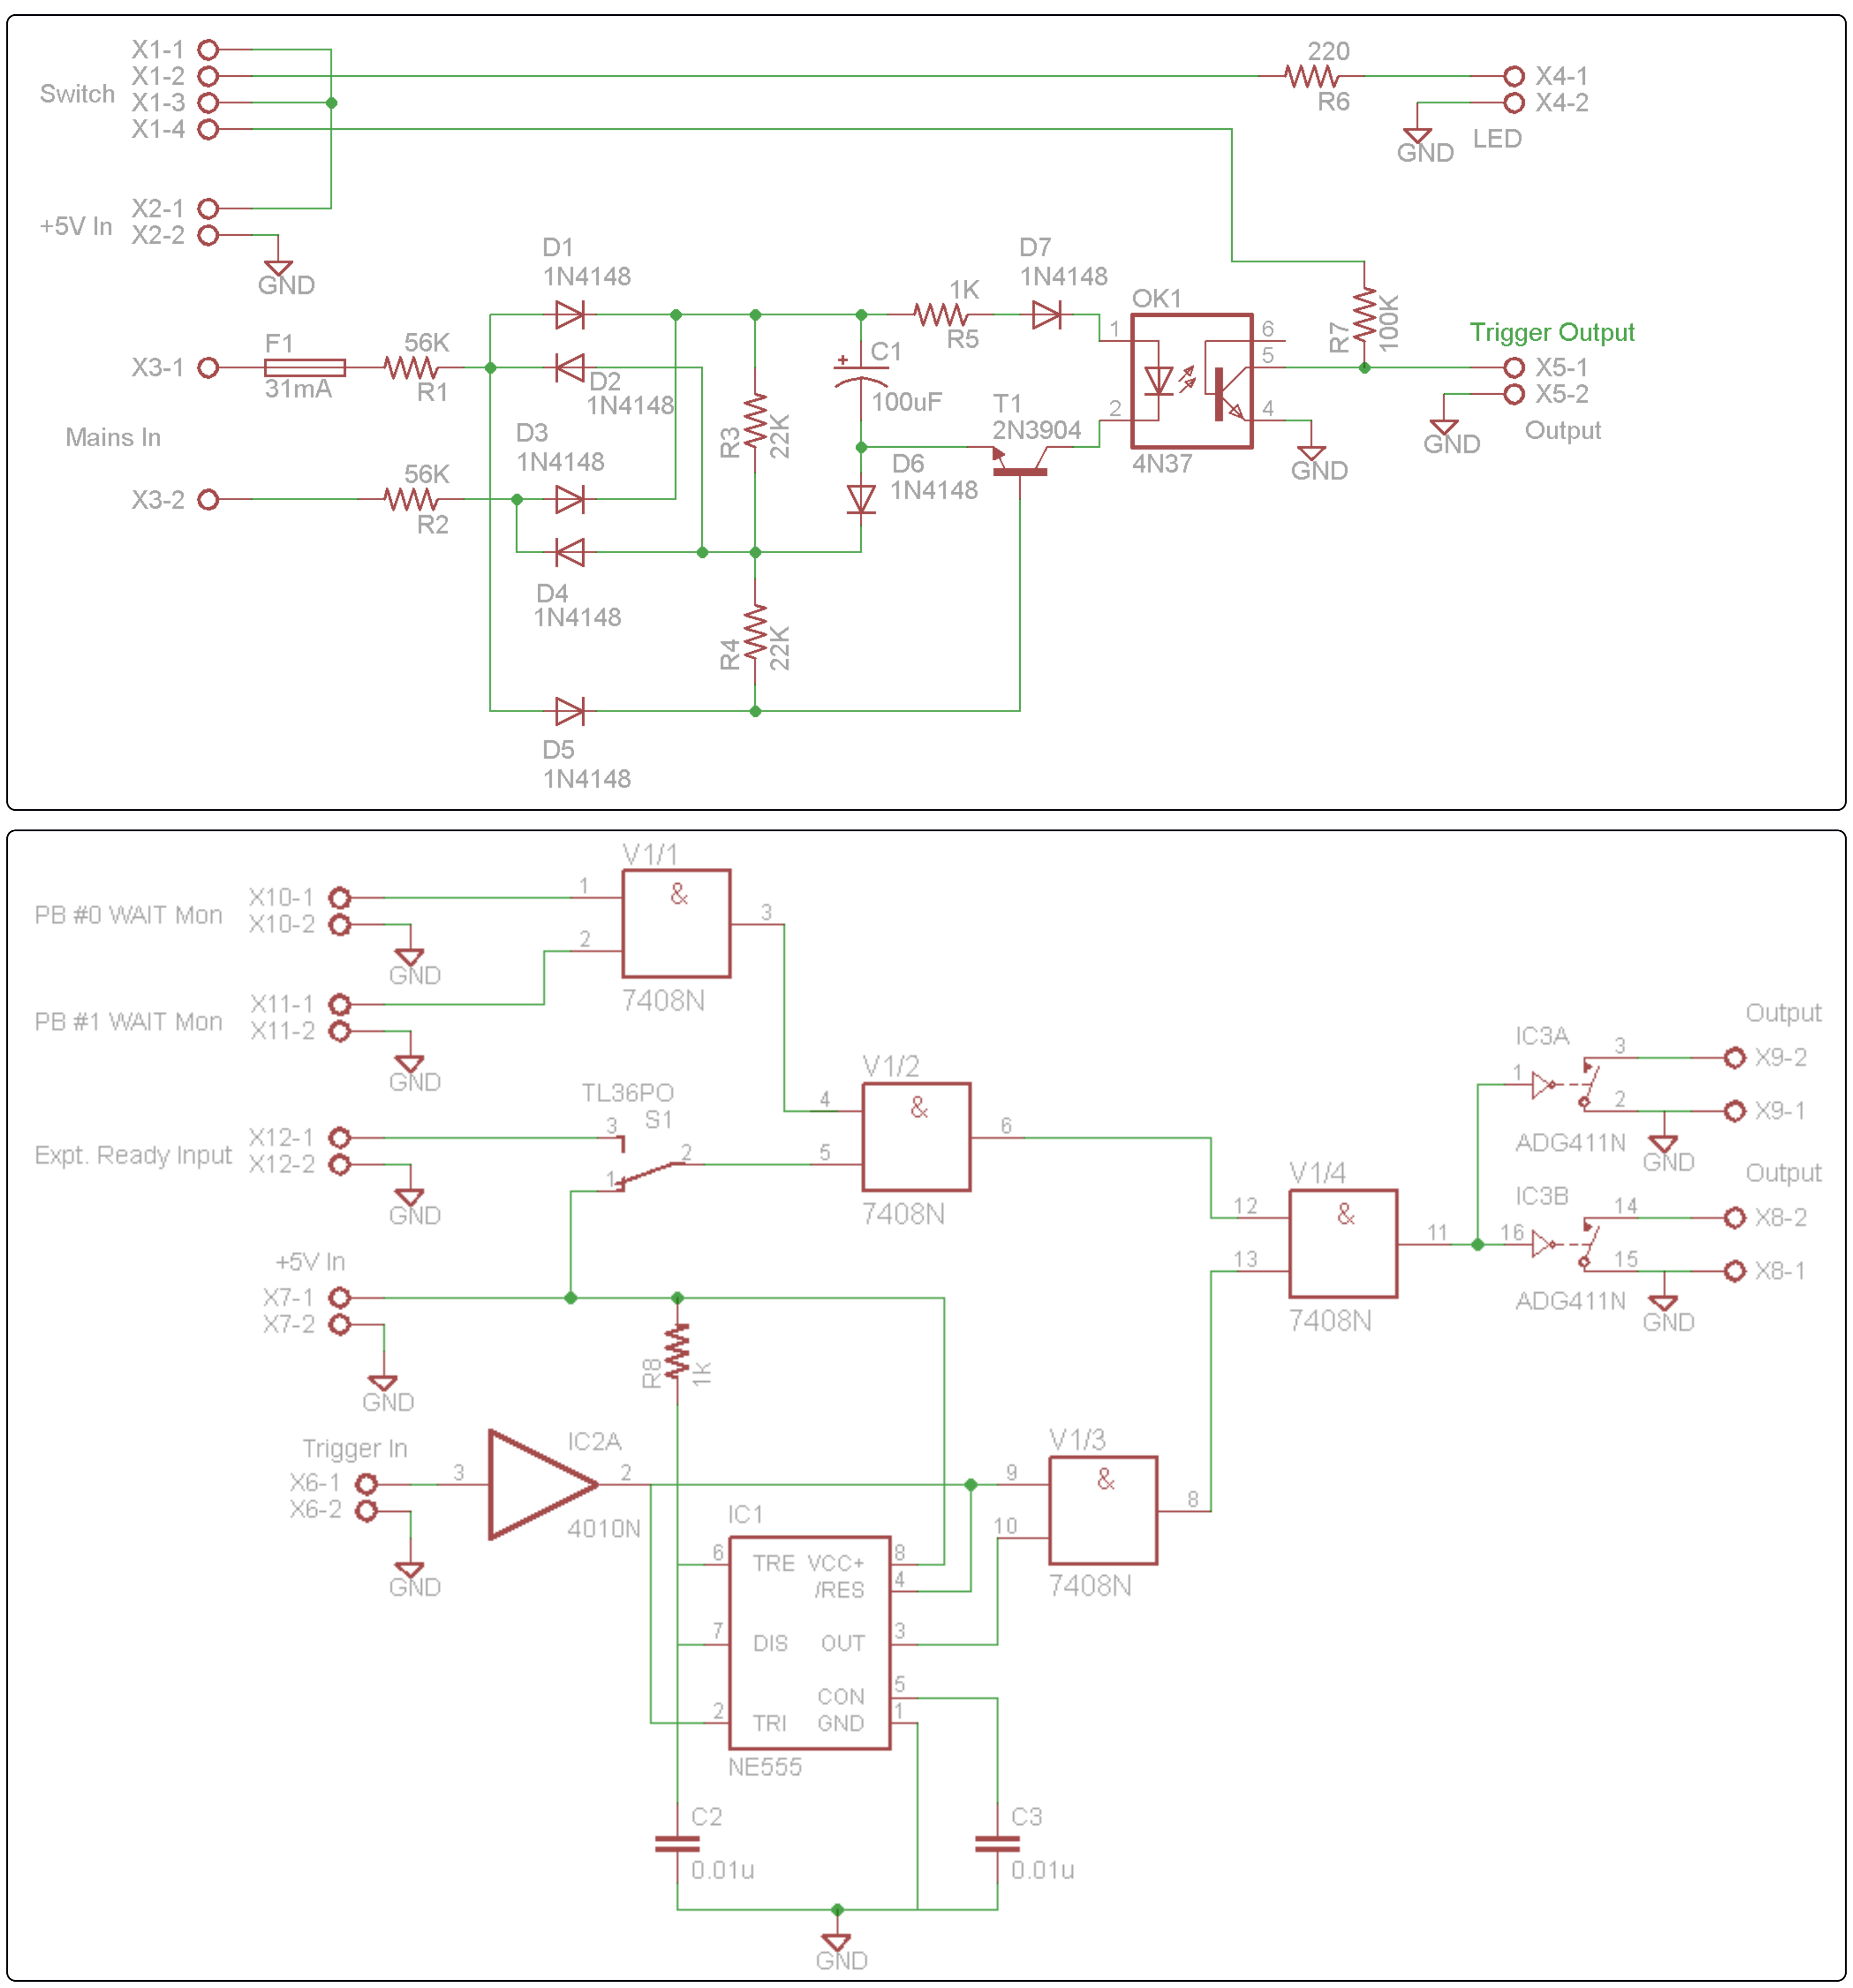
\includegraphics[width=\textwidth]{misc_acZeroCrossingSyncTrigger.png}}
		\caption{Circuit diagram of the zero crossing AC line trigger}{Top - 120\,Hz square wave pulser which generates a short pulse on the 60\,Hz zero crossing. Bottom - Synchronizer circuit between both pulseblasters, an optional expt. ready trigger (which ensures the atom shutter is open), and the AC zero-crossing trigger. Trigger input is from the top circuit and is used with the 555 timer in a one-shot configuration. This ensures only every other pulse from the AC trigger produces a HI output past the AND gate V1/3.}
		\label{fig:zeroCrossTrig}
	\end{figure} 
It is based on deriving a TTL pulse at the positive-going zero crossing of the 60\,Hz building line.
Manual triggering is essential since we do not share the same clock source between the two independent pulseblasters (PB0\,\&\,PB1).
Instead relying on their relative precision and low timing jitter to maintain experimental synchronicity when triggered from a shared source.
Fig.\,\ref{pbTimingJitter} shows a comparison of the timing uncertainty when a short 200\,ns pulse is output from both pulseblasters and the oscilloscope is triggered from the zero crossing of the AC line.
	\begin{figure}
		\centerline{
		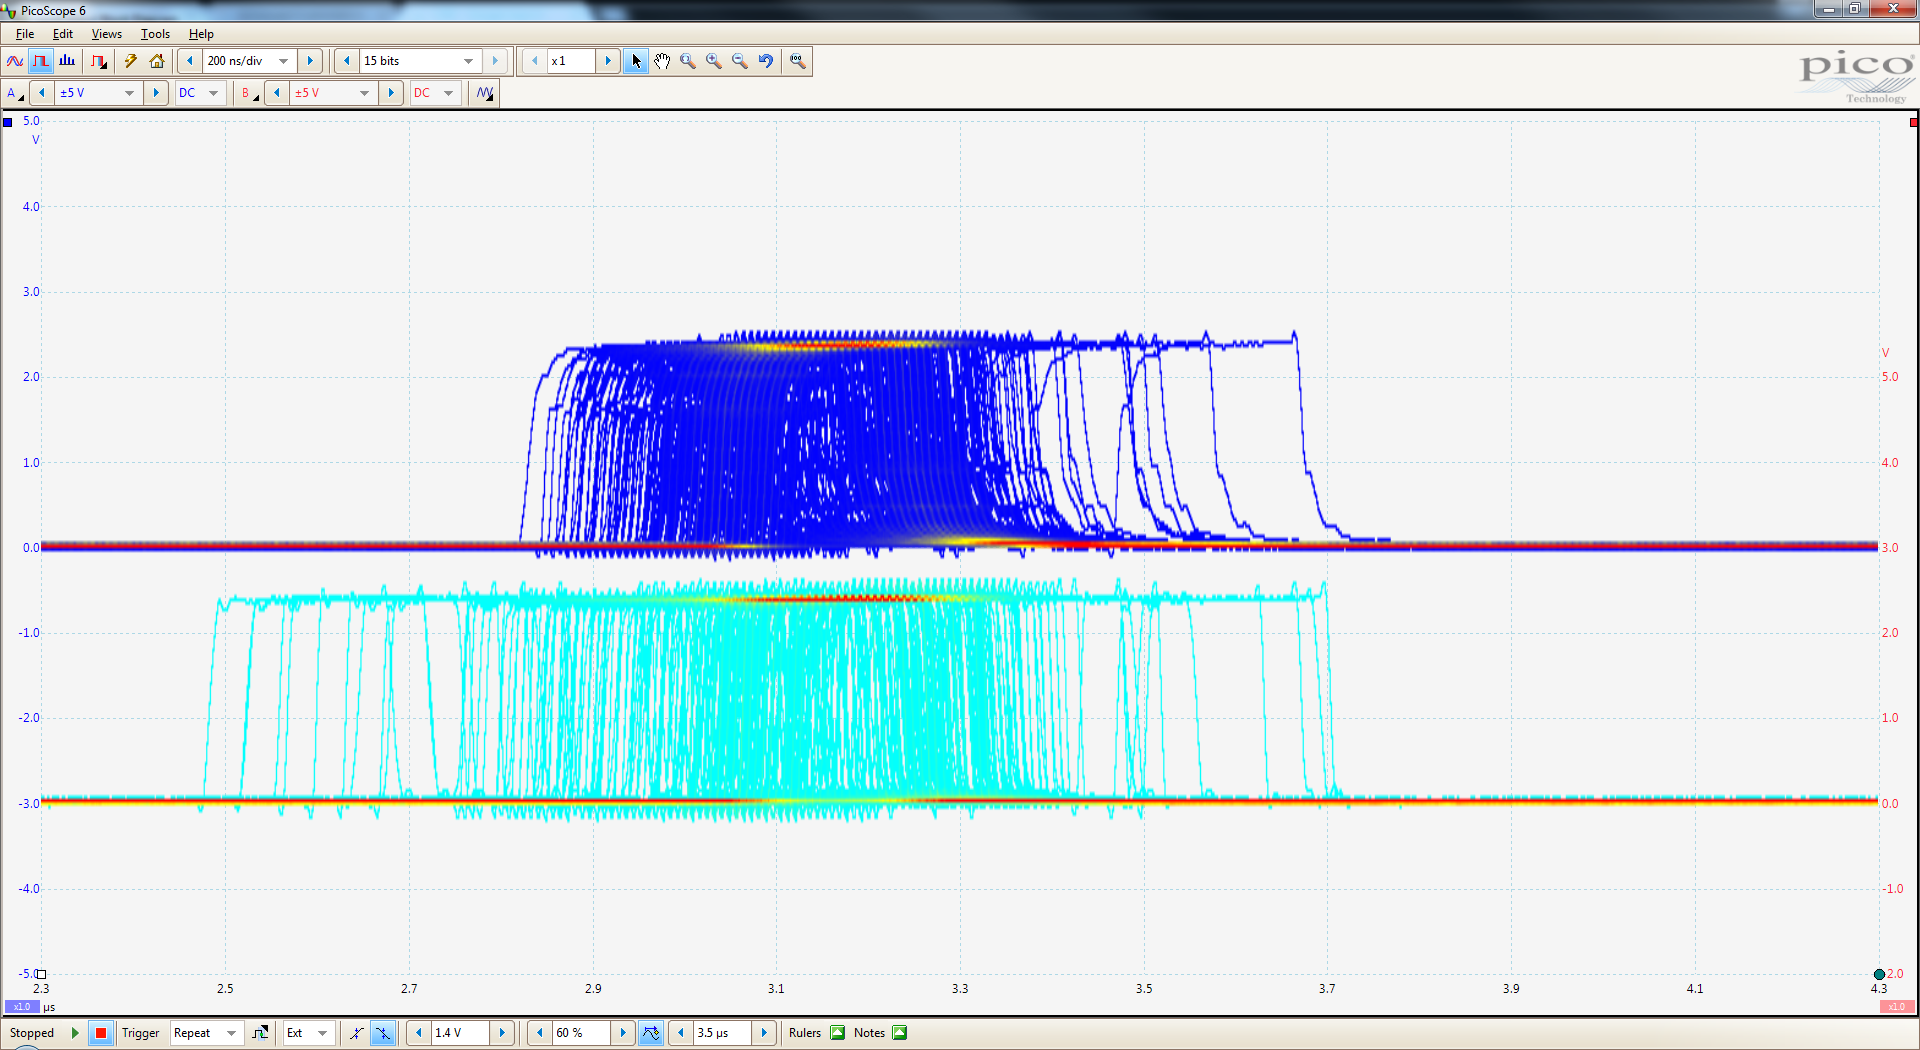
\includegraphics[width=\textwidth]{misc_PB_TriggerJitter.png}}
		\caption{Comparison of pulseblaster timing jitter}{A persistent oscilloscope trace showing repeated measurements of a 200\,ns logic pulse from each pulseblaster. The upper signal is PB0 and the lower is PB1. The scope is externally triggered by the zero crossing AC line trigger.}
		\label{fig:pbTimingJitter}
	\end{figure} 
While this measurement does not reveal the cause of the relative instability between the three sources (PB0, PB1, or AC line), we do observe a relative instability of approx. 1\,$\mu$s.
For most use cases with ultracold matter, this timing uncertainty is entirely reasonable and presents no practical limitation.
However, this behavior does preclude the usage of cross-triggers between the pulseblasters when performing experiments with the optical lattice\footnote{Cross-triggers are defined as the mixing of timing signals between the two pulseblasters.
For instance, using PB0 to trigger the turn on of lattice arm A and PB1 to trigger arm B.}.
This timing difference results in a similar consideration as the discrete timing issue discussed previously whereby, dependent on the dynamics under investigation, even small timing difference can lead to significant variation in the observed phenomena.
We mitigate this effect by taking care to trigger all related processes from the same pulseblaster where the timing jitter is reduced to 50\,ns.

We choose to trigger off the building wide 60\,Hz line in order to maintain a fixed phase relationship from shot to shot.
This is thought to act as a common-mode rejection of electrical noise which could couple into our measurements via intensity or frequency noise.
However, we have not rigorously evaluated this hypothesis and no significant change was observed when changing the global experimental trigger.

Finally, the additional logic gates ensure that the pulseblasters trigger at the same time since they are programmed serially by the neuKLEIN software.
This process is enabled by a WAIT signal that each pulseblaster outputs when in this state which is used to ensure proper initialization of the system before starting an experimental sequence.

\subsubsection{Pneumatic actuated mirror mounts}
One challenge of using a 532\,nm optical lattice is that this wavelength is between the 461\,nm and 689\,nm wavelengths used for our MOT beams and the 532\,nm must operate at high power.
For the lattice arms in the plane of the atoms (A \& B) we combine and separate the lattice light along the 1064\,nm ODT path using common harmonic beamsplitters.
However, the vertical path (arm C) presents a significant challenge as the numerical aperture along this path into the chamber is restricted by the MOT coils.
Moreover, maintaining clean polarization of the MOT beams requires us to place the MOT waveplate along the vertical axis so as to avoid mirror reflections which may rotate the polarization.
This places prohibitive constraints on the availability of passive optical components which might combine the MOT and lattice traps.
Currently, we employ industrial pneumatic valves (model: \hl{model}) with actuators (model: \hl{moel}) to move the waveplates and requisite MOT mirrors out of the path before turning on the 532\,nm light.
Fig.\,\ref{fig:pnuSys} shows the flow diagram for switches S1 and S2 for this system.
	\begin{figure}
		\centerline{
		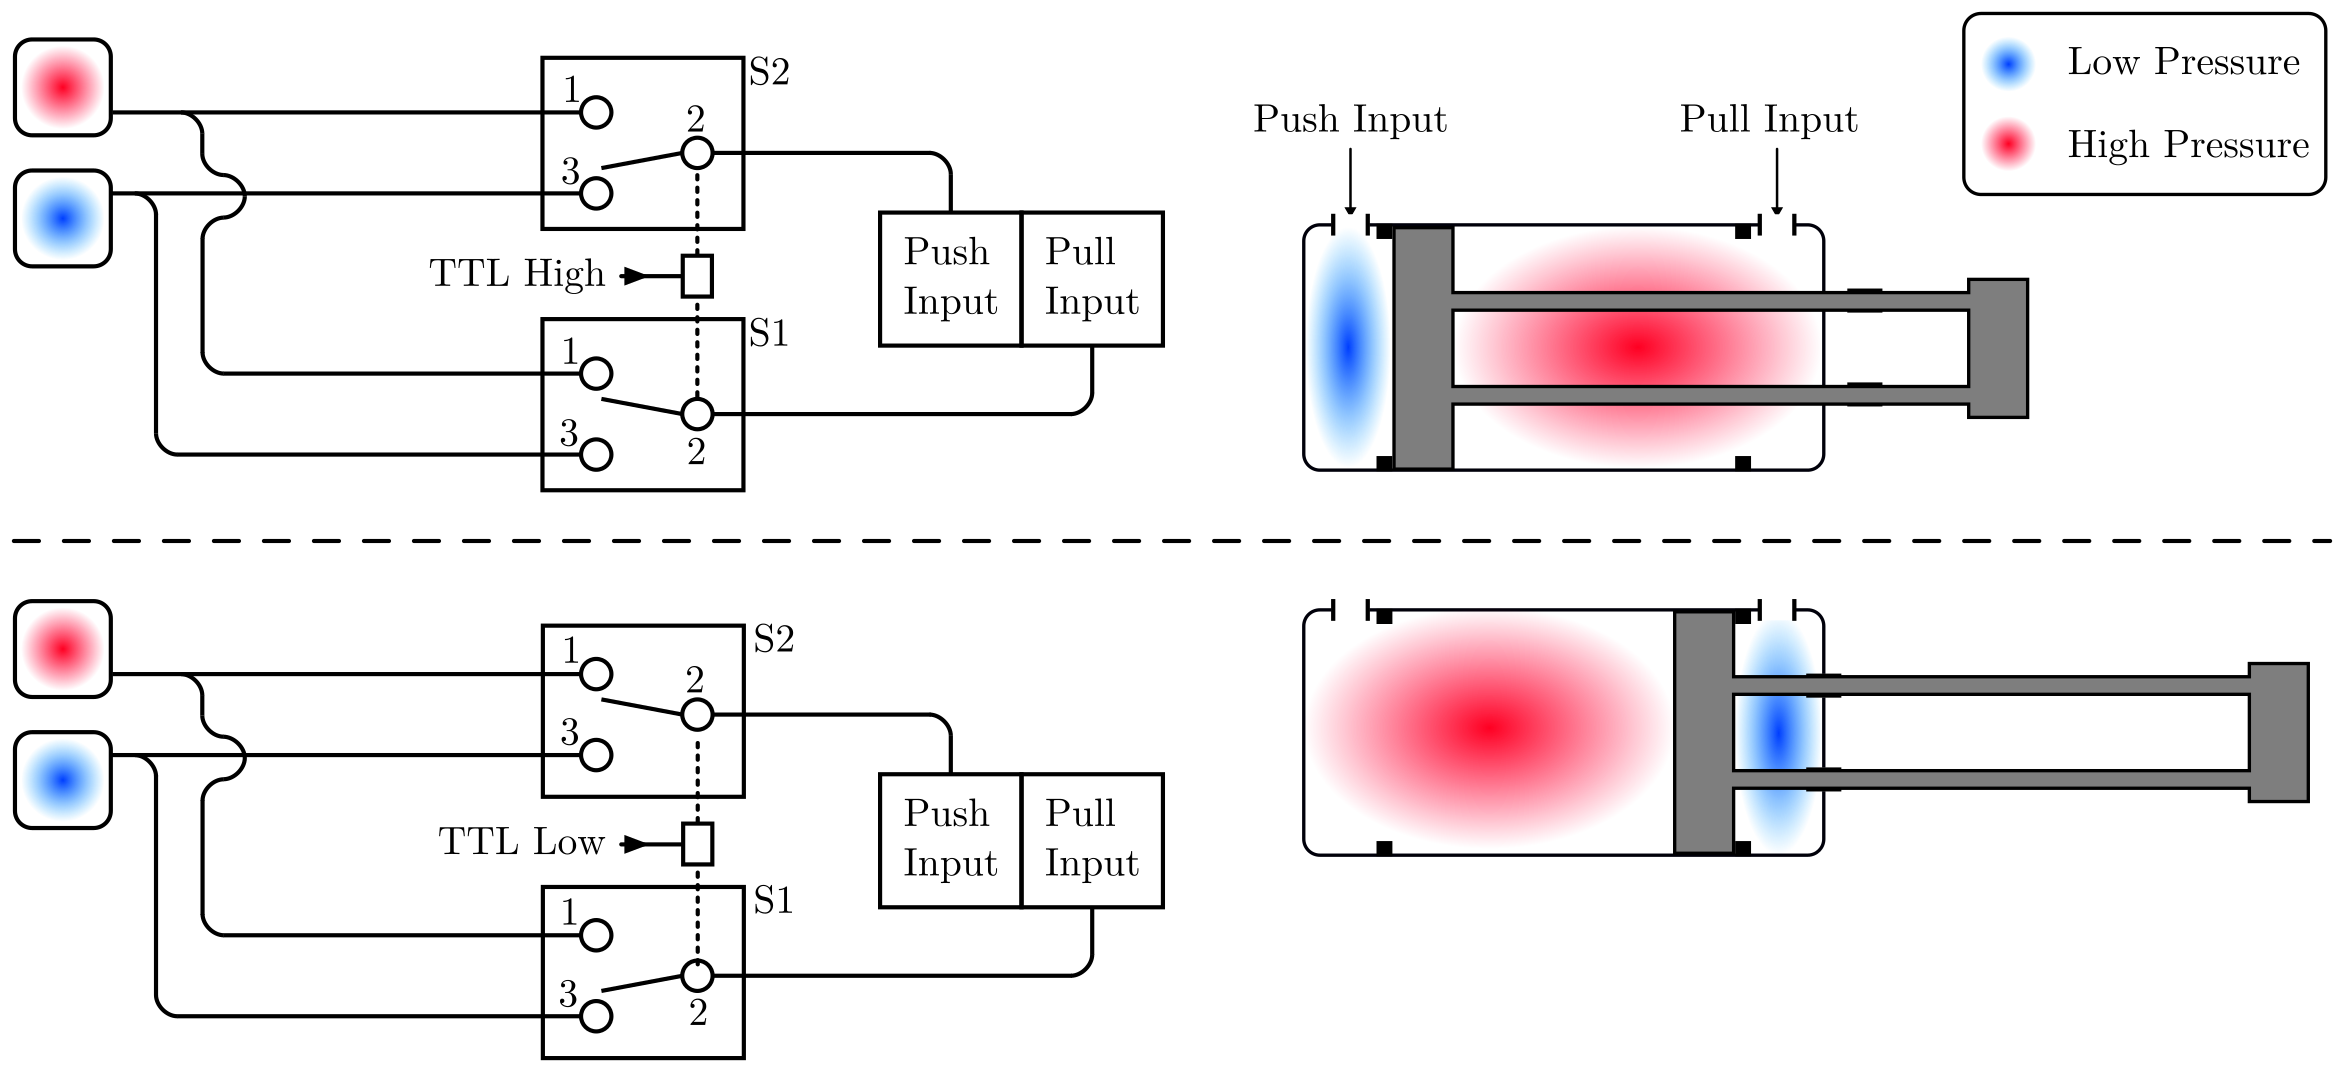
\includegraphics[width=\textwidth]{misc_pneumaticSystem.png}}
		\caption{Pneumatic actuators diagram}{Example schematic for a single actuator. Three actuators are used on the apparatus to move several components simultaneously. Not shown is the 4-way cross which splits the output from each valve (S1 and S2) to each actuator.}
		\label{fig:pnuSys}
	\end{figure}
As one might expect, this abrupt movement does impart vibrations into to the table which we dampen by slowing the movement and cushioning the stops.
In practice we find that the system is fairly robust against these small "kicks" though occasionally the air pressure must be adjusted if the lasers are behaving erratically..
We have also observed a settling of the actuators when extended as this is this default position.
Future improvements may aim to provide a rail system for guiding the movement and supporting the actuators against gravity for smoother movement.